\documentclass[12pt]{article}
\usepackage[utf8]{inputenc}
\usepackage[a4paper, total={6in, 8in}, margin=1in]{geometry}
\usepackage{titlesec}
%\usepackage[style=ieee, backend=biber]{biblatex}
\usepackage{graphicx}
\usepackage{amsmath}
\usepackage{amssymb}
\usepackage{amstext}
\usepackage{enumitem}
\usepackage{siunitx}
\usepackage{array}
\usepackage{xcolor}
\usepackage{multirow}
\usepackage{hyperref}
\usepackage{tabularx}
\usepackage{booktabs}
\usepackage{soul}
\usepackage{fancyhdr}
\usepackage{setspace}

\hypersetup{
    colorlinks=true,
    linkcolor=blue,
    filecolor=magenta,
    urlcolor=blue,
    pdftitle={aes670hw2},
    pdfpagemode=FullScreen,
    }
\urlstyle{same}

\newcolumntype{L}{>{$}l<{$}}  % Math mode table
\newcolumntype{R}{>{$}r<{$}}  % Math mode table
\newcolumntype{C}{>{$}c<{$}}  % Math mode table

\pagestyle{fancy}

\renewcommand{\sectionmark}[1]{%
\markboth{\thesection\quad #1}{}}
\fancyhead{}
\fancyhead[L]{\leftmark}
\fancyfoot{}
\fancyfoot[C]{\thepage}

\bibliographystyle{ieeetr}
%\addbibresource{main.bib}
%\bibliography{main}

\definecolor{Light}{gray}{.9}
\sethlcolor{Light}

\newcommand{\hltexttt}[1]{\texttt{\hl{#1}}}


\titleformat{\section}
  {\normalfont\fontsize{14}{15}\bfseries}{\thesection}{1em}{}

\titleformat{\subsection}
  {\normalfont\fontsize{12}{15}\bfseries}{\thesubsection}{1em}{}

\title{AES 770 Satellite Remote Sensing II

Cloud Property Retrieval}
 \author{Mitchell Dodson}
\date{September 15, 2023}

\begin{document}

\maketitle

\vspace{-2em}

\begin{figure}[h!]
    \centering
    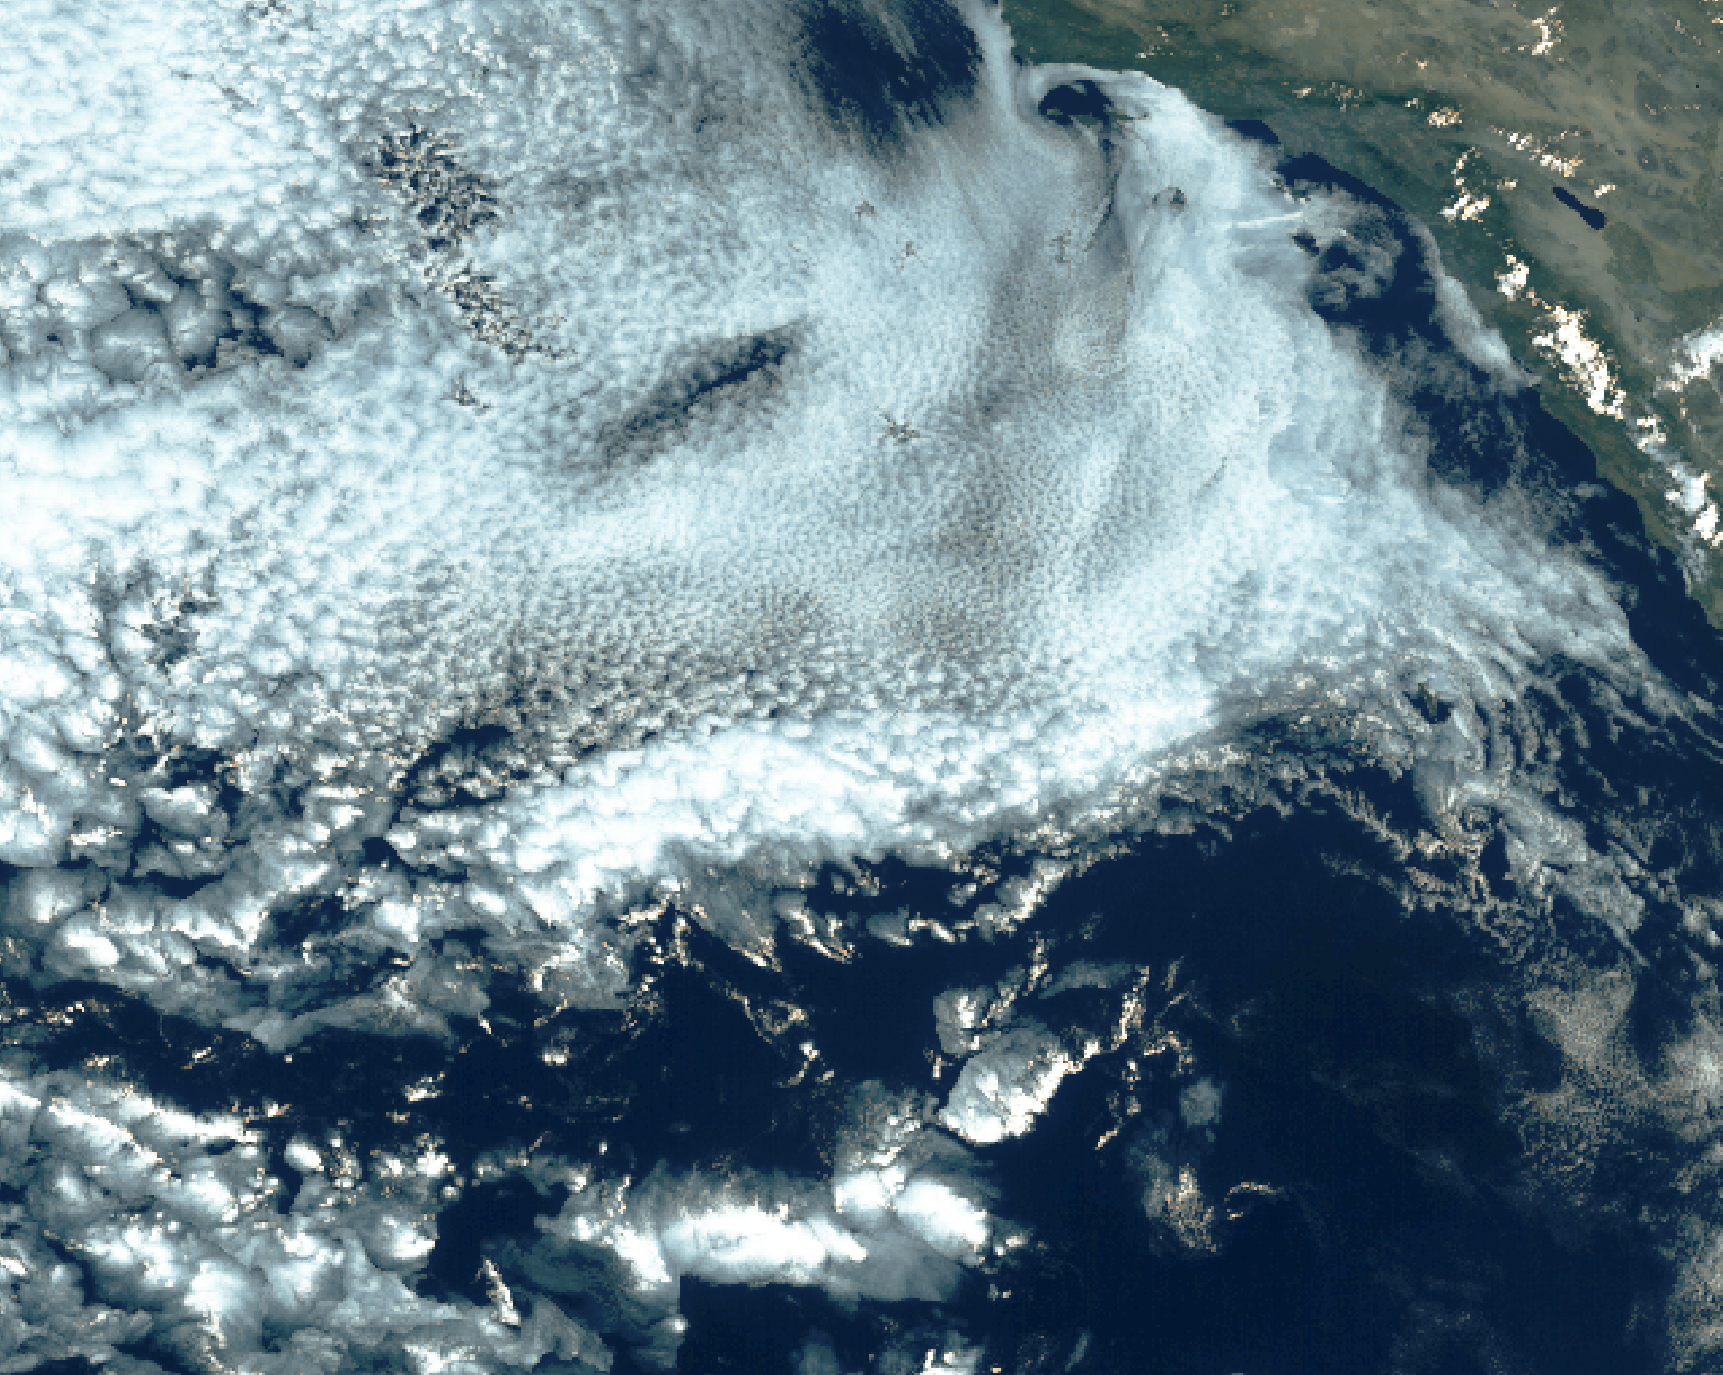
\includegraphics[width=.6\paperwidth]{figs/region-tc.png}
    \caption{Enhanced ABI Truecolor image of my chosen region, captured by GOES-18 on October 27, 2022 at 1927z. The domain is centered around $29^\circ$ N, $123^\circ$ W, off the coast of Baja, California, and covers a total surface area of about $1,327,600\,\si{km}$. Features include stratocumulus water clouds with a variety of optical properties, as well as dense low-lying fog over California.}
    \label{title_image}
\end{figure}

\section{Abstract}

This document outlines my implementation of a cloud property retrieval algorithm for ABI L1b radiances in channels 2 ($0.64\mu m$) and 6 ($2.24\mu m$). The retrieval process leverages the differences in the reflectance function of clouds in the conservative-scattering and absorbing channels in order to estimate the top-of-cloud optical depths (COD) and effective radii (CRE) of pixels identified as water clouds by maximum-likelihood classification. COD and CRE estimates are are important inputs for other retrieval algorithms as well as climate models since the two parameters can almost fully characterize the radiative properties of clouds \cite{slingo_gcm_1989}.

%\clearpage
%\section{Code comment}\label{code_comment}

\clearpage

\section{Theoretical Basis}

\begin{figure}[h!]
    \begin{equation}\label{toa_ref}
        \begin{split}
            R_{TOA} &= R_c(\theta_0, \theta, \Delta \phi, \tau_c, r_e) + R_e(\tau_c, r_e) + \\
            &+ R_{ray}(\theta, \theta_0, H, \tau_r, \tau_c, r_e) + R_{tran}(\theta, \theta_0, A_s, \tau_r, r_e) %\frac{A_s t_c(\tau_c, r_e, \theta) t_c(\tau_c, r_e, \theta_0)}{A_sR_c(\tau_c, r_e)}
        \end{split}
    \end{equation}
    \caption{Generalized expression for top-of-atmosphere reflectance. $R_c$ is the actual cloud layer's reflectance function, $R_e$ is the effective reflectivity contributed by thermal emissions, $R_{ray}$ represents the increment of reflectance from above-cloud rayleigh scattering, and $R_{tran}$ specifies the radiation transmitted through the cloud, reflected by the surface, and transmitted through the cloud once again.}
\end{figure}

\subsection{Spectral Reflectivity of Clouds}

Cloud property retrievals make inferences by comparing simultaneous measurements of backscattered cloud reflectance in a visible waveband near $0.64\mu m$ and a water-absorbing near-infrared band such as $2.24\mu m$ or $3.9\mu m$. Since the single-scattering albedo of water in the visible range is close to 1, it's reasonable to assume that a cloud layer's reflectivity in such a channel is dominantly determined by the layer's optical thickness $\tau_c$ and the viewing geometry at the pixel location. In contrast, the above near-infrared channels strongly attenuate solar irradiance by absorption, the magnitude of which correlates with the volume extinction coefficient of water droplets $\sigma_e = \pi r^2 Q_e$. Due to the nonlinear relationship between absorption and the geometric size of cloud particles, the observed reflectances are more directly related to the \textit{effective radius} $r_e$ as identified by (Hansen and Travis, 1974) \cite{hansen_light_1974}. This quantity is defined as the ratio between the third and second moments of the cloud particle size distribution, and can be thought of as the physical radius particles in a completely uniform cloud layer would need to have in order to match the observed polydisperse cloud's reflectance.

Aside from the influence of physical cloud properties $\tau_c$ and $r_e$, the cloud reflectance function $R_c$ is also highly dependent on the viewing geometry of the Sun/surface/satellite system, which in this case consists of the solar zenith angle $\theta_0$, viewing zenith angle $\theta$, and relative azimuth angle $\Delta \phi$. These angles are important because they determine the path length of radiation through the cloud, the flux density at the cloud surface, and the reflected radiance in the particular direction of the sensor (which depends on the scattering phase function of cloud particles). Theoretical representations of the cloud layer reflectance function $R_c$ based on thick-layer asymptotic expressions are outlined by (King, 1983) and (King, 1987) for conservative-scattering and absorbing wavebands respectively \cite{king_determination_1987}\cite{king_number_1983}, however for this application all the above considerations are handled by Mie code evaluated by the SBDART radiative transfer model.

\subsection{Surface, Rayleigh, and Emission Correction}

The top-of-atmosphere radiances observed by ABI are also affected by radiation transmitted back through the cloud after being reflected by the surface, additional radiation scattered into the path by above-cloud rayleigh effects, and by additional radiance from thermal emission. The first situation, represented by $R_{tran}$ in Equation \ref{toa_ref}, is a function of cloud transmission $t_c$ and surface albedo $A_s$, typically expressed as $\left(A_s t_c(\tau_c, r_e, \theta) t_c(\tau_c, r_e, \theta_0)\right)\left(A_sR_c(\tau_c, r_e)\right)^{-1}$.

The second case includes photons that are only sent into the sensor aperture because of a rayleigh single-scatter interaction with the atmosphere above the cloud. These interactions are enumerated by (Wang and King, 1997) and include (1) atmosphere$\to$sensor, (2) atmosphere$\to$cloud$\to$sensor, and (3) cloud$\to$atmosphere$\to$sensor \cite{wang_correction_1997}. The rayleigh cases are modeled by $R_{ray}$ in Equation \ref{toa_ref}, and are only relevant for the visible channels since rayleigh scattering is negligible for the longer wavelengths in the near-infrared range.

Finally, $R_e$ represents additional radiance from thermal emission, which is significant if the absorption channel used is near the SWIR $3.9\mu m$ range, and may even influence results in the $2.24\mu m$ channel for edge cases with very hot surface temperatures such as below-cloud fire hot spots. For my retrievals, the first 2 situations are considered by SBDART as it performs layerwise discrete ordinate calculations.

\section{Lookup Table Generation}

\begin{table}[h!]
    \centering
    \begin{tabular}{ m{.15\linewidth} | m{.15\linewidth} | m{0.6\linewidth}}
        \textbf{Parameter} & \textbf{Value} & \textbf{Justification} \\
        \hline
        PHI; NPHI & [0,180]; 12 & $12^\circ$ even increments of relative azimuth angles. \\
        \hline
        UZEN; NZEN & [0,84]; 21 & $4^\circ$ even increments of viewing zenith angles. \\
        \hline
        SZA & [0,84]; 21 & $4^\circ$ even increments of solar zenith angle. \\
        \hline
        TCLOUD & [0.1,160]; 40 & Logarithmically spaced increments of cloud optical depth. \\
        \hline
        NRE & [2,80]; 40 & Logarithmically spaced increments of cloud effective radius. \\
        \hline
        WL & $0.64\mu m$ $1.24\mu m$ $3.9\mu m$ & Generate independent lookup tables for VIS, NIR, and SWIR channels. \\
        \hline
        IDATM & 2 & Mid-latitude summer; $2.294\,\si{g.cm^{-2}}$ column water vapor to approximate subtropical oceanic profile. \\
        \hline
        ISAT & 3 & GOES West relative spectral response functions. \\
        \hline
        ISALB & 7 & Ocean surface albedo ID. \\
        \hline
        BTEMP & 292 & Mode longwave-window brightness temperature of ocean surface class ($\si{K}$). \\
        \hline
        ZCLOUD & 2 & Approximate cloud height calculated using integrated hypsometric equation given mode temperatures of ocean and dense-cloud surface classes. \\
    \end{tabular}
    \caption{Outline of the SBDART parameters used for the generation of lookup tables}
    \label{sbdart_params}
\end{table}

An ideal cloud property retrieval would entail solving Equation \ref{toa_ref} for $\tau_c$ and $r_e$ as a function of the observed reflectance and other known properties (geometry, cloud height, surface albedo, etc), however an analytic solution is far from possible. Thus, in order to establish a theoretical basis for optimal estimate inversion, we must generate a lookup table consisting of axes covering the full valid range of each variable. Using the parameters in Table \ref{sbdart_params}, I created a 5-dimensional lookup table for each of the relevant wavelengths, each of which ultimately have entries indexed by coordinates in the specified ranges like (solar\_zenith, optical\_depth, effective\_radius, viewing\_zenith, relative\_azimuth).

\clearpage

\begin{figure}[h!]
    \centering
    \begin{center}
        \makebox[\textwidth]{
            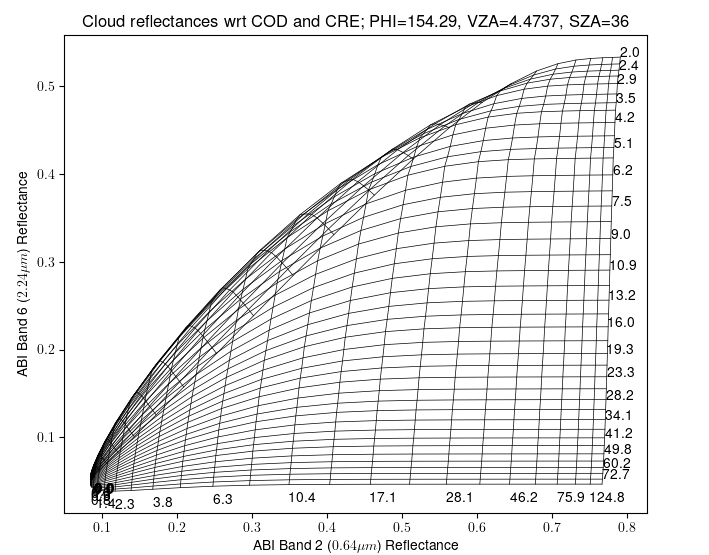
\includegraphics[width=.39\paperwidth]{figs/bispectral_b6.png}
            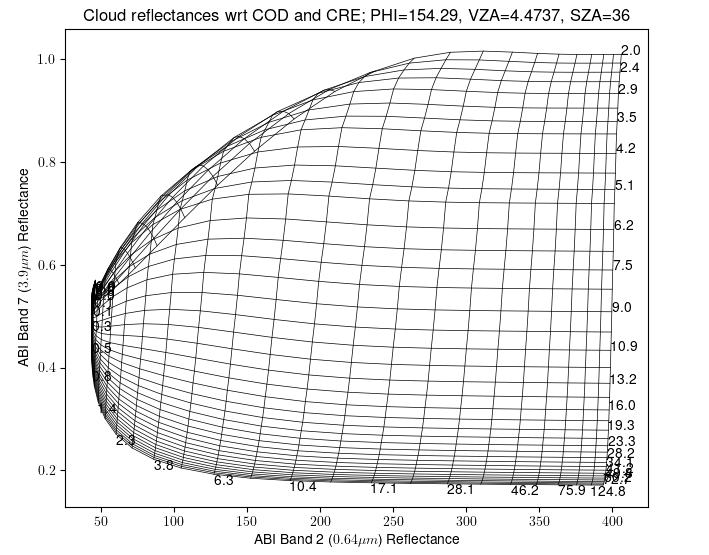
\includegraphics[width=.39\paperwidth]{figs/bispectral_b7.png}
        }

    \end{center}
    \caption{Comparison of lookup table values for absorptive ABI Band 6 ($2.24\mu m$) and Band 7 ($3.9\mu m$), both with respect to conservative-scattering ABI Band 2 ($0.64\mu m$). For sufficiently optically-thick clouds, the increment changes in reflectance per change in COD or CRE are nearly orthogonal to each other, which is the phenomenon exploited by cloud property retrieval as established by (Nakajima and King, 1990) \cite{nakajima_determination_1990}. The reflectance function for water clouds in the $3.9\mu m$ channel is roughly an order of magnitude more sensitive to the effective radius of cloud particles, however thermal emissions play a significant role in observed radiance in this waveband. In order to use the $3.9\mu m$ channel, additional lookup tables for cloud emissivity as a function of COD and CRE would need to be incorporated into the forward model to correct for the emissions. Thus, in order to avoid accruing additional model error and computational cost, I will proceed to only use the $2.24\mu m$ band for the remainder of this project.}
    \label{b6b7_bispec}
\end{figure}

\vspace{-1em}

\section{Retrieval Domain}

\vspace{-2em}

\begin{figure}[h!]
    \centering
    \begin{center}
        \makebox[\textwidth]{
            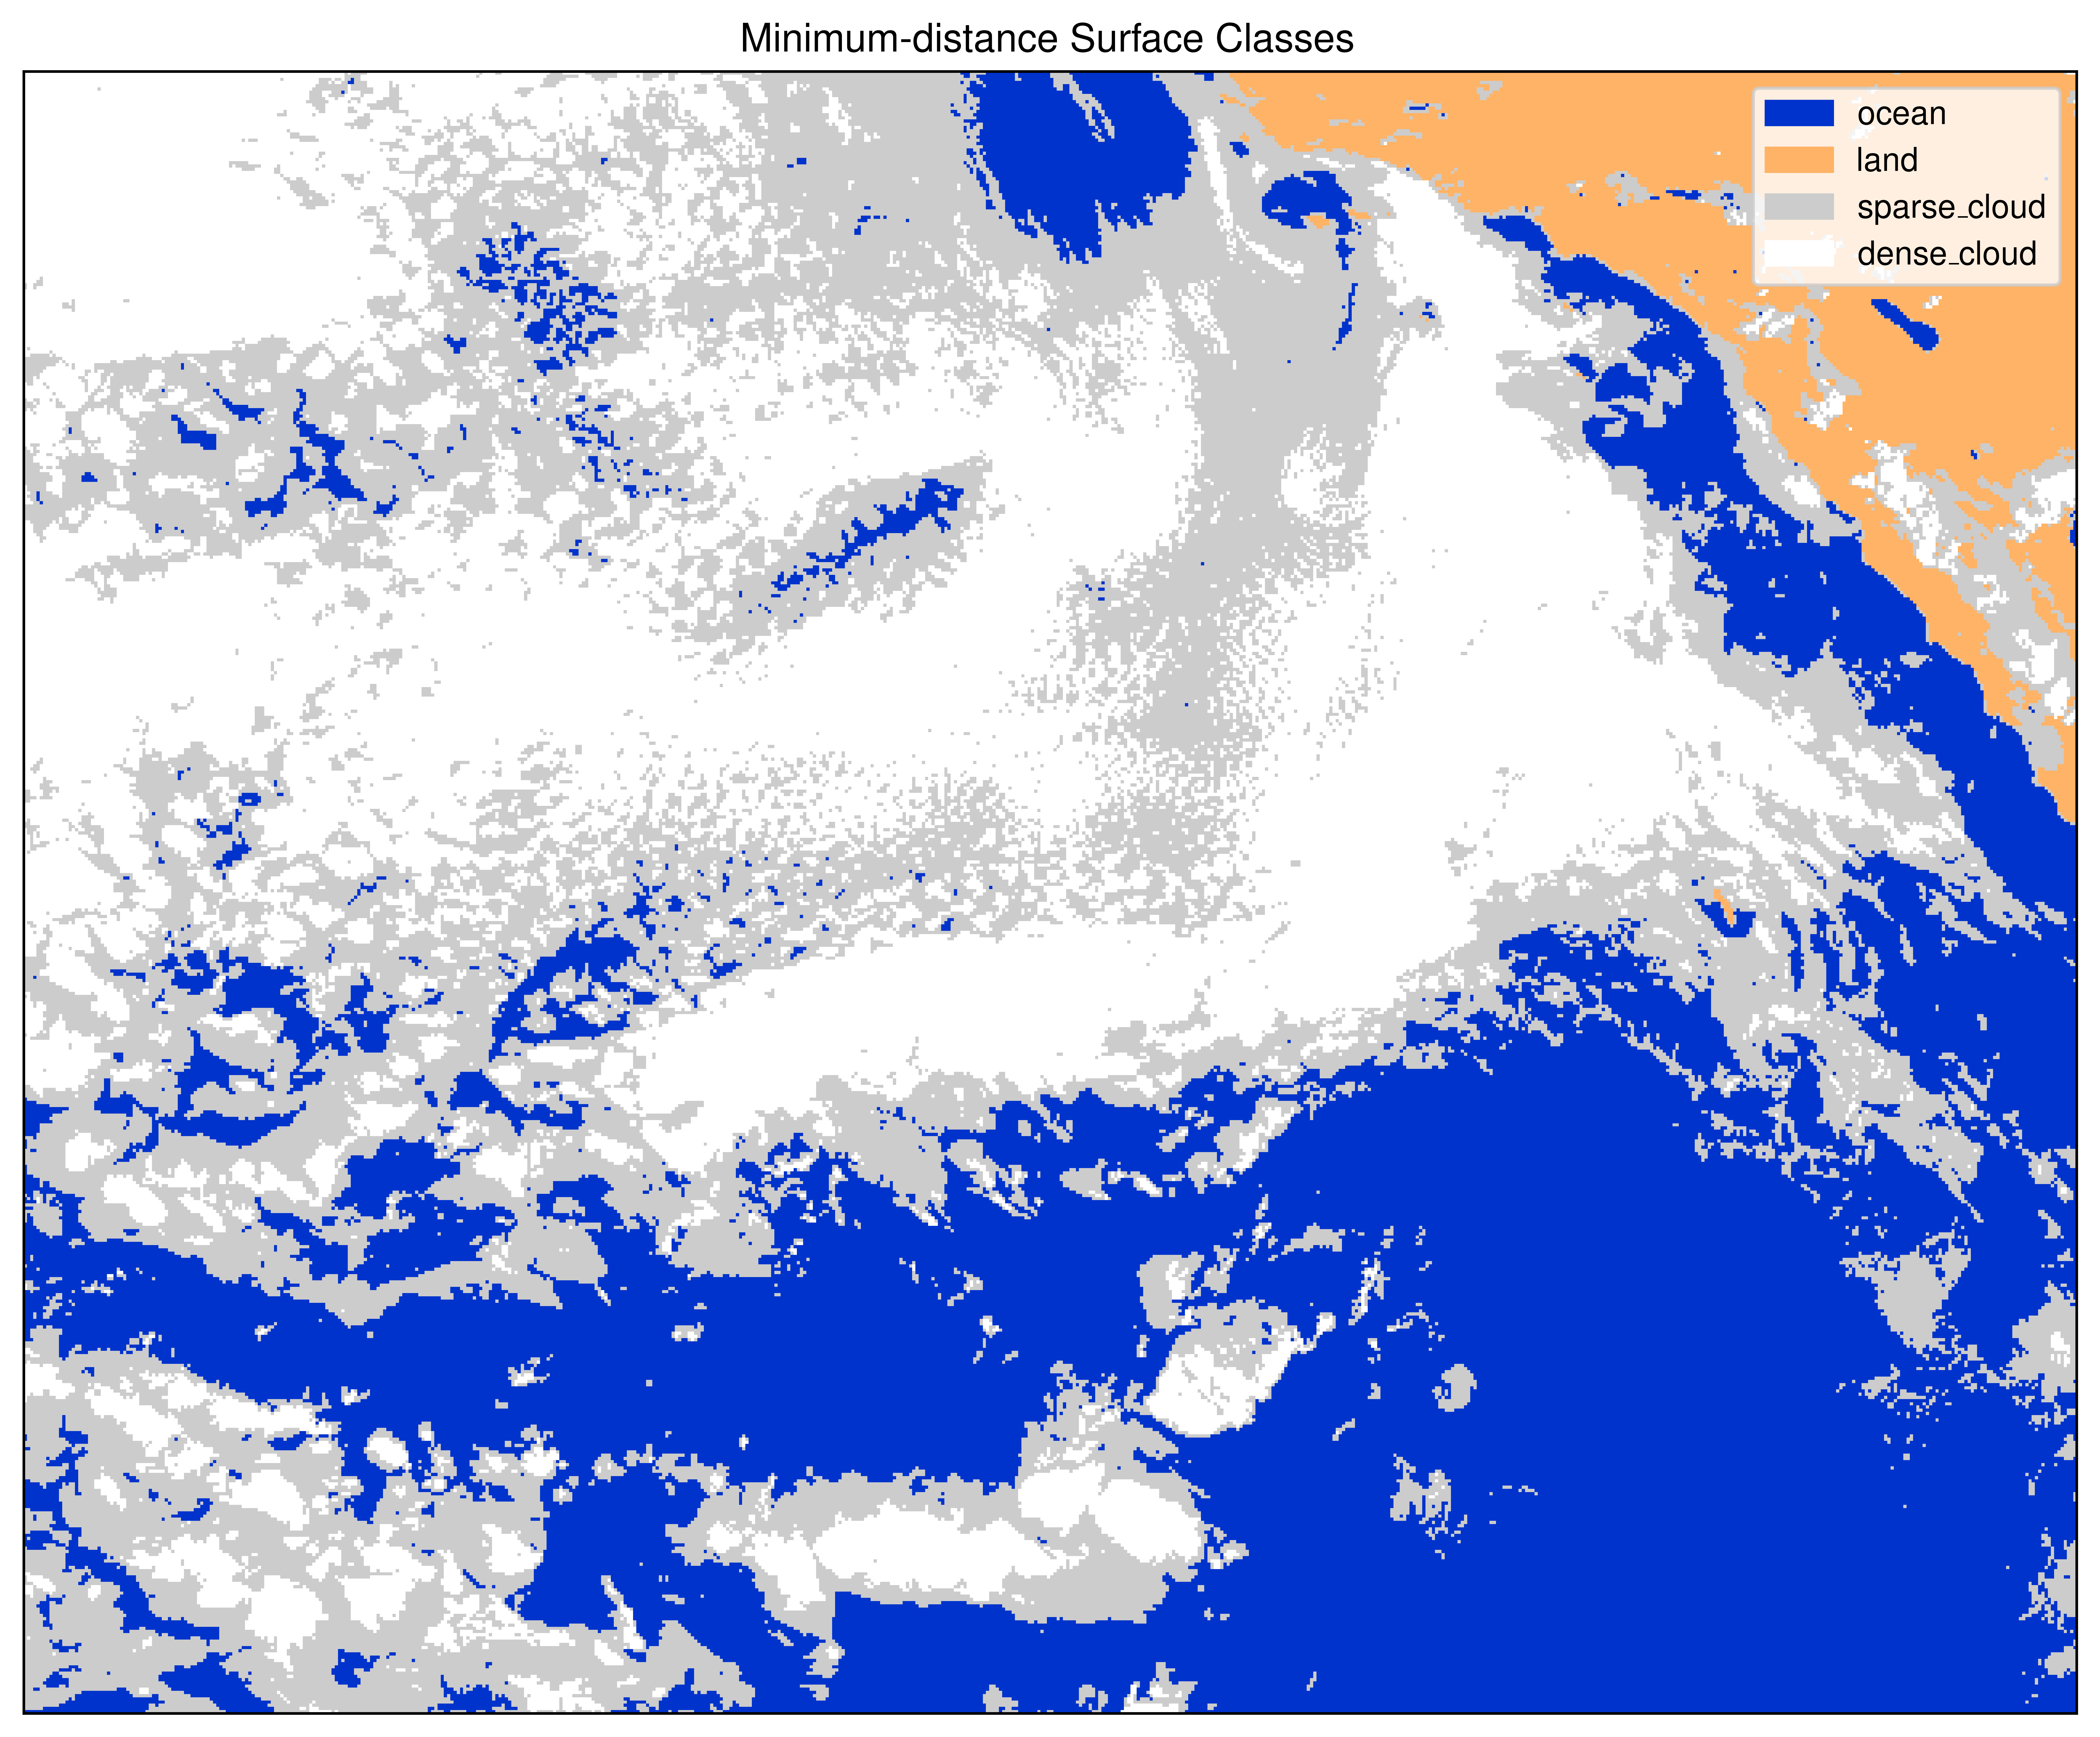
\includegraphics[width=.39\paperwidth]{figs/classes.png}
            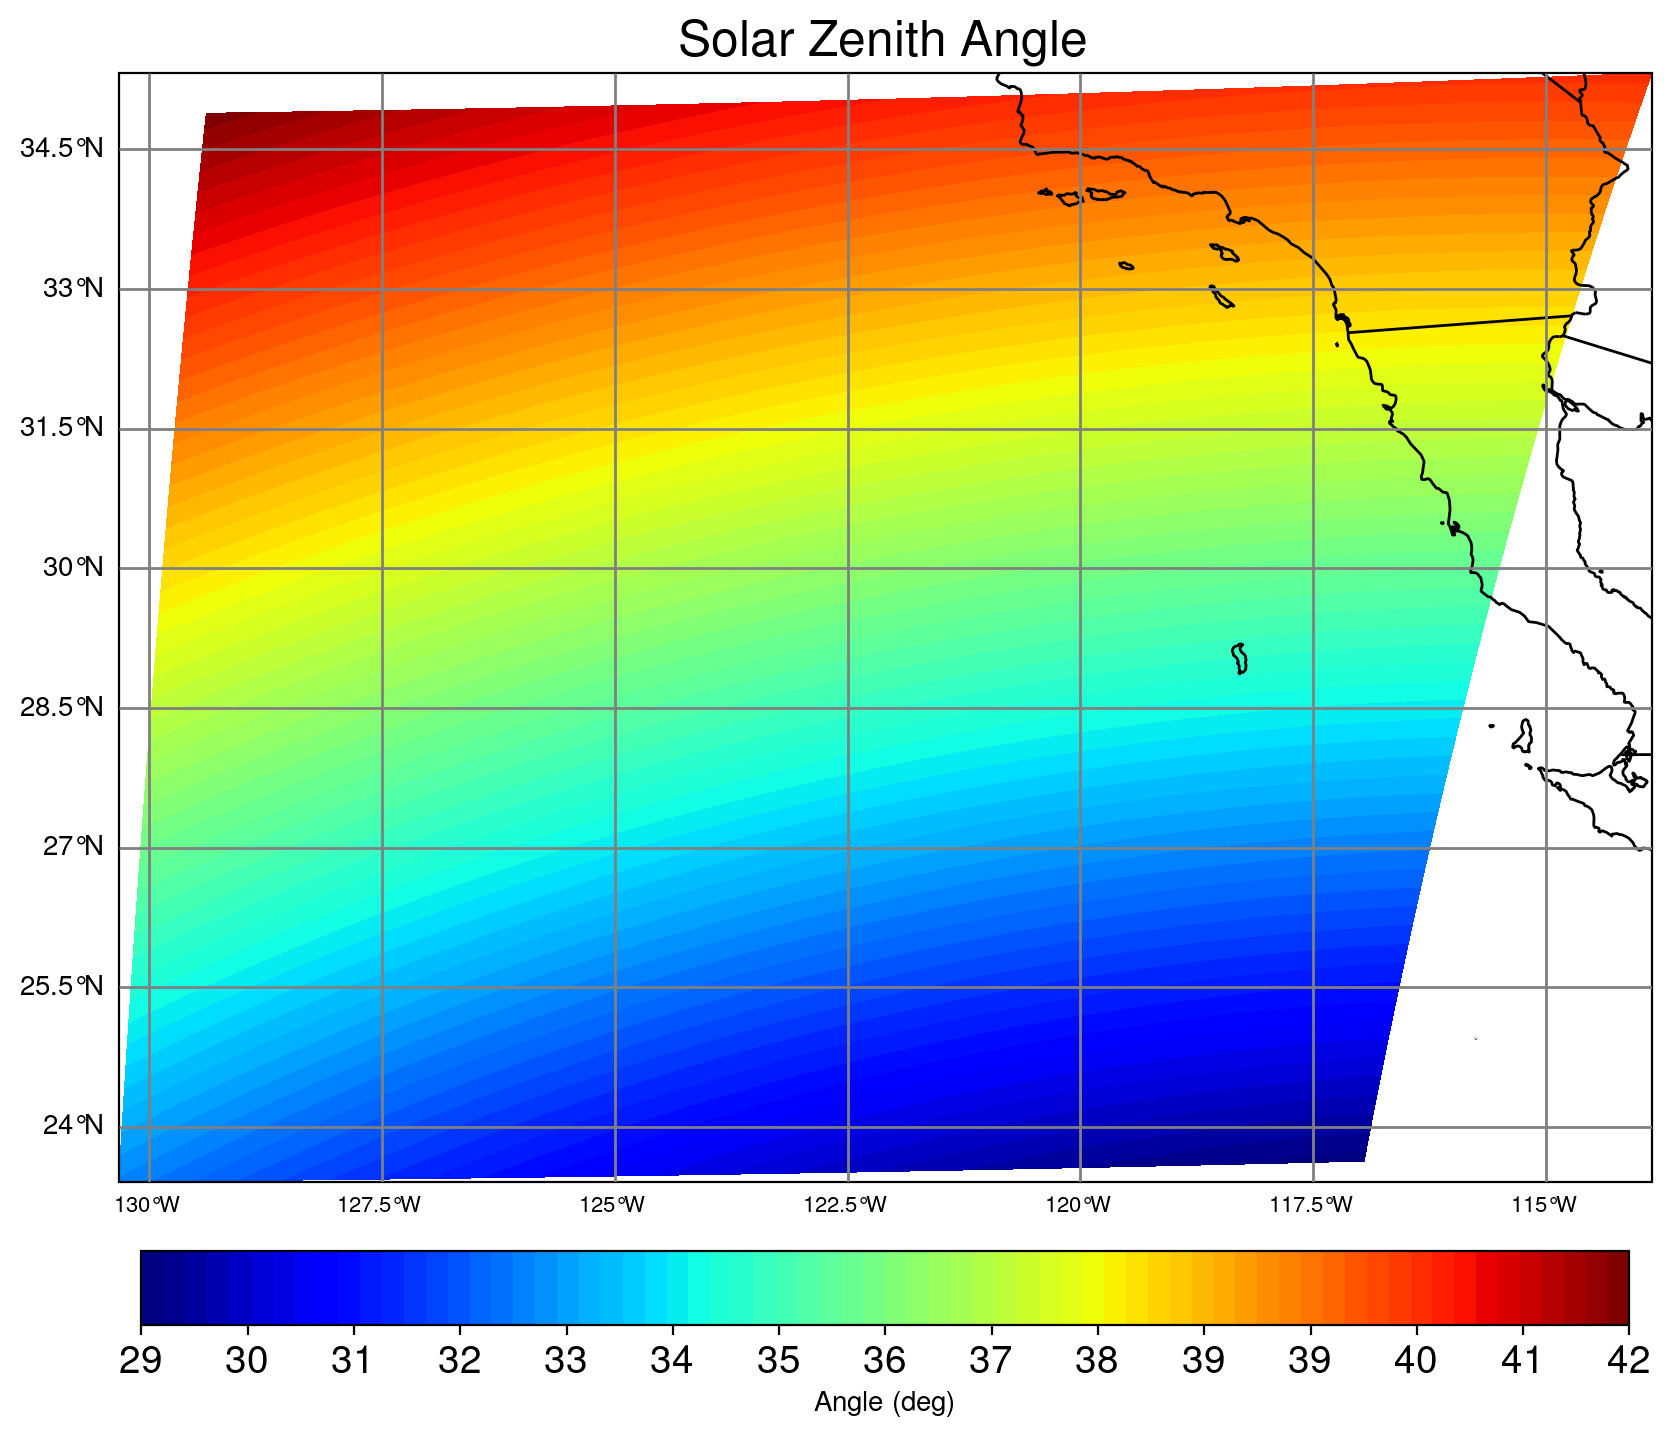
\includegraphics[width=.39\paperwidth]{figs/scal_sza.png}
        }
    \end{center}
    \caption{Minimum-distance surface classes and solar zenith angles over my region. Solar zenith angles over my region are between $29^\circ$ and $43^\circ$, and relative azimuth angles are between $130^\circ$ and $150^\circ$.}
    \label{region_classes}
\end{figure}

\begin{figure}[h!]
    \centering
    \begin{center}
        \makebox[\textwidth]{
            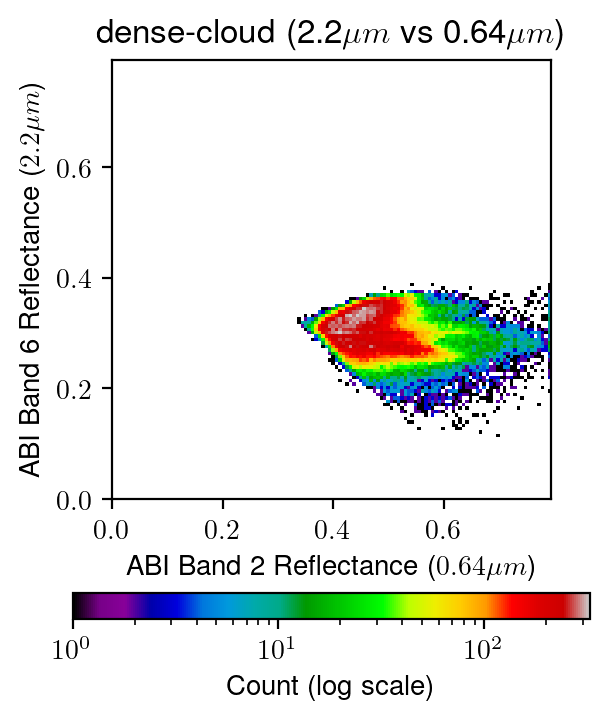
\includegraphics[width=.39\paperwidth]{figs/heatmap_b2b6_dense-cloud.png}
            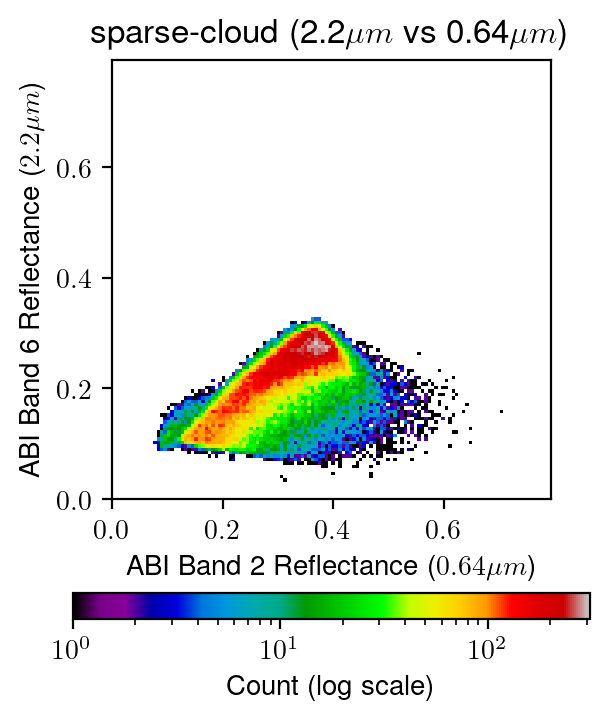
\includegraphics[width=.39\paperwidth]{figs/heatmap_b2b6_sparse-cloud.png}
        }

        \makebox[\textwidth]{
            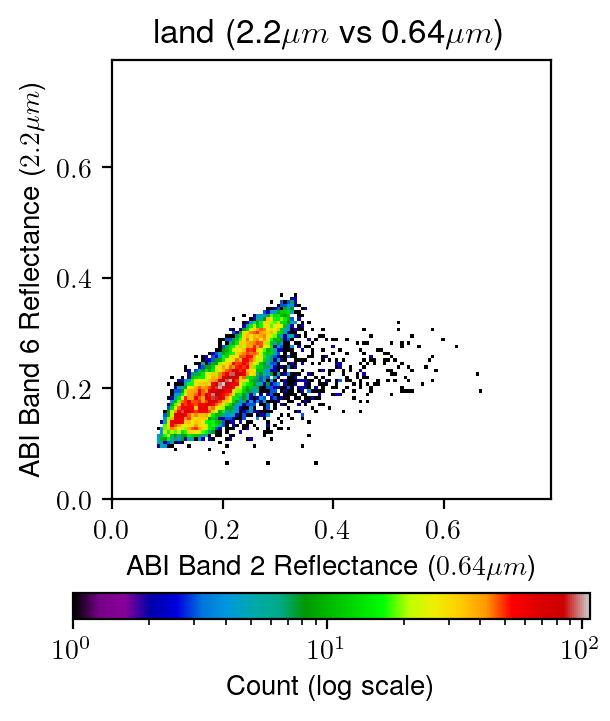
\includegraphics[width=.39\paperwidth]{figs/heatmap_b2b6_land.png}
            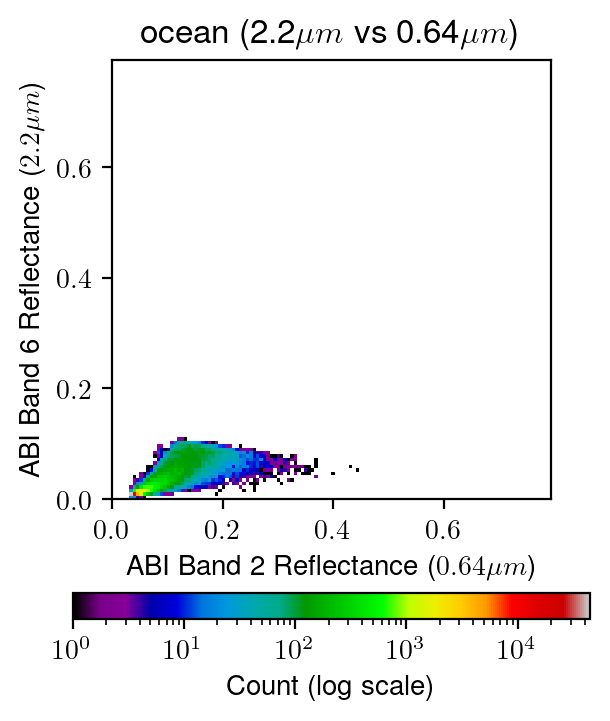
\includegraphics[width=.39\paperwidth]{figs/heatmap_b2b6_ocean.png}
        }
    \end{center}
    \caption{Comparisons of surface types in ABI Band 2 ($0.64\mu m$) and ABI Band 6 ($2.24\mu m$). Top: dense and sparse clouds; bottom: land and ocean. Surfaces were classified using maximum-likelihood classification based on manually-selected pixel samples. Ultimately I performed all retrievals over both dense and sparse cloud surfaces.}
    \label{domain_rgbs}
\end{figure}

\clearpage

\begin{figure}[h!]
    \centering
    \begin{center}
        \makebox[\textwidth]{
            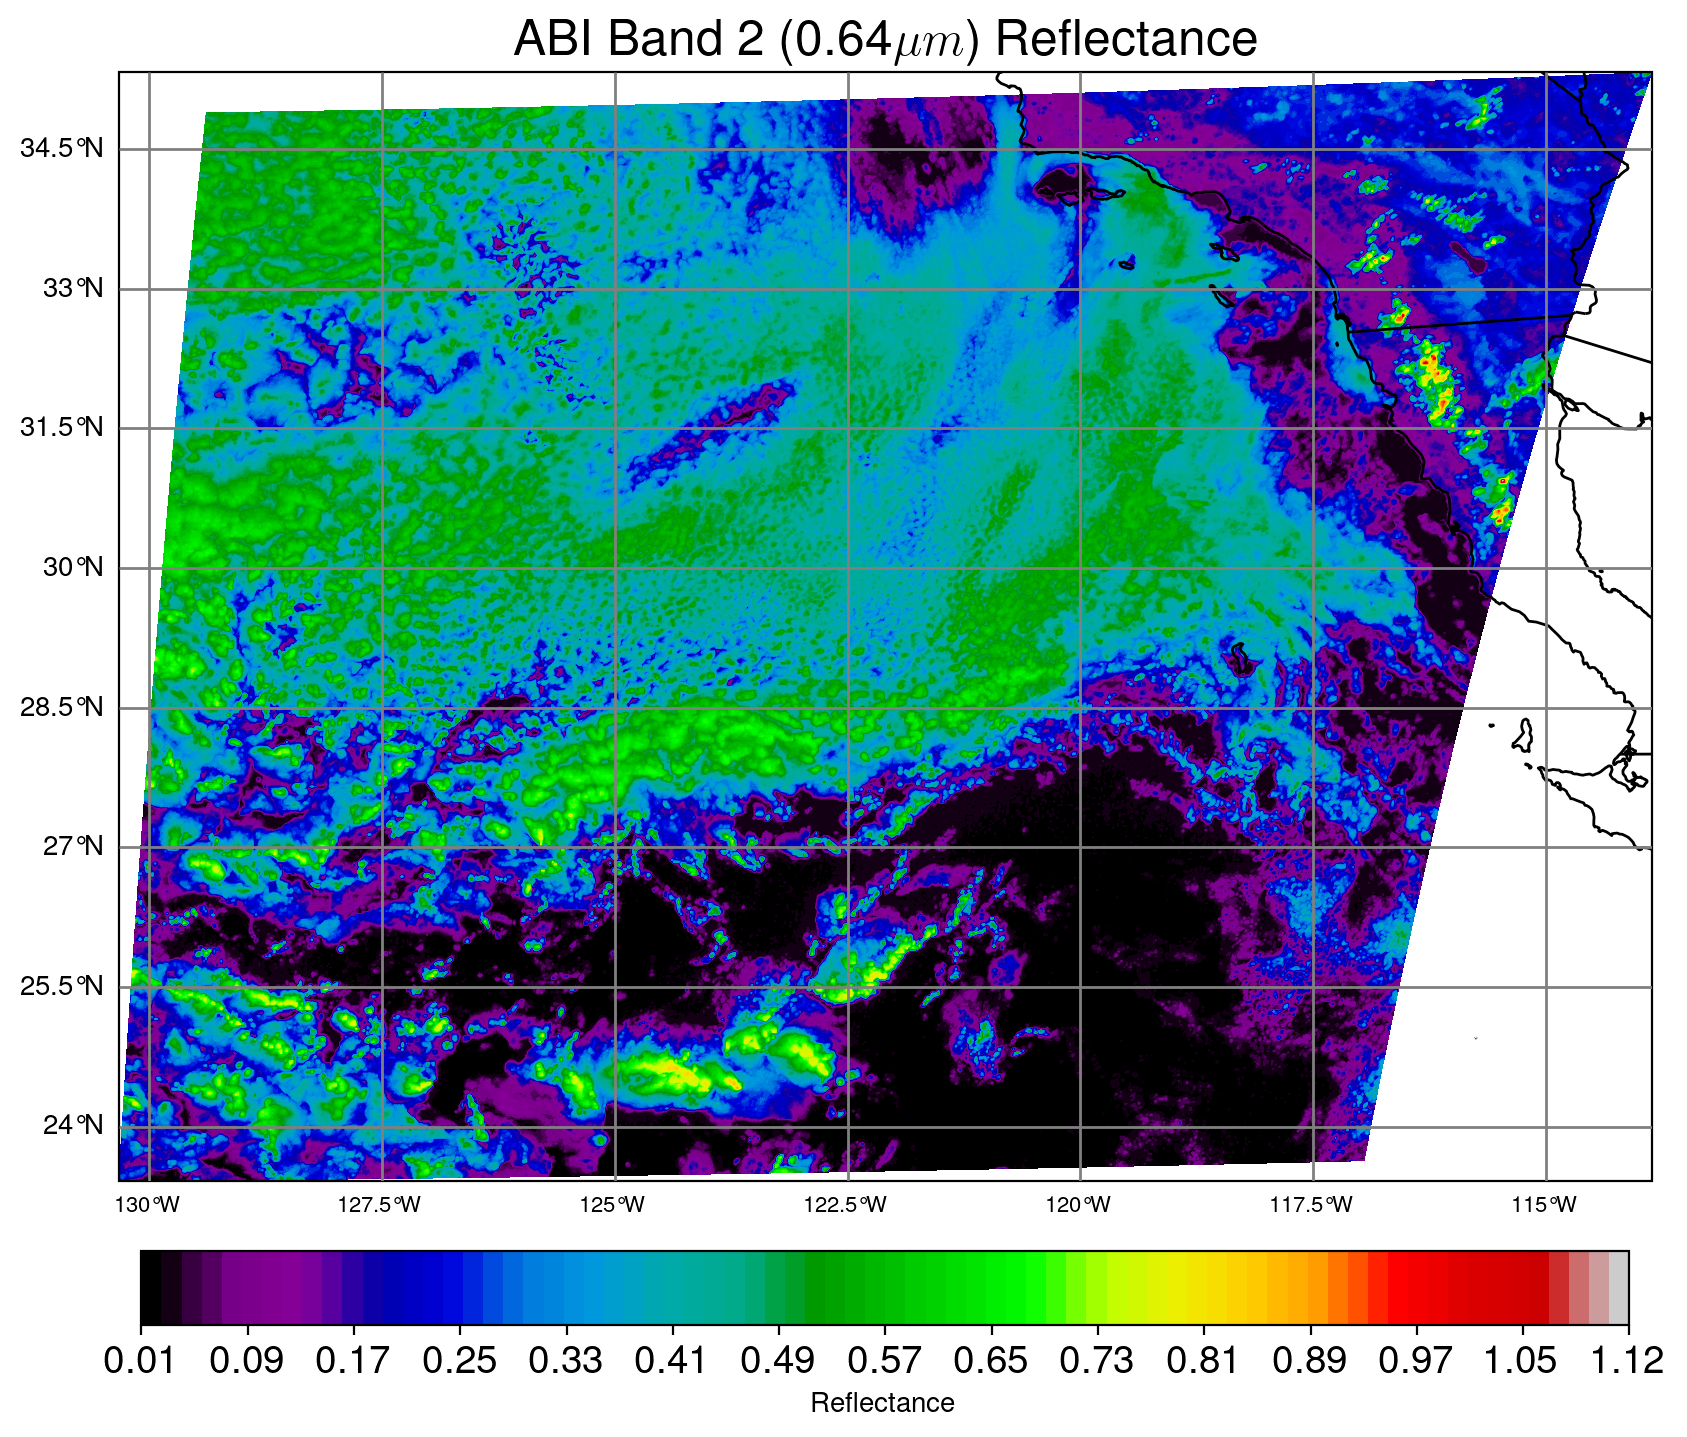
\includegraphics[width=.39\paperwidth]{figs/scal_2-ref.png}
            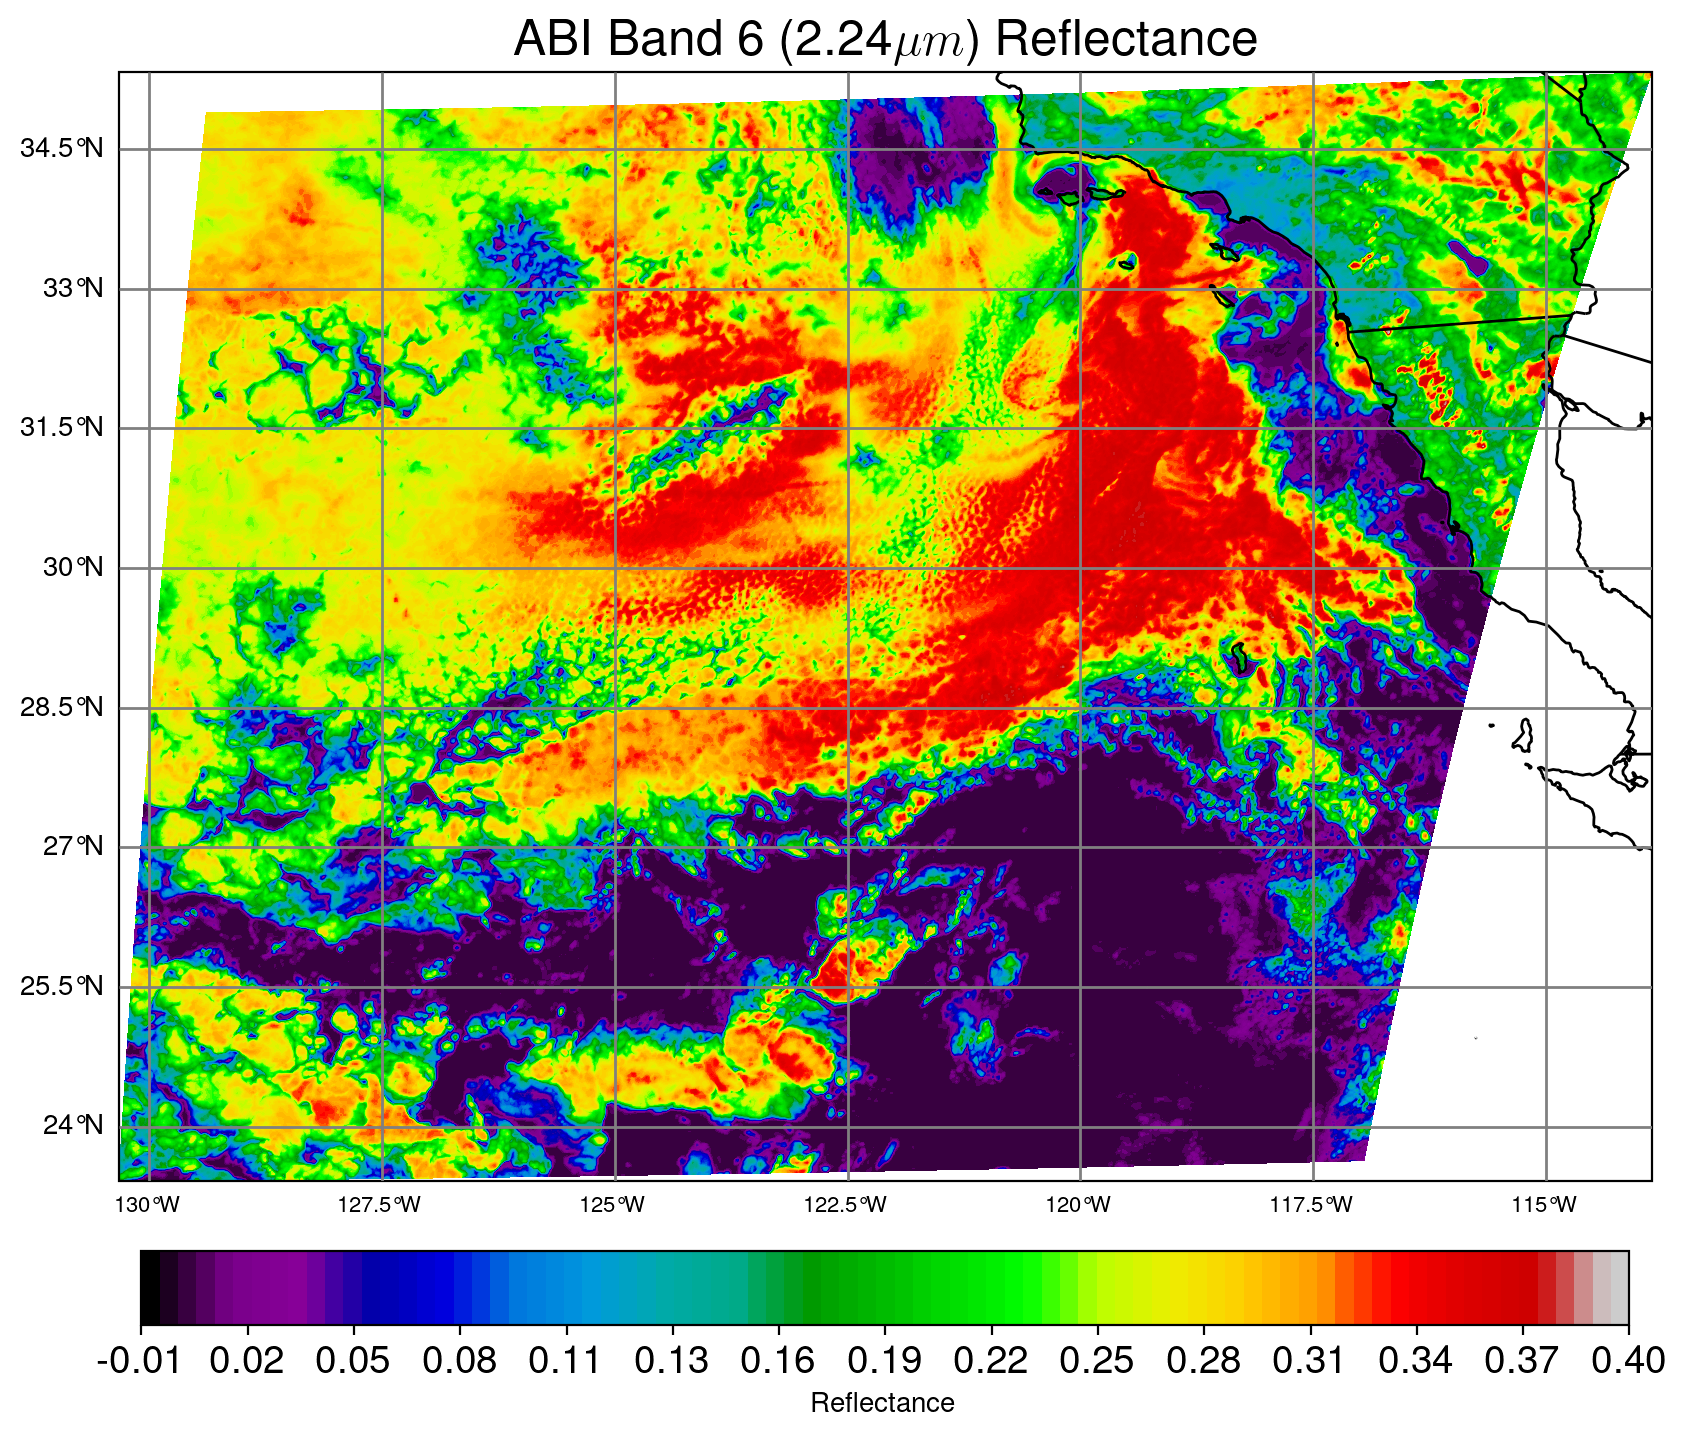
\includegraphics[width=.39\paperwidth]{figs/scal_6-ref.png}
        }
    \end{center}
    \caption{Scalar plots of $0.64\mu m$ reflectance (left), and $2.24\mu m$ reflectance (right). Notice that the color bar scale for the $0.64\mu m$ channel includes values in the range $[0,\,1.2]$, while the $2.24\mu m$ channel only covers values in $[0,\,0.4]$.}
    \label{region_scalars}
\end{figure}

From the images in Figure \ref{region_scalars}, it's visually apparent that the cloud-top features observed in the conservative scattering channel don't strongly correlate with the dominant features of the absorptive band. Since the ocean surface albedo is low, the $0.64\mu m$ channel as a proxy for cloud optical depth such that the thickest clouds are generally those with the highest observed reflectance, which are the bright green nodes in the center and top left of the region, as well as a few deep isolated clouds near the bottom. Ocean surface albedo is especially low in the $2.24\mu m$ channel. Per the bispectral diagrams in Figure \ref{b6b7_bispec}, the cloud-top reflectivity function in this channel increases as CRE decreases. As such, the observations suggest that the finest particles are found in the stratiform region extending from the California coastline into the center of the region. In terms of physical rationalization, I suspect that this cloud region corresponds to the newest clouds condensing due to the sea breeze, which may have a generally finer distribution of droplet sizes since the cloud layer has had less time to coagulate into larger particles.

\section{Retrieval Procedure}

\subsection{Mathematical Background}

\begin{equation}\label{chi2}
    \chi^2 = \left(\ln{R^{(VIS)}_{obs}}-\ln{R^{(VIS)}_{fwd}}\right)^2 + \left(\ln{R^{(NIR)}_{obs}}-\ln{R^{(NIR)}_{fwd}}\right)^2
\end{equation}

Having generated all needed lookup tables and defined the clouded area of regard, I implemented an Optimal Estimate Inversion algorithm similar to the procedure outlined in the ABI DCOMP algorithm theoretical basis document from the GOES-R Algorithm Working Group \cite{uw_algorithm_nodate}. This technique regards the cloud properties $\tau_c$ and $r_e$ as a 2-element state vector parameterizing a chi-squared distribution of the form outlined in Equation \ref{chi2}, which accounts for the difference between forward-model ($R_{fwd}$) and observed ($R_{obs}$) reflectances in both the visible and near-infrared channels. If the forward-function were analytic, the process of finding a $[\tau_c, r_e]$ state that best fits the data would involve solving for the minima of the gradient of Equation \ref{chi2} with respect to the state on a per-pixel basis.

\begin{equation}\label{dcomp_cost}
    d^2_i = \left[\vec{x}_i-\vec{x}_{i+1}\right]^TS_x^{-1}\left[\vec{x}_i-\vec{x}_{i+1}\right]
\end{equation}

\begin{equation}\label{walther_cost}
    J = \left[\vec{y}-F(\vec{x})\right]^TS_y^{-1}\left[\vec{y}-F(\vec{x})\right] + \left[\vec{x}_a - \vec{x}\right]^T S_a^{-1} \left[\vec{x}_a - \vec{x}\right]
\end{equation}

Since in this case we must rely on discrete lookup tables as a forward function, the state needs to be solved for iteratively for each pixel by optimizing a well-defined cost function that both (1) approximates the $\chi^2$ goodness-of-fit and (2) takes into consideration error in the observation quality, a-priori state, and the forward model uncertainty. In general, optimization entails starting with an a-priori guess for the state, using a transition function to determine a new state, and continuing to re-evaluate it until a stopping criterion is achieved.

The DCOMP ATBD employs the cost function specified in Equation \ref{dcomp_cost} with the stopping condition that either $d^2 < 1$ or a user-specified maximum number of iterations are performed \cite{uw_algorithm_nodate}. Equation \ref{walther_cost} is an alternative form of the same expression, which is used by the same authors in (Walther and Heidinger, 2012), though without specifying a stopping condition. \cite{walther_implementation_2012} In these equations, $\vec{x}$ is the state vector $[\tau_c, r_e]$, $\vec{y}$ is the observed reflectance $[R^{(VIS)}, R^{(NIR)}]$, and $F(\vec{x})$ is the forward-model reflectance given the current state $\vec{x}$.

\begin{equation}\label{err_mats}
    \begin{split}
        S_a &:= \begin{pmatrix}\sigma^2_{\tau, a} & 0 \\ 0 & \sigma^2_{r_e, a}\end{pmatrix} \\
            & \approx \begin{pmatrix} .04 & 0 \\ 0 & .25\end{pmatrix} \\
        S_y &:= \begin{pmatrix}\sigma^2_{VIS, a} & 0 \\ 0 & \sigma^2_{NIR, a}\end{pmatrix} \\
            &\approx \begin{pmatrix} 0.16\cdot R^{(VIS)}+0.02 & 0 \\ 0 & 0.16\cdot R^{(NIR)}+0.02\end{pmatrix} \\
        S_x &:= \left(S_a^{-1} + K^TS_y^{-1}K\right)^{-1}
    \end{split}
\end{equation}

Equation \ref{err_mats} defines error covariance matrices $S_a$, $S_y$, and $S_x$ which correspond to a-priori uncertainty, observation uncertainty, and model uncertainty, respectively. The specified values for $S_a$ and $S_y$ were gleaned from the DCOMP ATBD and, ironically, were themselves a source of considerable uncertainty in my retrieval process since (1) my forward-model lookup tables and, by extension, a-priori state guesses are different than those used in DCOMP and (2) the matrices appear in every cost metric and, as such, are fundamental for determining the stopping condition.

\begin{equation}\label{jac}
        K := \begin{pmatrix} \frac{\partial R^{(VIS)}}{\partial \tau_c} & \frac{\partial R^{(VIS)}}{\partial r_e} \\ \frac{\partial R^{(NIR)}}{\partial \tau_c} & \frac{\partial R^{(NIR)}}{\partial r_e} \end{pmatrix}
\end{equation}
\begin{equation}\label{del}
        \delta \vec{x} := S_x\left(K^T S_y^{-1} (\vec{y}-F(\vec{x})) + S_a^{-1}(\vec{x}_a-\vec{x})\right)
\end{equation}

Equations \ref{jac} and \ref{del} are the expressions for the jacobian matrix and state transition vector provided a pixel observation and current state, which are calculated for every pixel at each iterative step until arriving at a stopping condition.

\subsection{Retrieval Algorithm}\label{dcomp_algo}

\noindent
For each pixel identified as a cloud...
\begin{enumerate}
    \item Set the prior for effective radius to the closest lookup table value to $r_{e,a} = 10\mu m$, then choose the prior optical depth in the corresponding row that is closest to the observed reflectance.
    \item Extract the lookup table entries closest to the current solar zenith, viewing zenith, and relative azimuth angles.
    \item Establish the $S_y$ and $S_a$ matrices for the current pixel observation.
    \item Until the maximum number of iterations is reached, or the current stopping condition is met...
        \begin{enumerate}[label*=\arabic*.]
            \item Identify lookup table values that span the previous state (or a-priori state at the first step).
            \item Calculate the jacobian matrix $K$ in terms of the partial change in forward-model radiance with respect to the surrounding grid points.
            \item Get the offset from the previous state to the lower-bound lookup table point ($\tau_c$ and $r_e$).
            \item Use the new jacobian and offset to estimate the new radiance.
            \item Convert the new radiance as well as the jacobian to reflectance.
            \item Establish $S_x$ using the new jacobian matrix, and use it to calculate the state transition vector $\delta \vec{x}$.
            \item Determine the new state using the transition vector, and use it to evaluate the cost function.
            \item Use the cost function to decide whether to keep the new state, or to stop iteration and revert to the previous state.
        \end{enumerate}
    \item Return the latest state if it was successfully converged upon, or else return a null value if the maximum number of iterations was exceeded.
\end{enumerate}

\section{Retrieval Results}

\subsection{Challenges With A-Priori Values}

In the process of developing my retrievals I encountered considerable difficulty enabling pixel states to escape the a-priori values set by step 1 of the process outlined in the previous section, as Figure \ref{bad_retrievals} makes clear. For the first several runs, the observed effective radius remained within a couple of micrometers of the initial $10\mu m$ guess, and the reflectance-dependent a-priori guesses for optical depth varied little from the discrete grid points used in the lookup table. I attempted retrievals using many different combinations of stopping conditions, covariance matrices, and iteration limits, initially to no avail. For most combinations, a value was returned after less than 5 iterations for $60-70\%$ of pixels, the remainder of which tended to saturate at the maximum number of iterations.

\begin{figure}[h!]
    \centering
    \begin{center}
        \makebox[\textwidth]{
            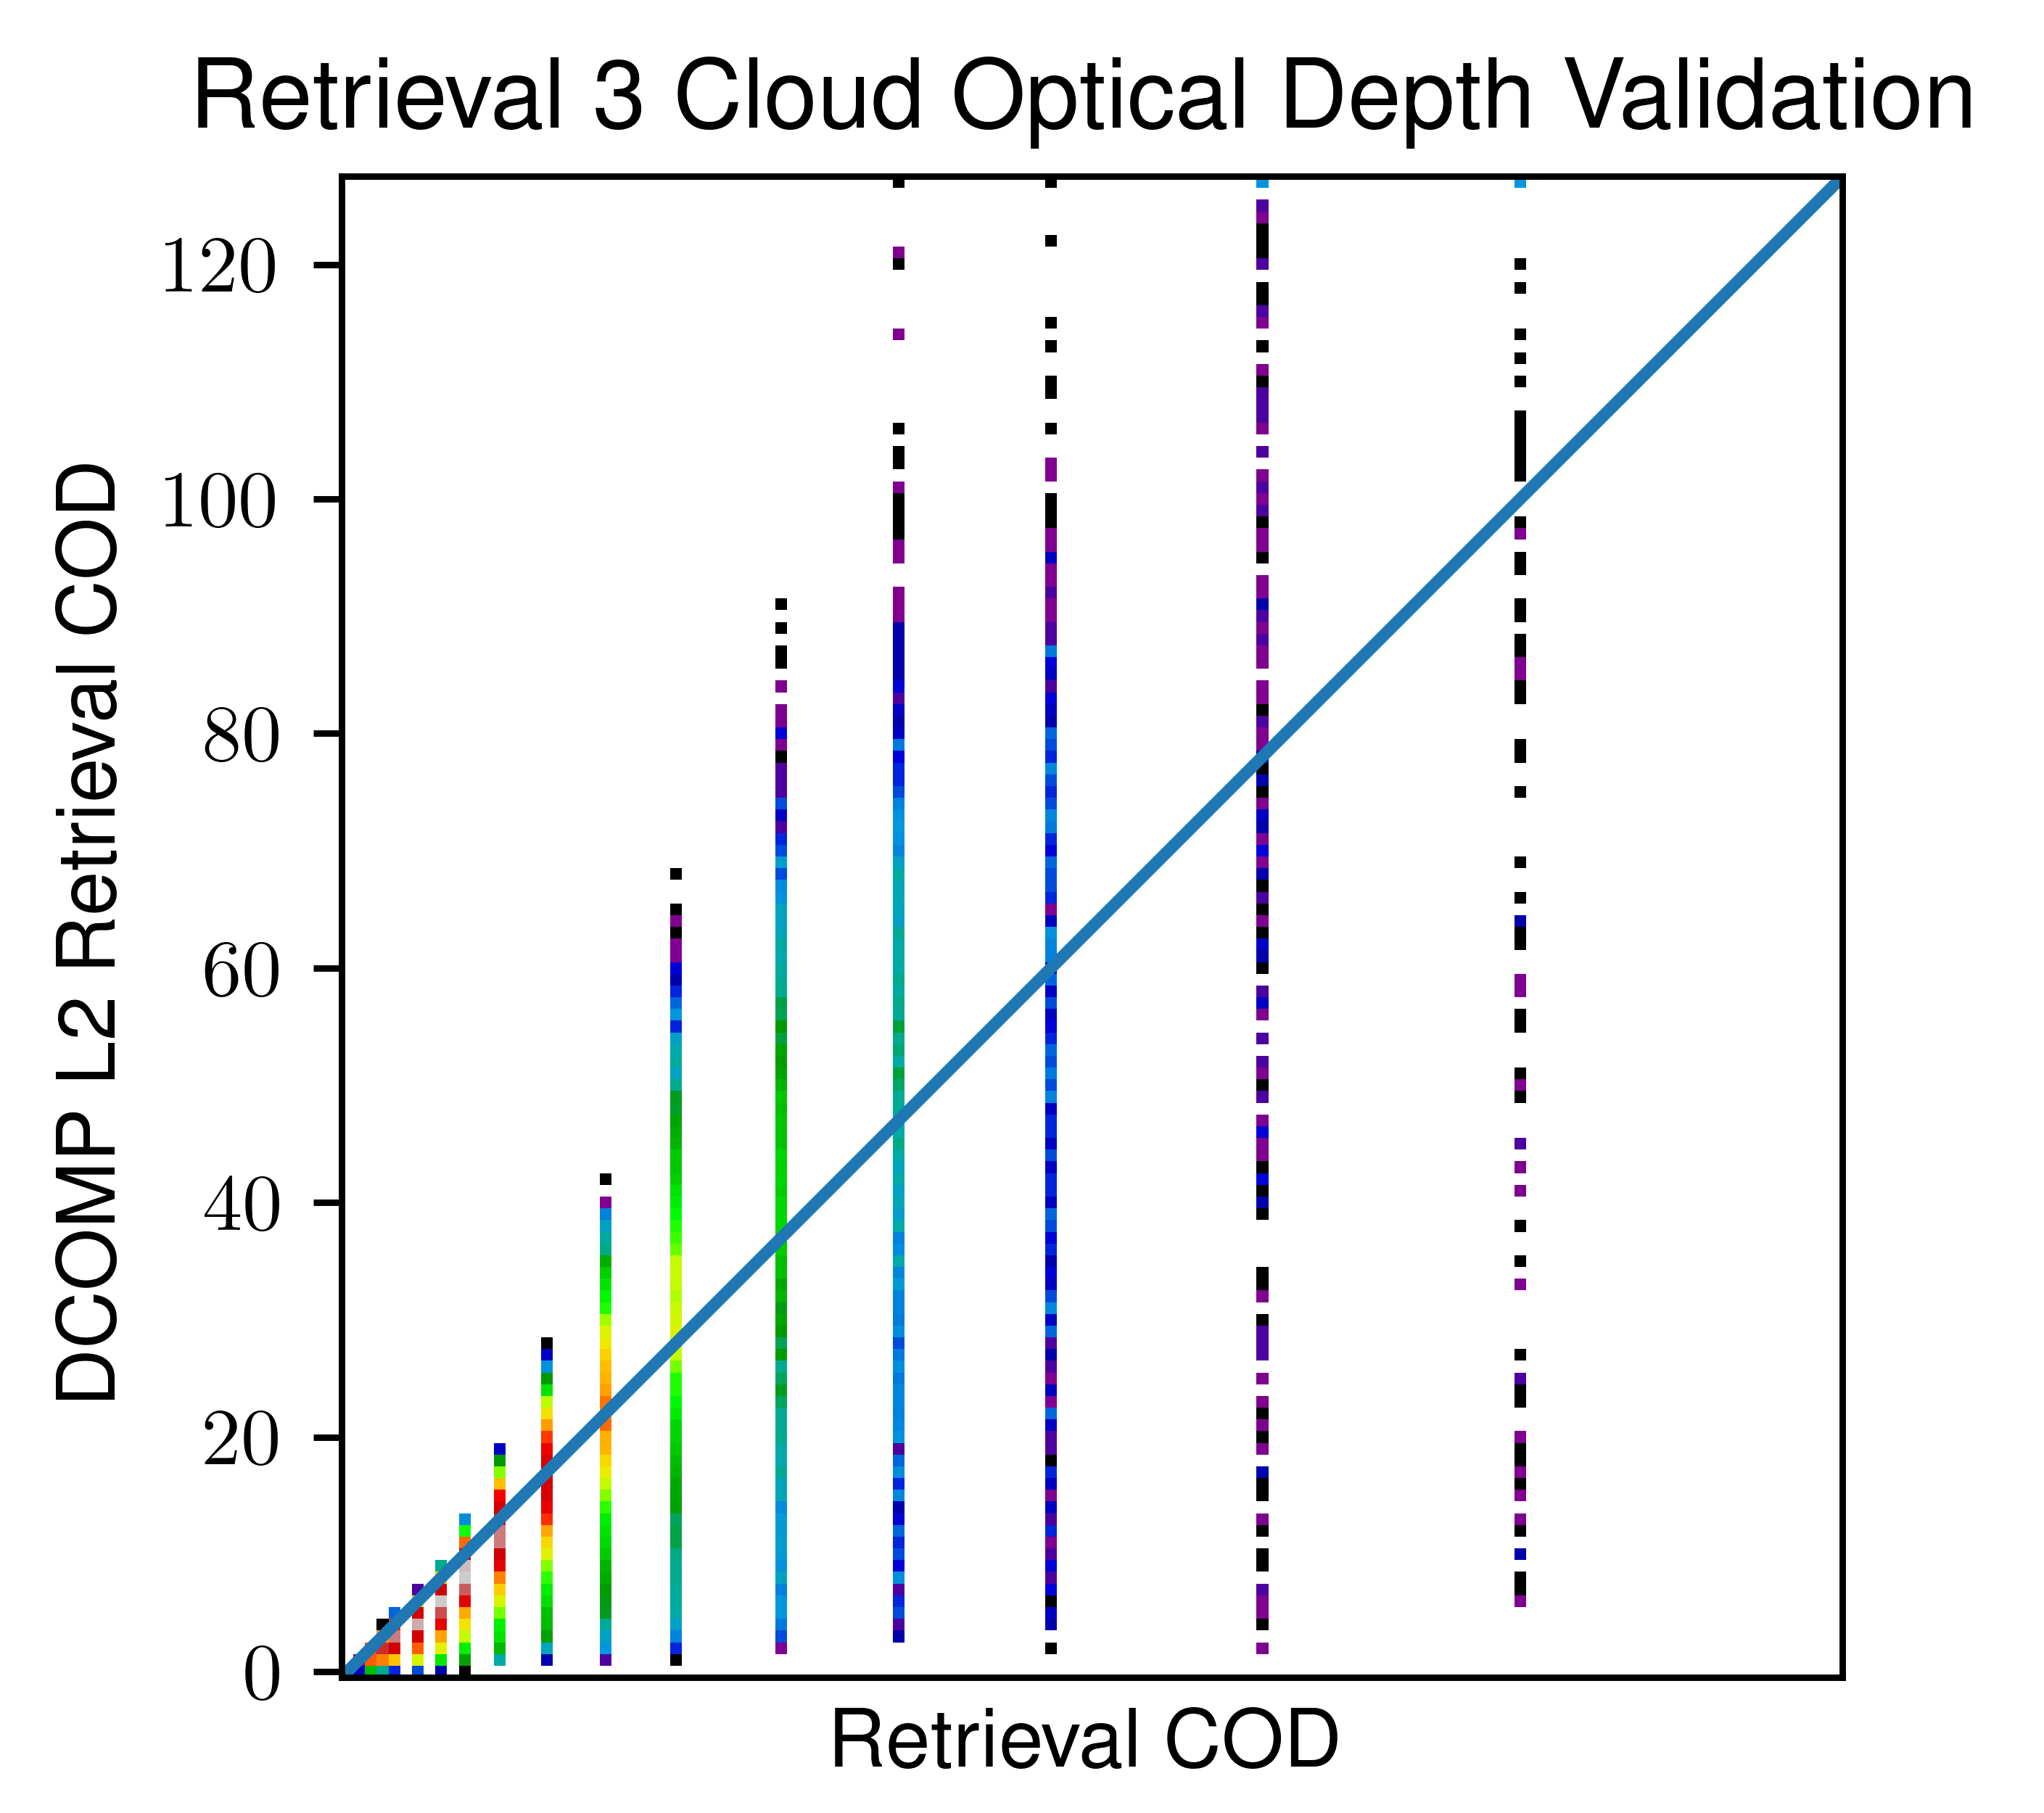
\includegraphics[width=.32\paperwidth]{figs/val_ret3_cod.png}
            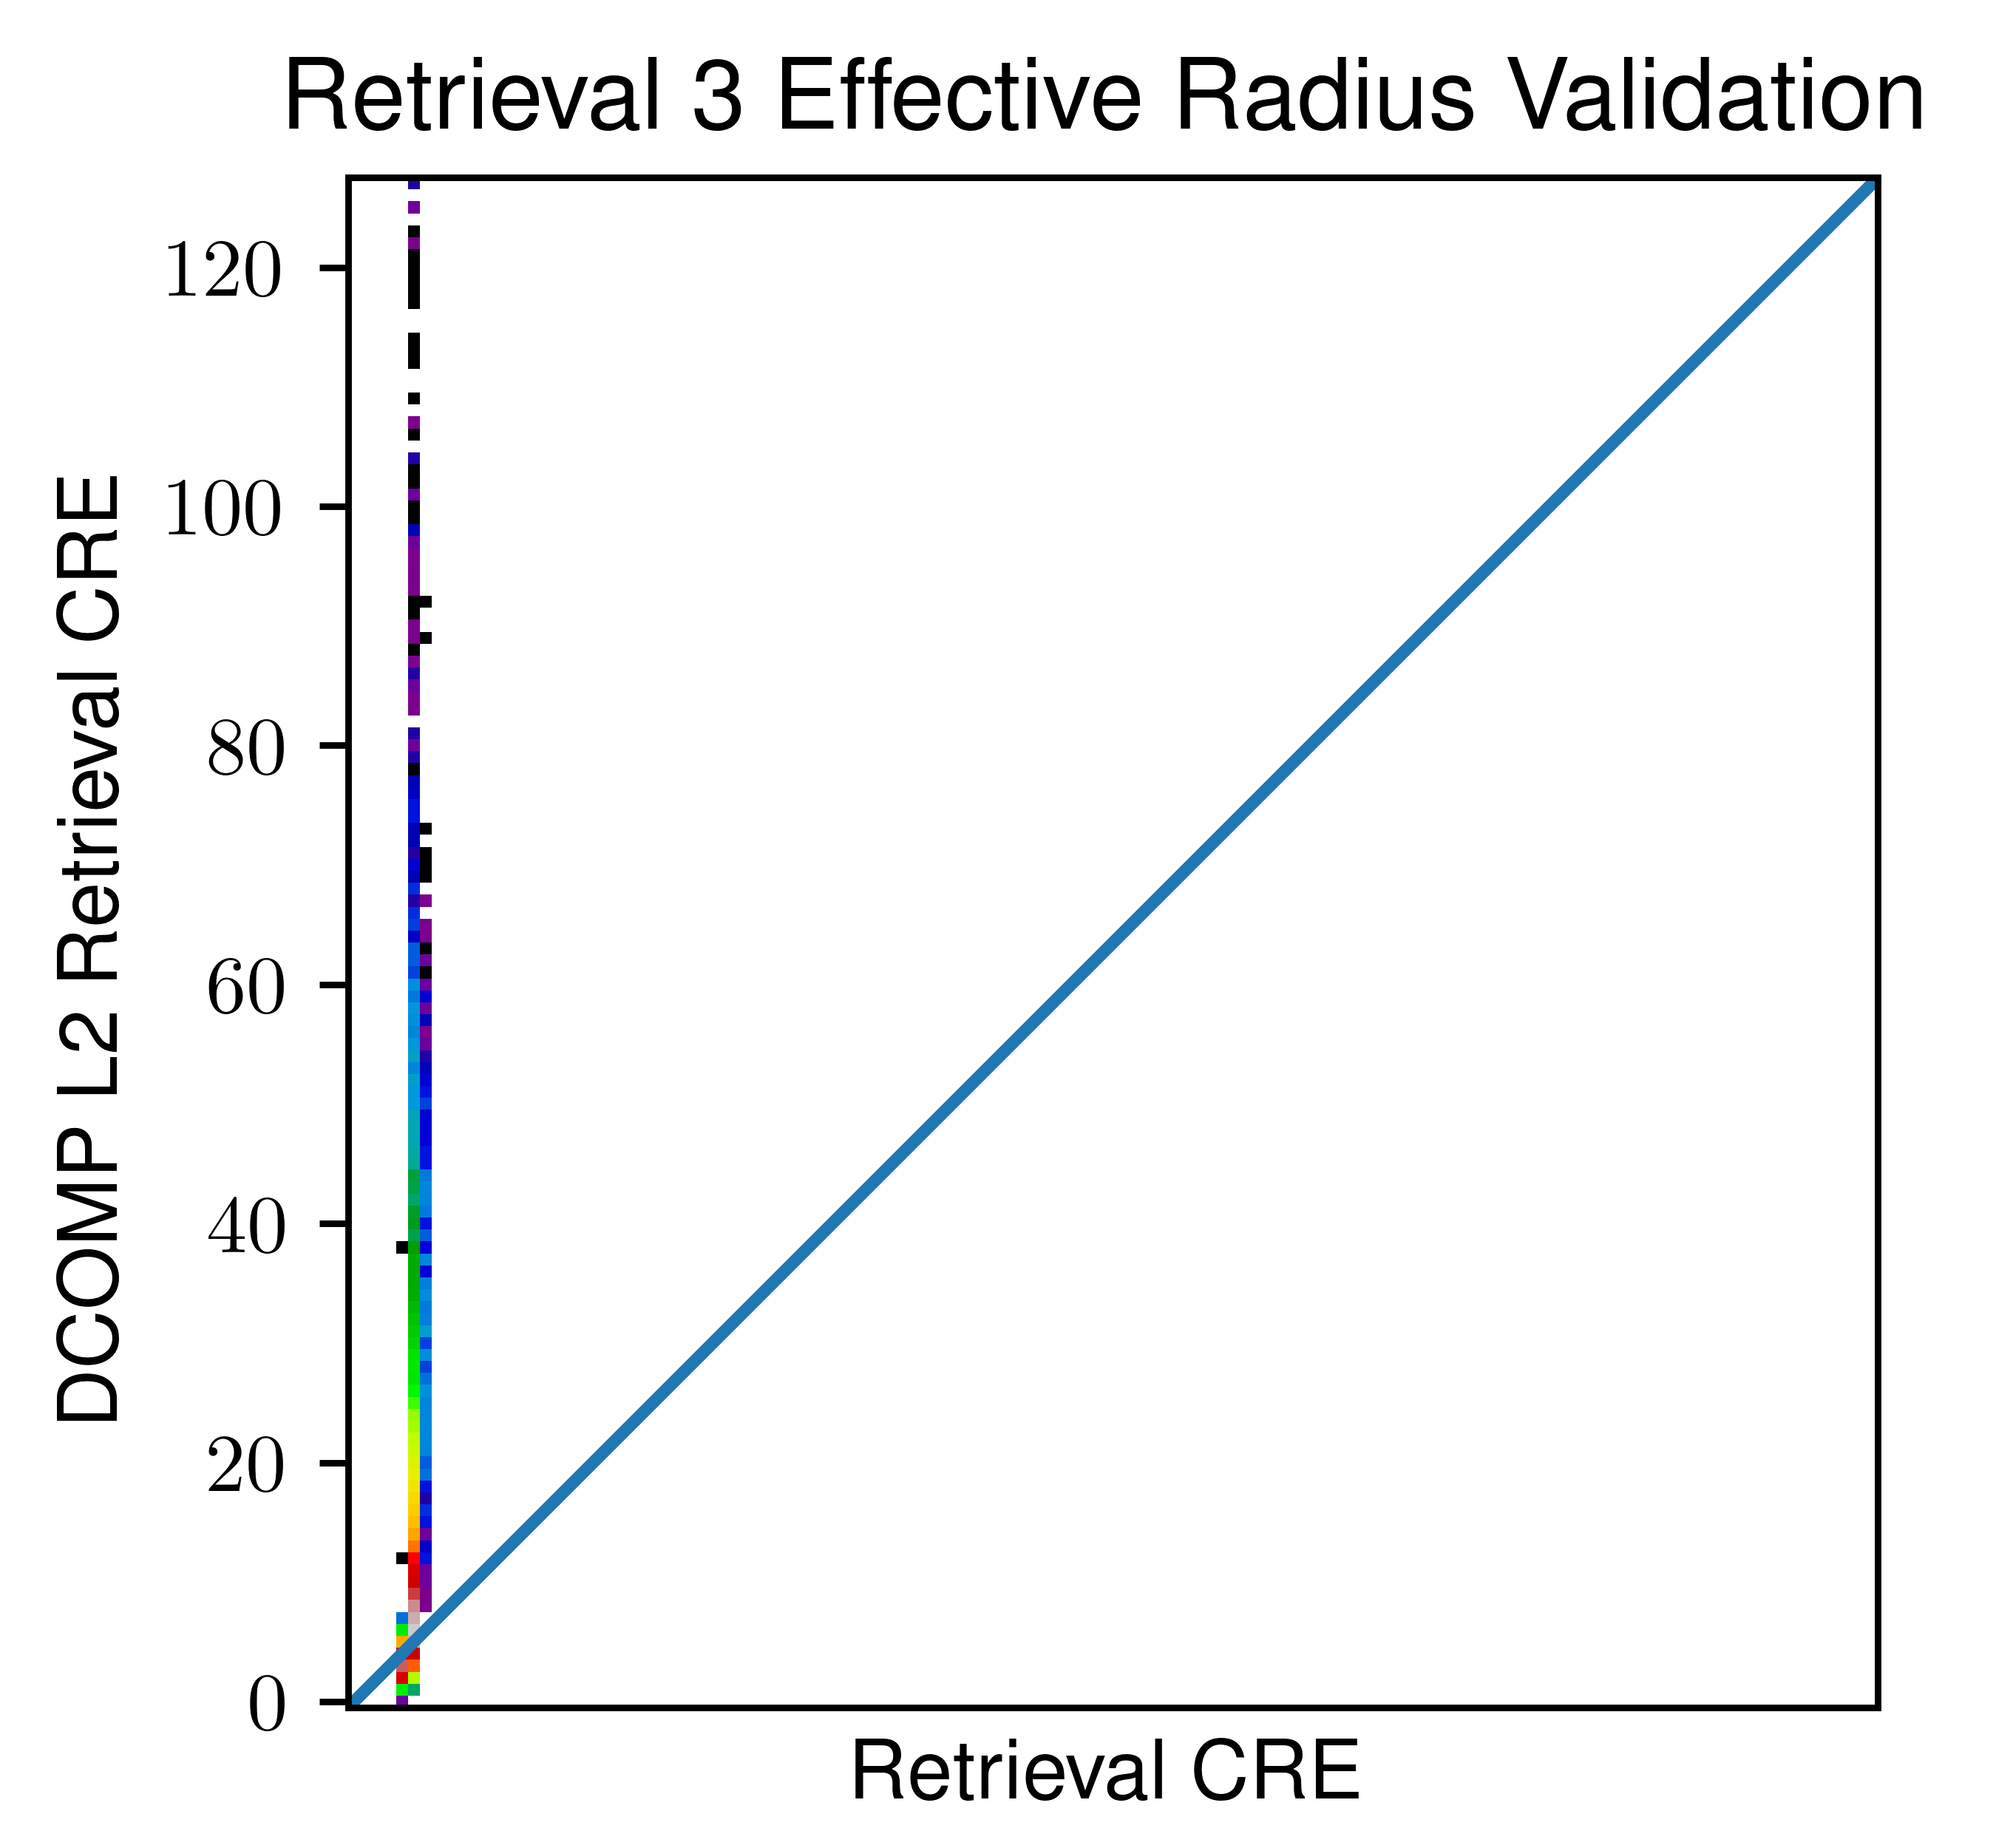
\includegraphics[width=.30\paperwidth]{figs/val_ret3_cre.png}
        }
        \makebox[\textwidth]{
            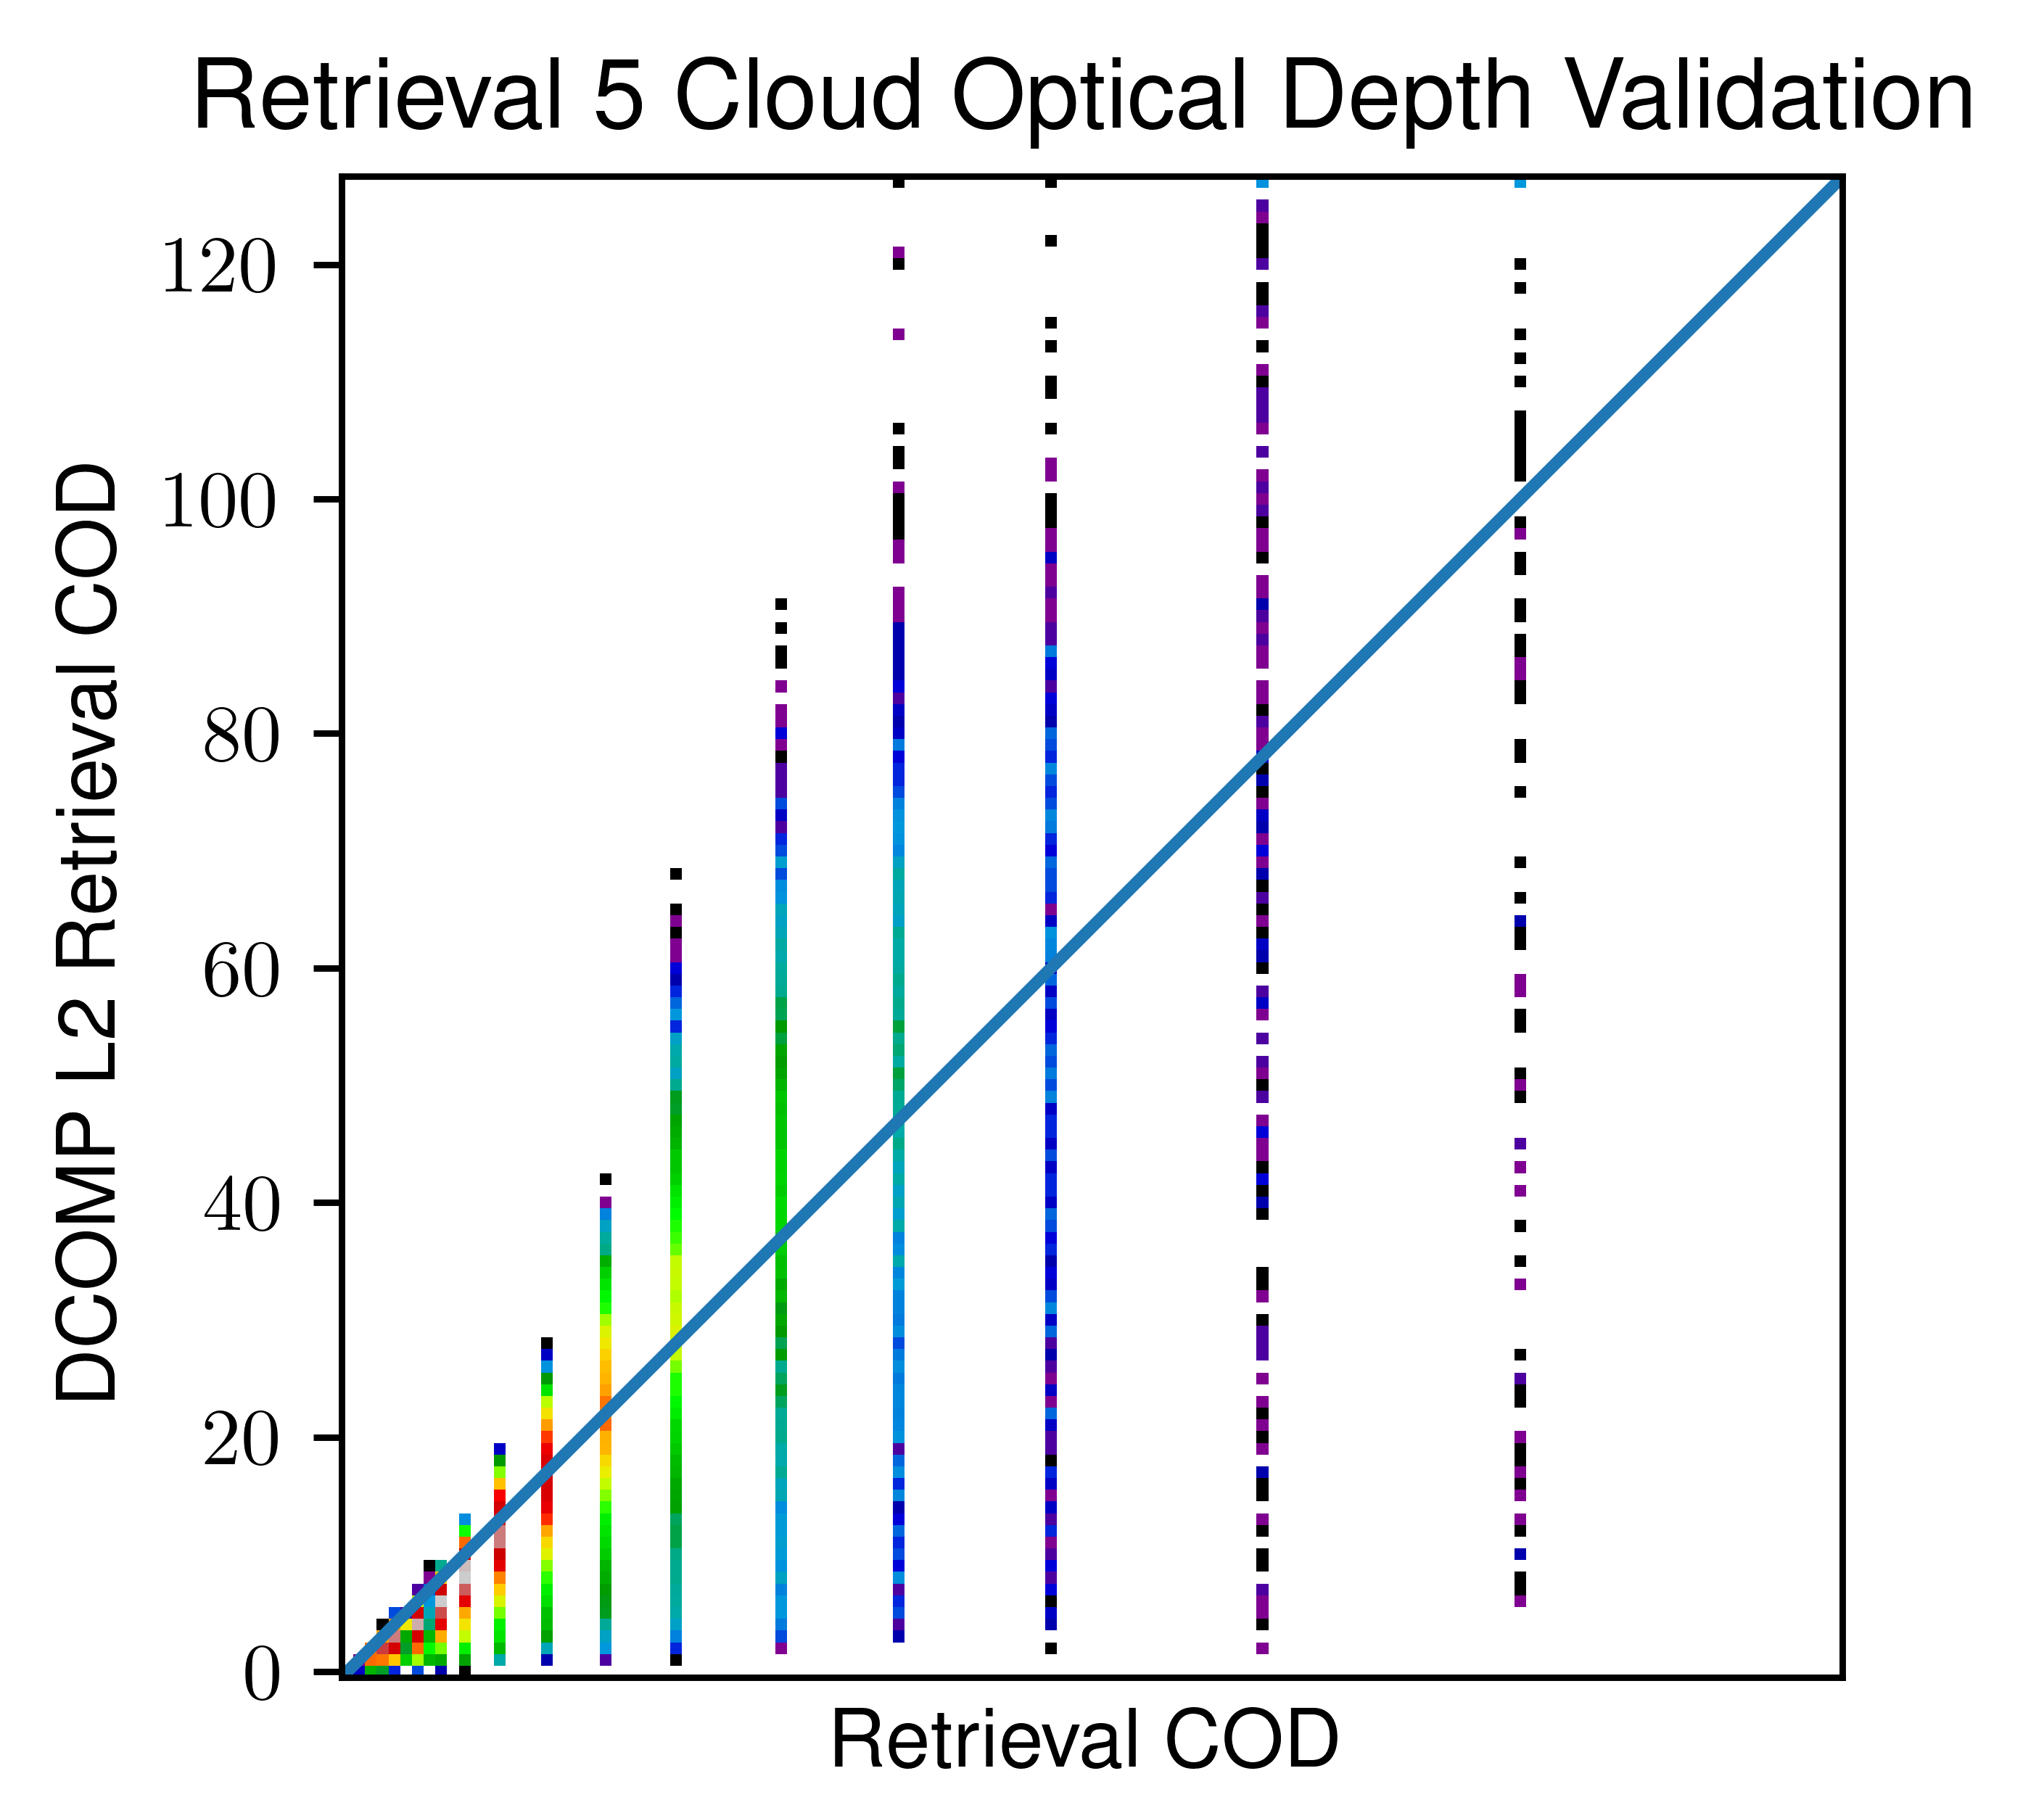
\includegraphics[width=.32\paperwidth]{figs/val_ret5_cod.png}
            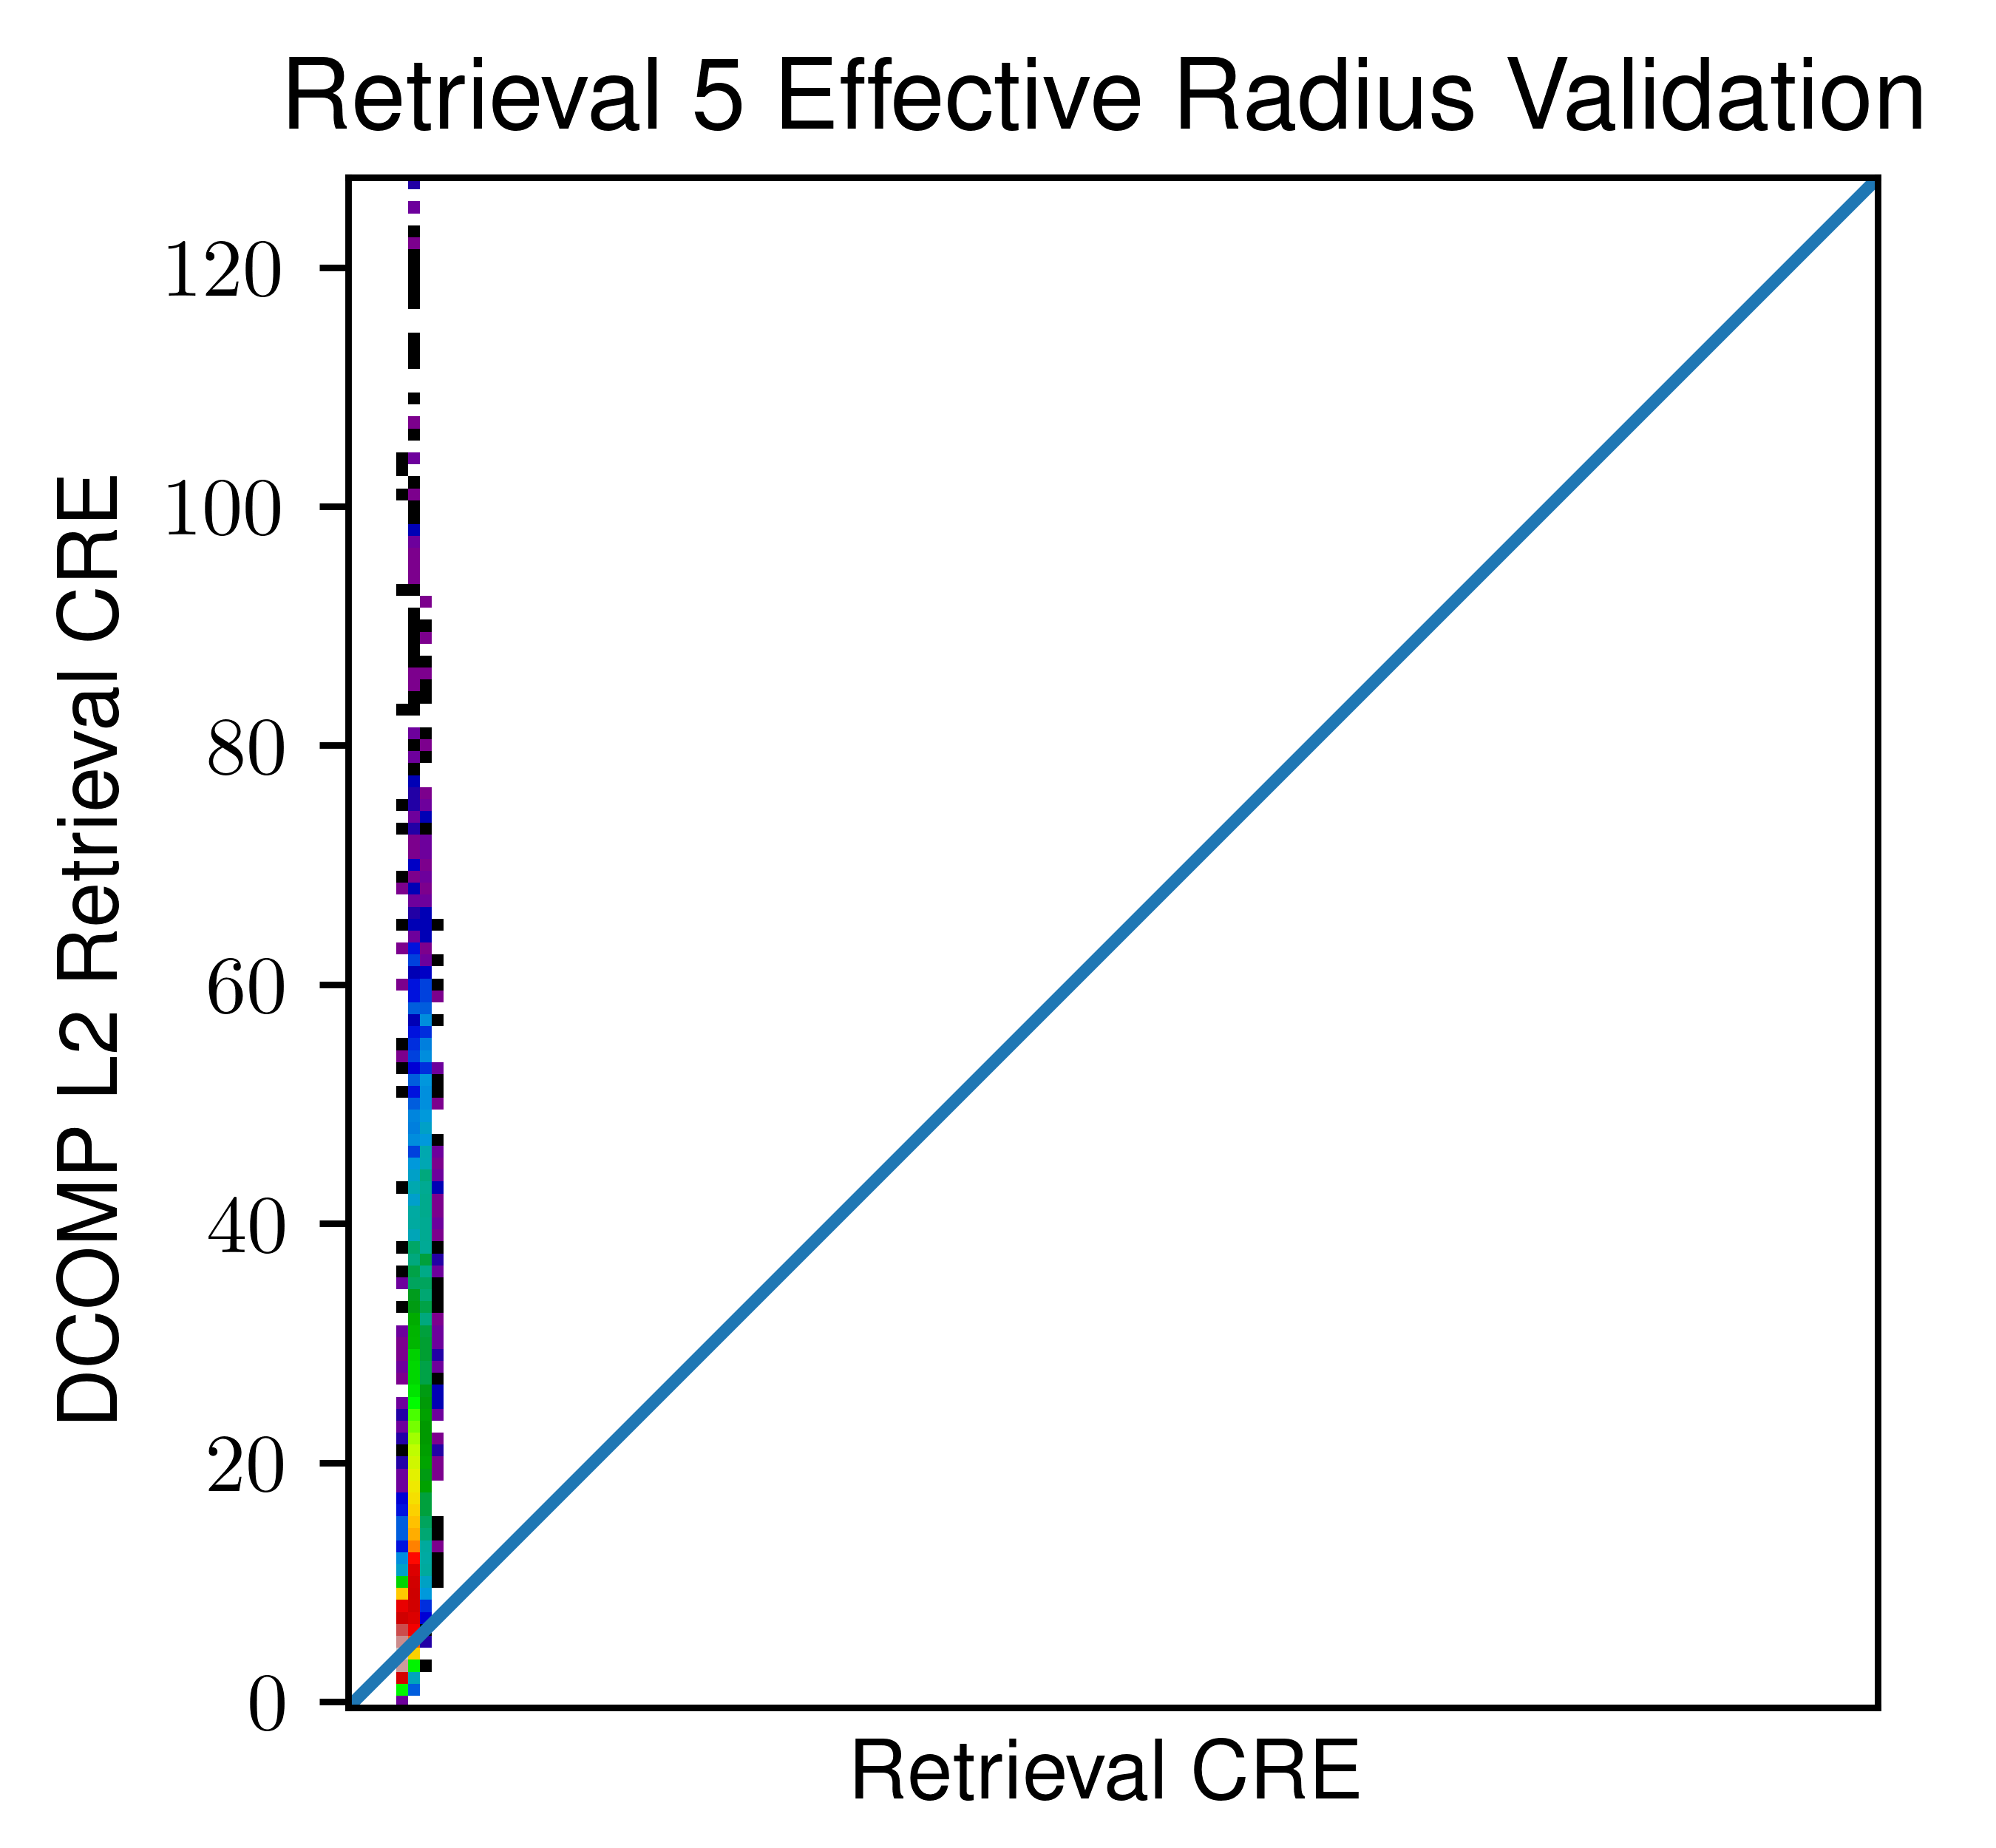
\includegraphics[width=.30\paperwidth]{figs/val_ret5_cre.png}
        }
        \makebox[\textwidth]{
            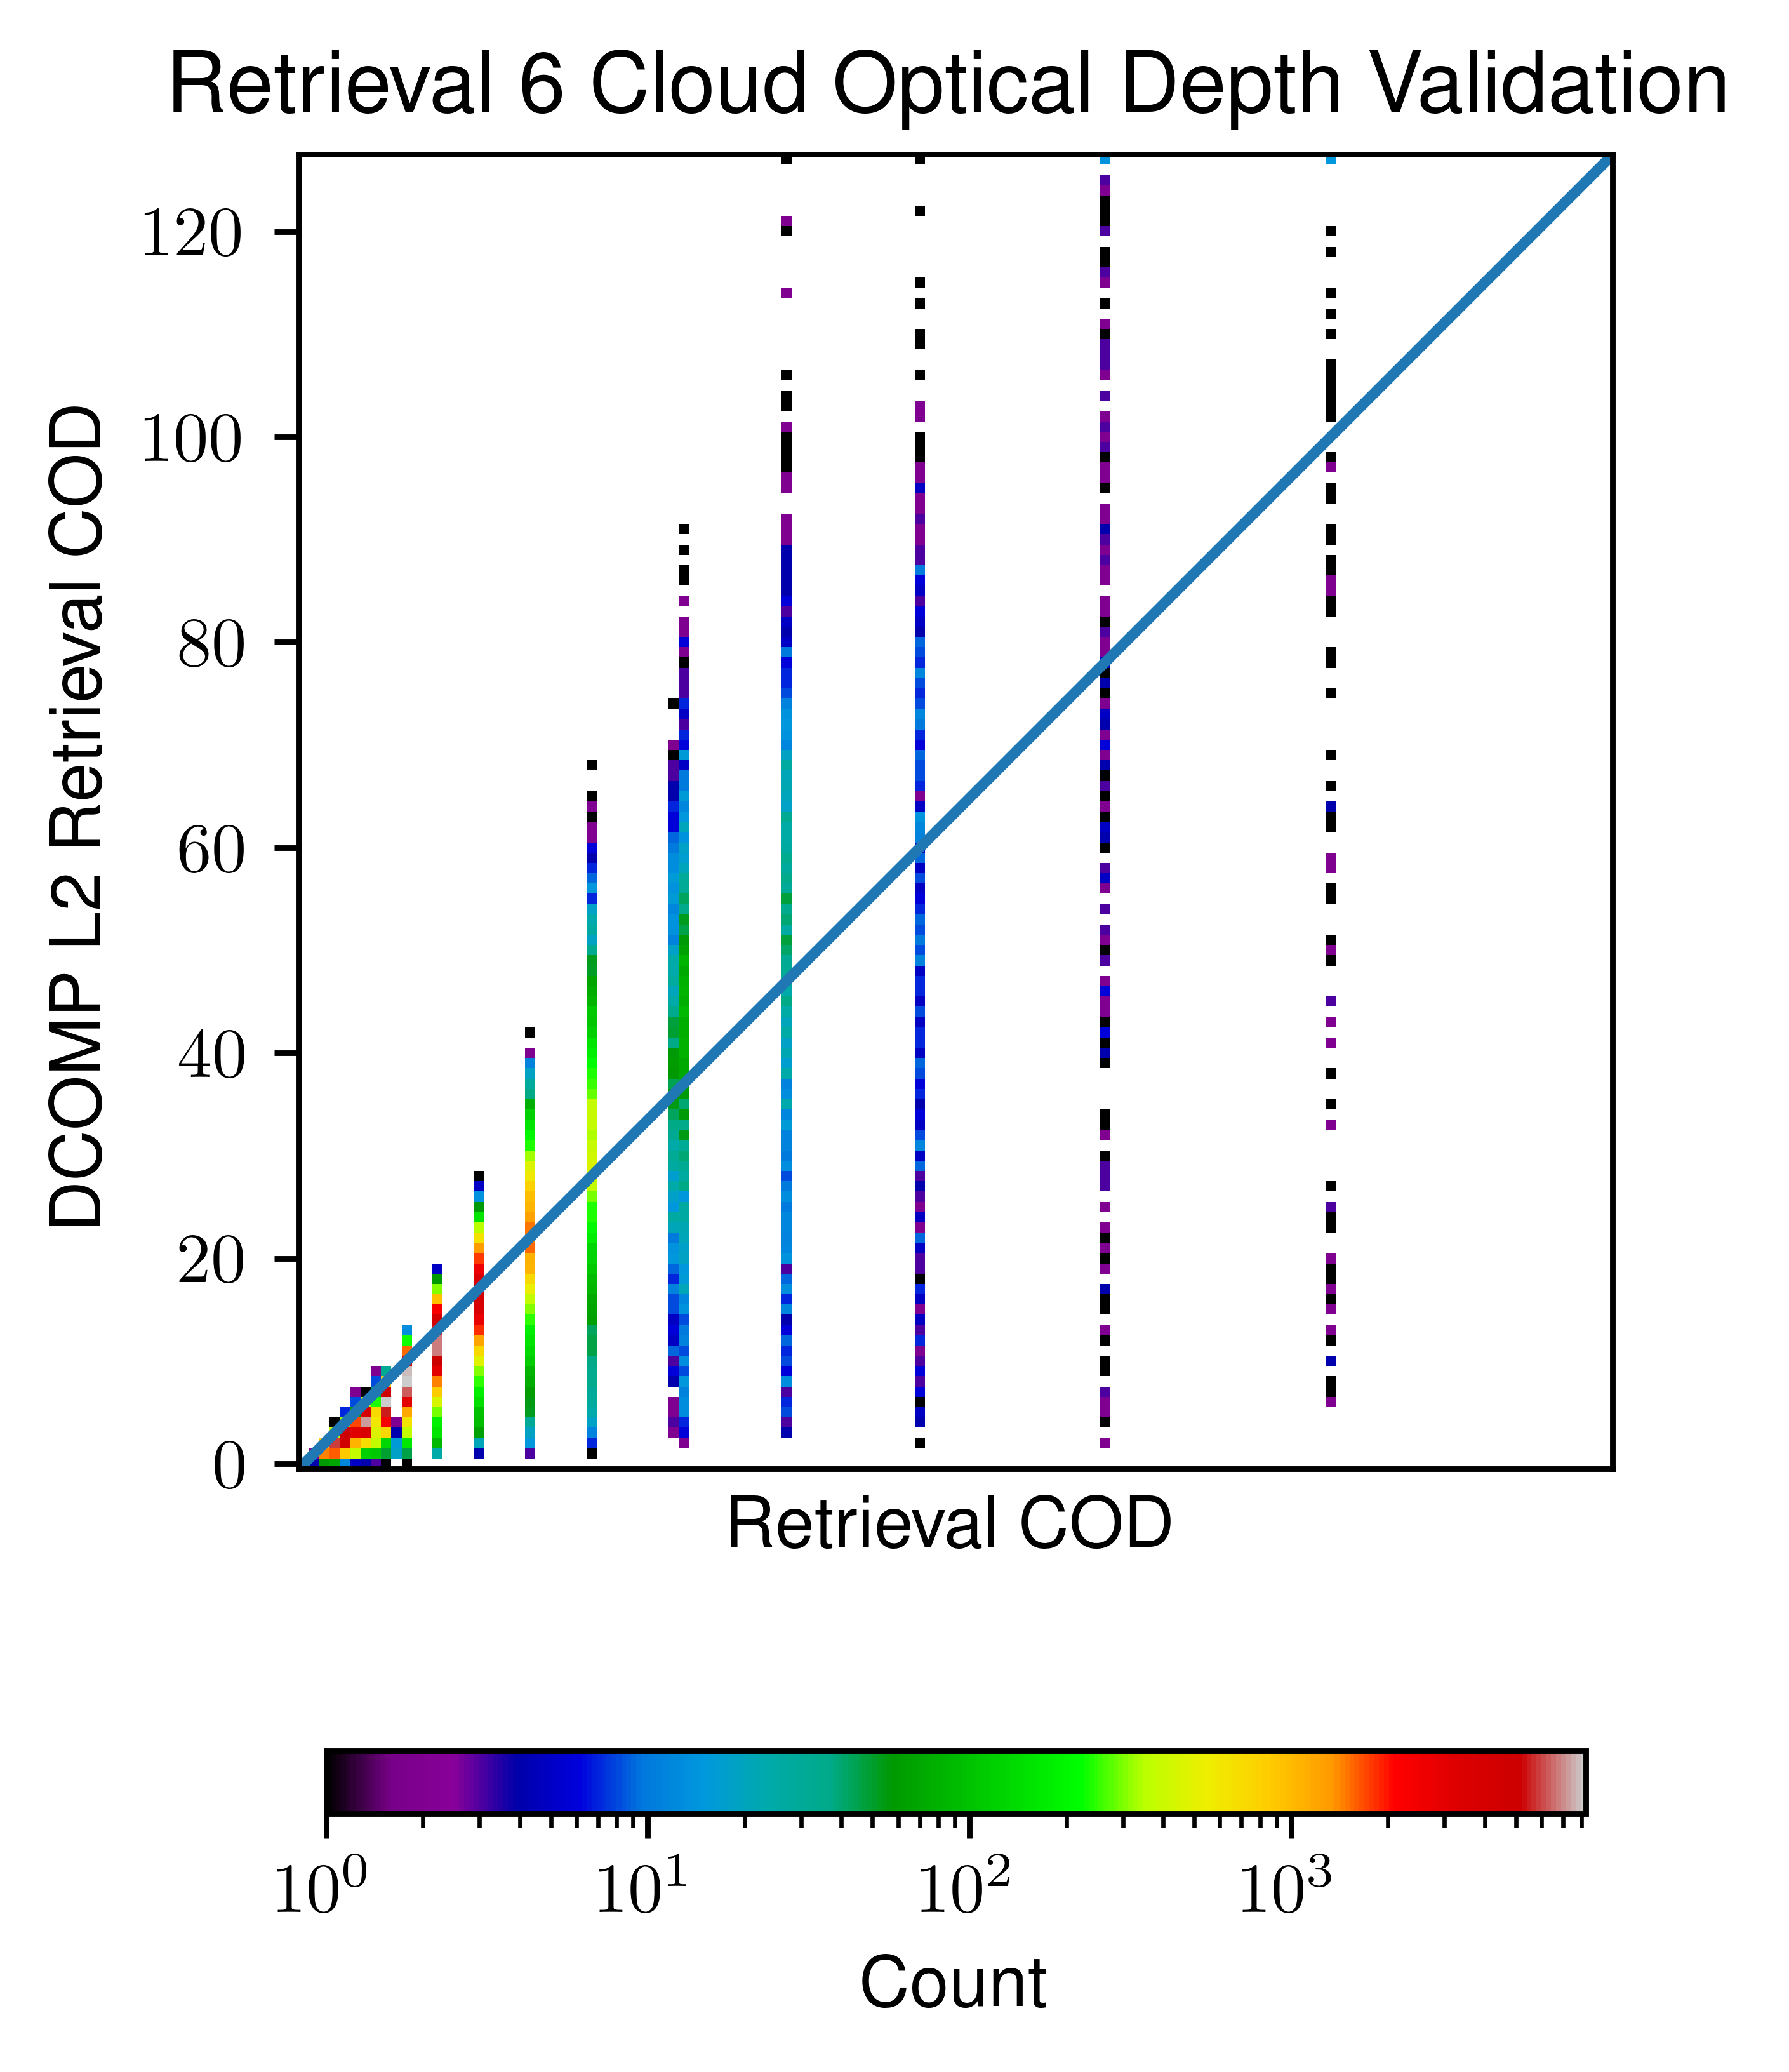
\includegraphics[width=.32\paperwidth]{figs/val_ret6_cod.png}
            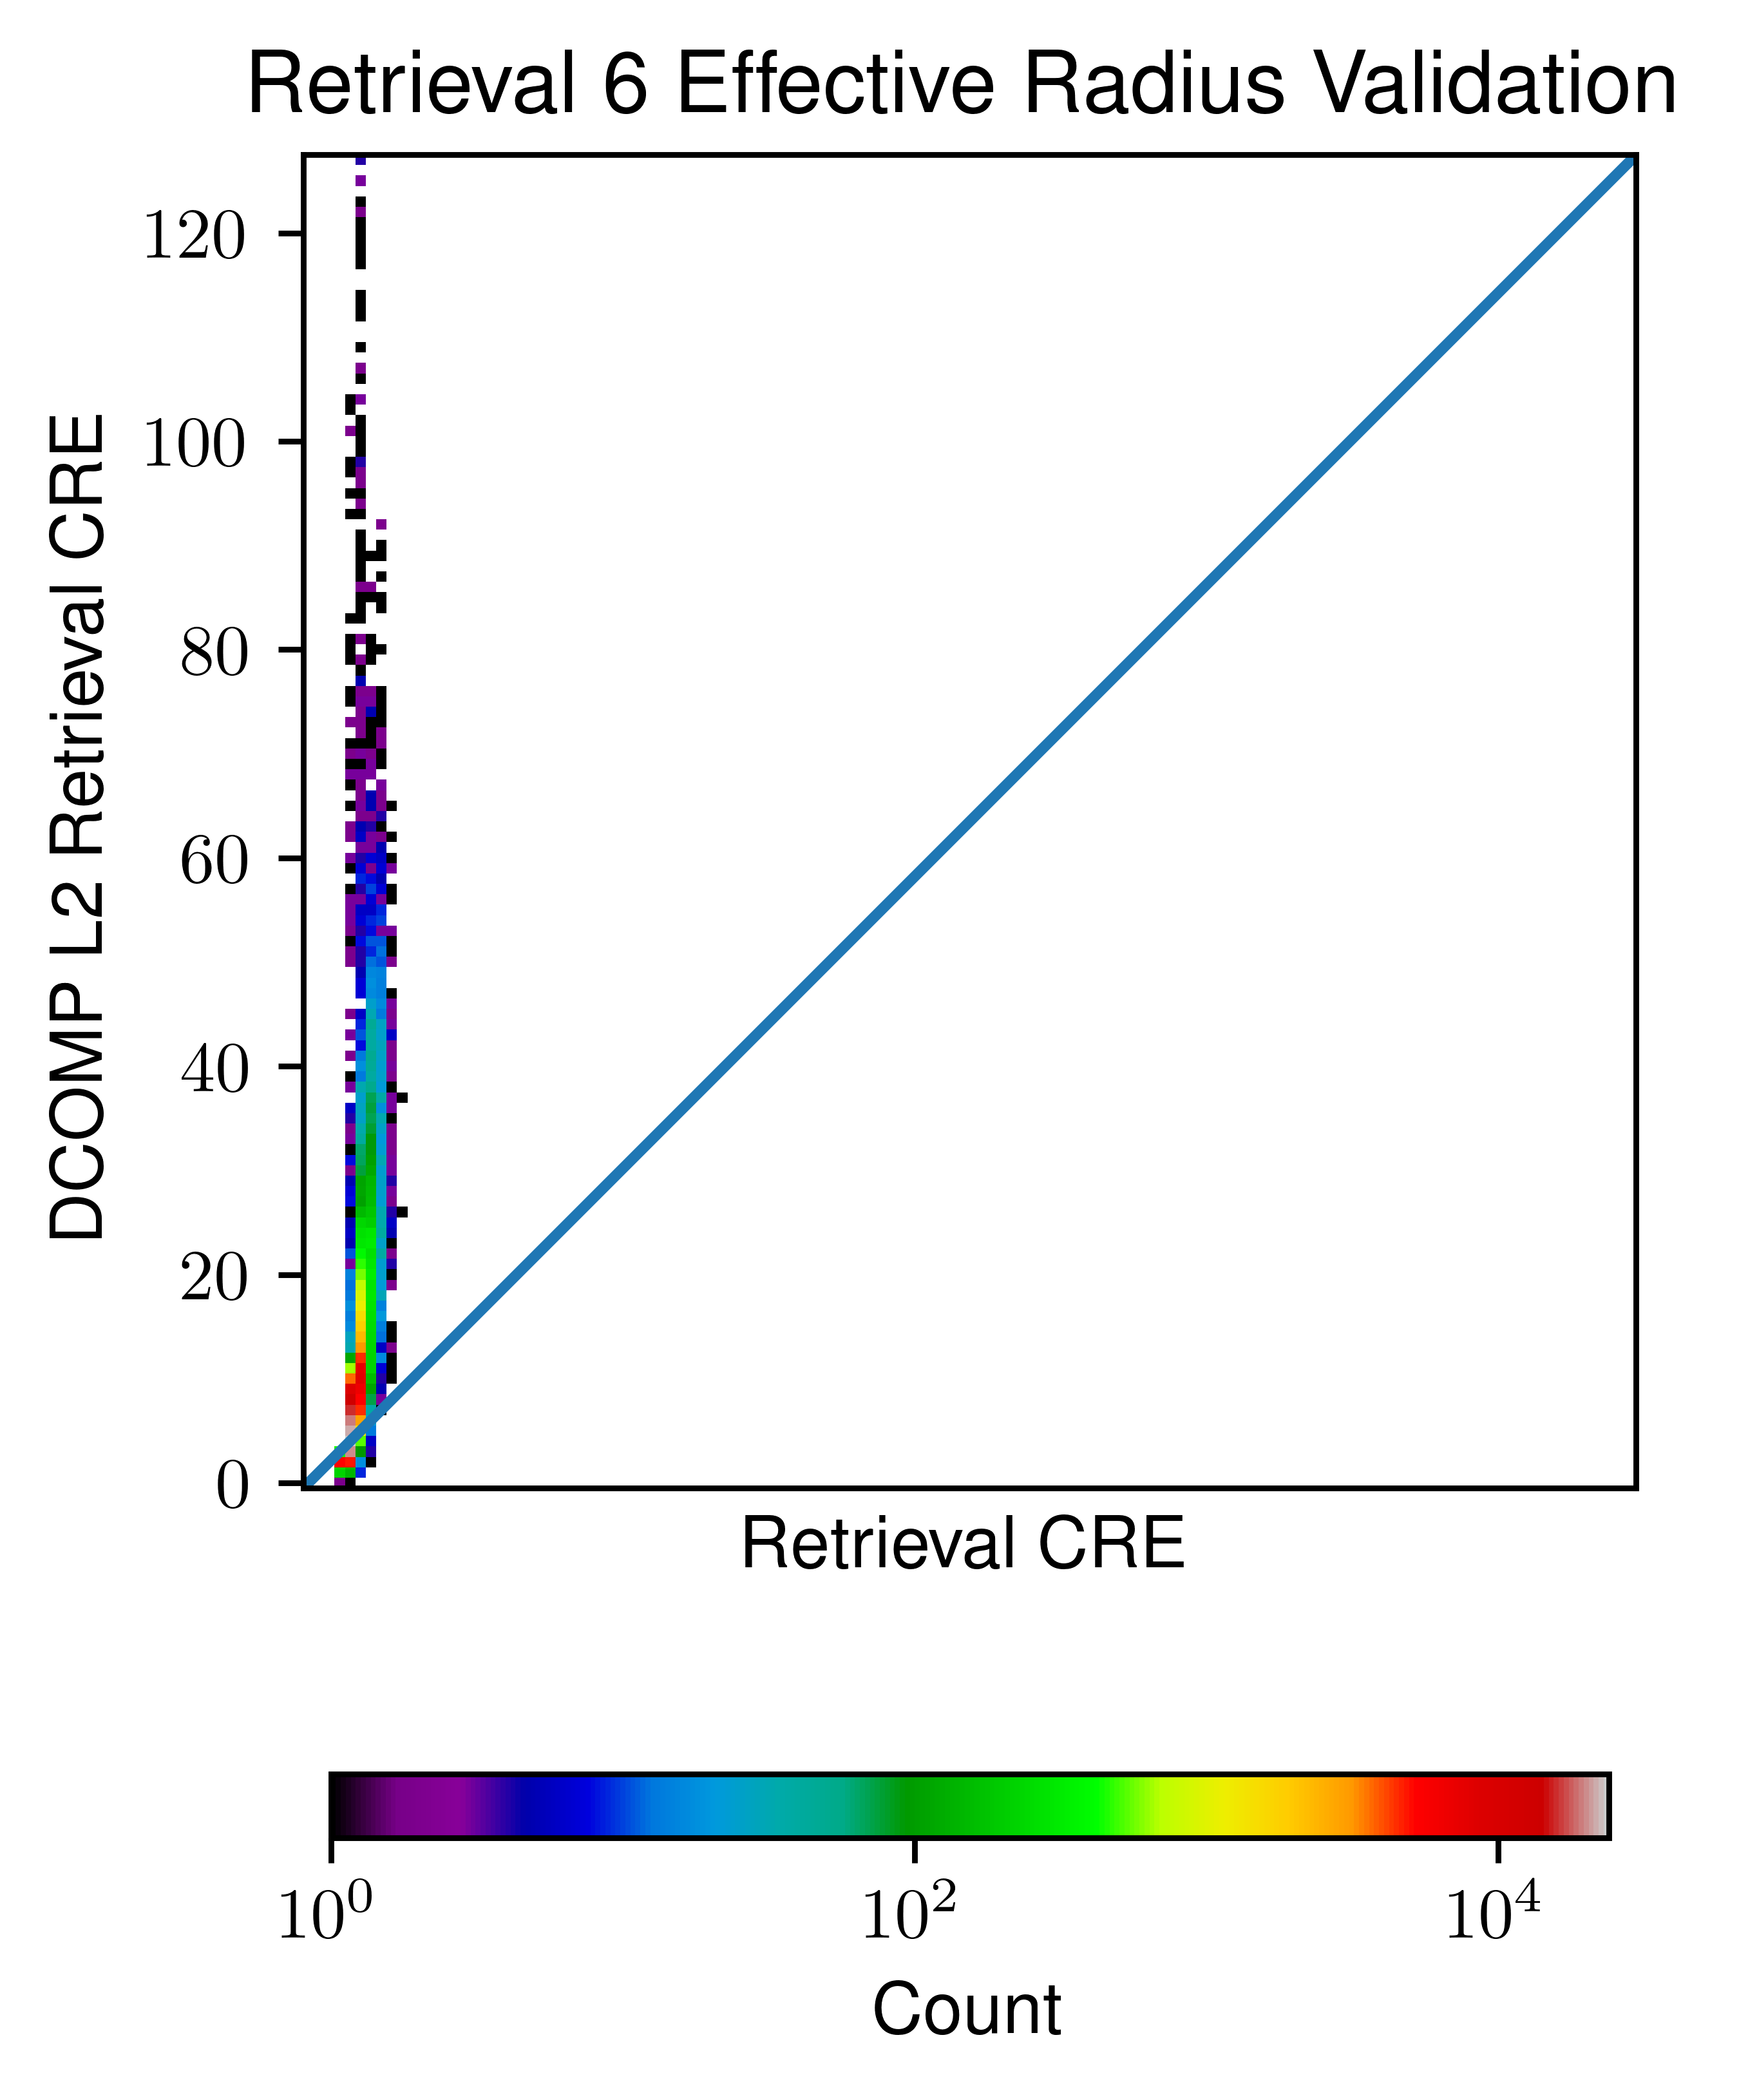
\includegraphics[width=.30\paperwidth]{figs/val_ret6_cre.png}
        }
    \end{center}
    \caption{A sample of failed retrievals, validated pixelwise against actual DCOMP L2 product values for the same image and domain. Retrieval 3 (top) follows DCOMP as closely as possible using the same error covariance matrices, cost function, and stopping conditions. Retrieval 5 (middle) doubles the a-priori and observation error covariance, doubles the maximum number of allowable iterations to 40, and stops on the first iteration with increasing cost. Finally, retrieval 6 (bottom) uses the identity matrix as the a-priori error covariance matrix, and also stops when cost increases.}
    \label{bad_retrievals}
\end{figure}

\clearpage

It's worth noting that DCOMP uses 45 lookup table bins for each of the geometric variables (solar zenith, viewing zenith, and relative azimuth),  while my lookup tables only include 21, 21, and 12 bins for the respective angles. In contrast, DCOMP only defines 9 effective radii and 29 optical depth bins, while I define 40 bins for each cloud property. Additionally, DCOMP performs a 5-dimensional interpolation of lookup table values (including geometry and cloud properties) using Newton's method, while I adopt the closest angle values for each pixel in a snap-to-grid fashion, and only interpolate the cloud property state vector. This discrepancy is certainly a source of error in my process, however the simplification frees up a substantial amount of compute, and I doubt that it plays a major role in the issue of moving away from the a-priori values.

\subsection{Role of A-Priori Error Covariance}

After several attempts, and upon close inspection of Figure \ref{bad_retrievals}, I realized that $\tau_c$ and $r_e$ values were able to start moving further away from their initial guesses when I set the a-priori error covariance matrix $S_a$ to progressively higher values. I decided to set the diagonal elements of the matrix to the excessively high value of 100, and obtained the results in Figures \ref{big_sa_val} and \ref{big_sa_err}.

\begin{figure}[h!]
    \centering
    \begin{center}
        \makebox[\textwidth]{
            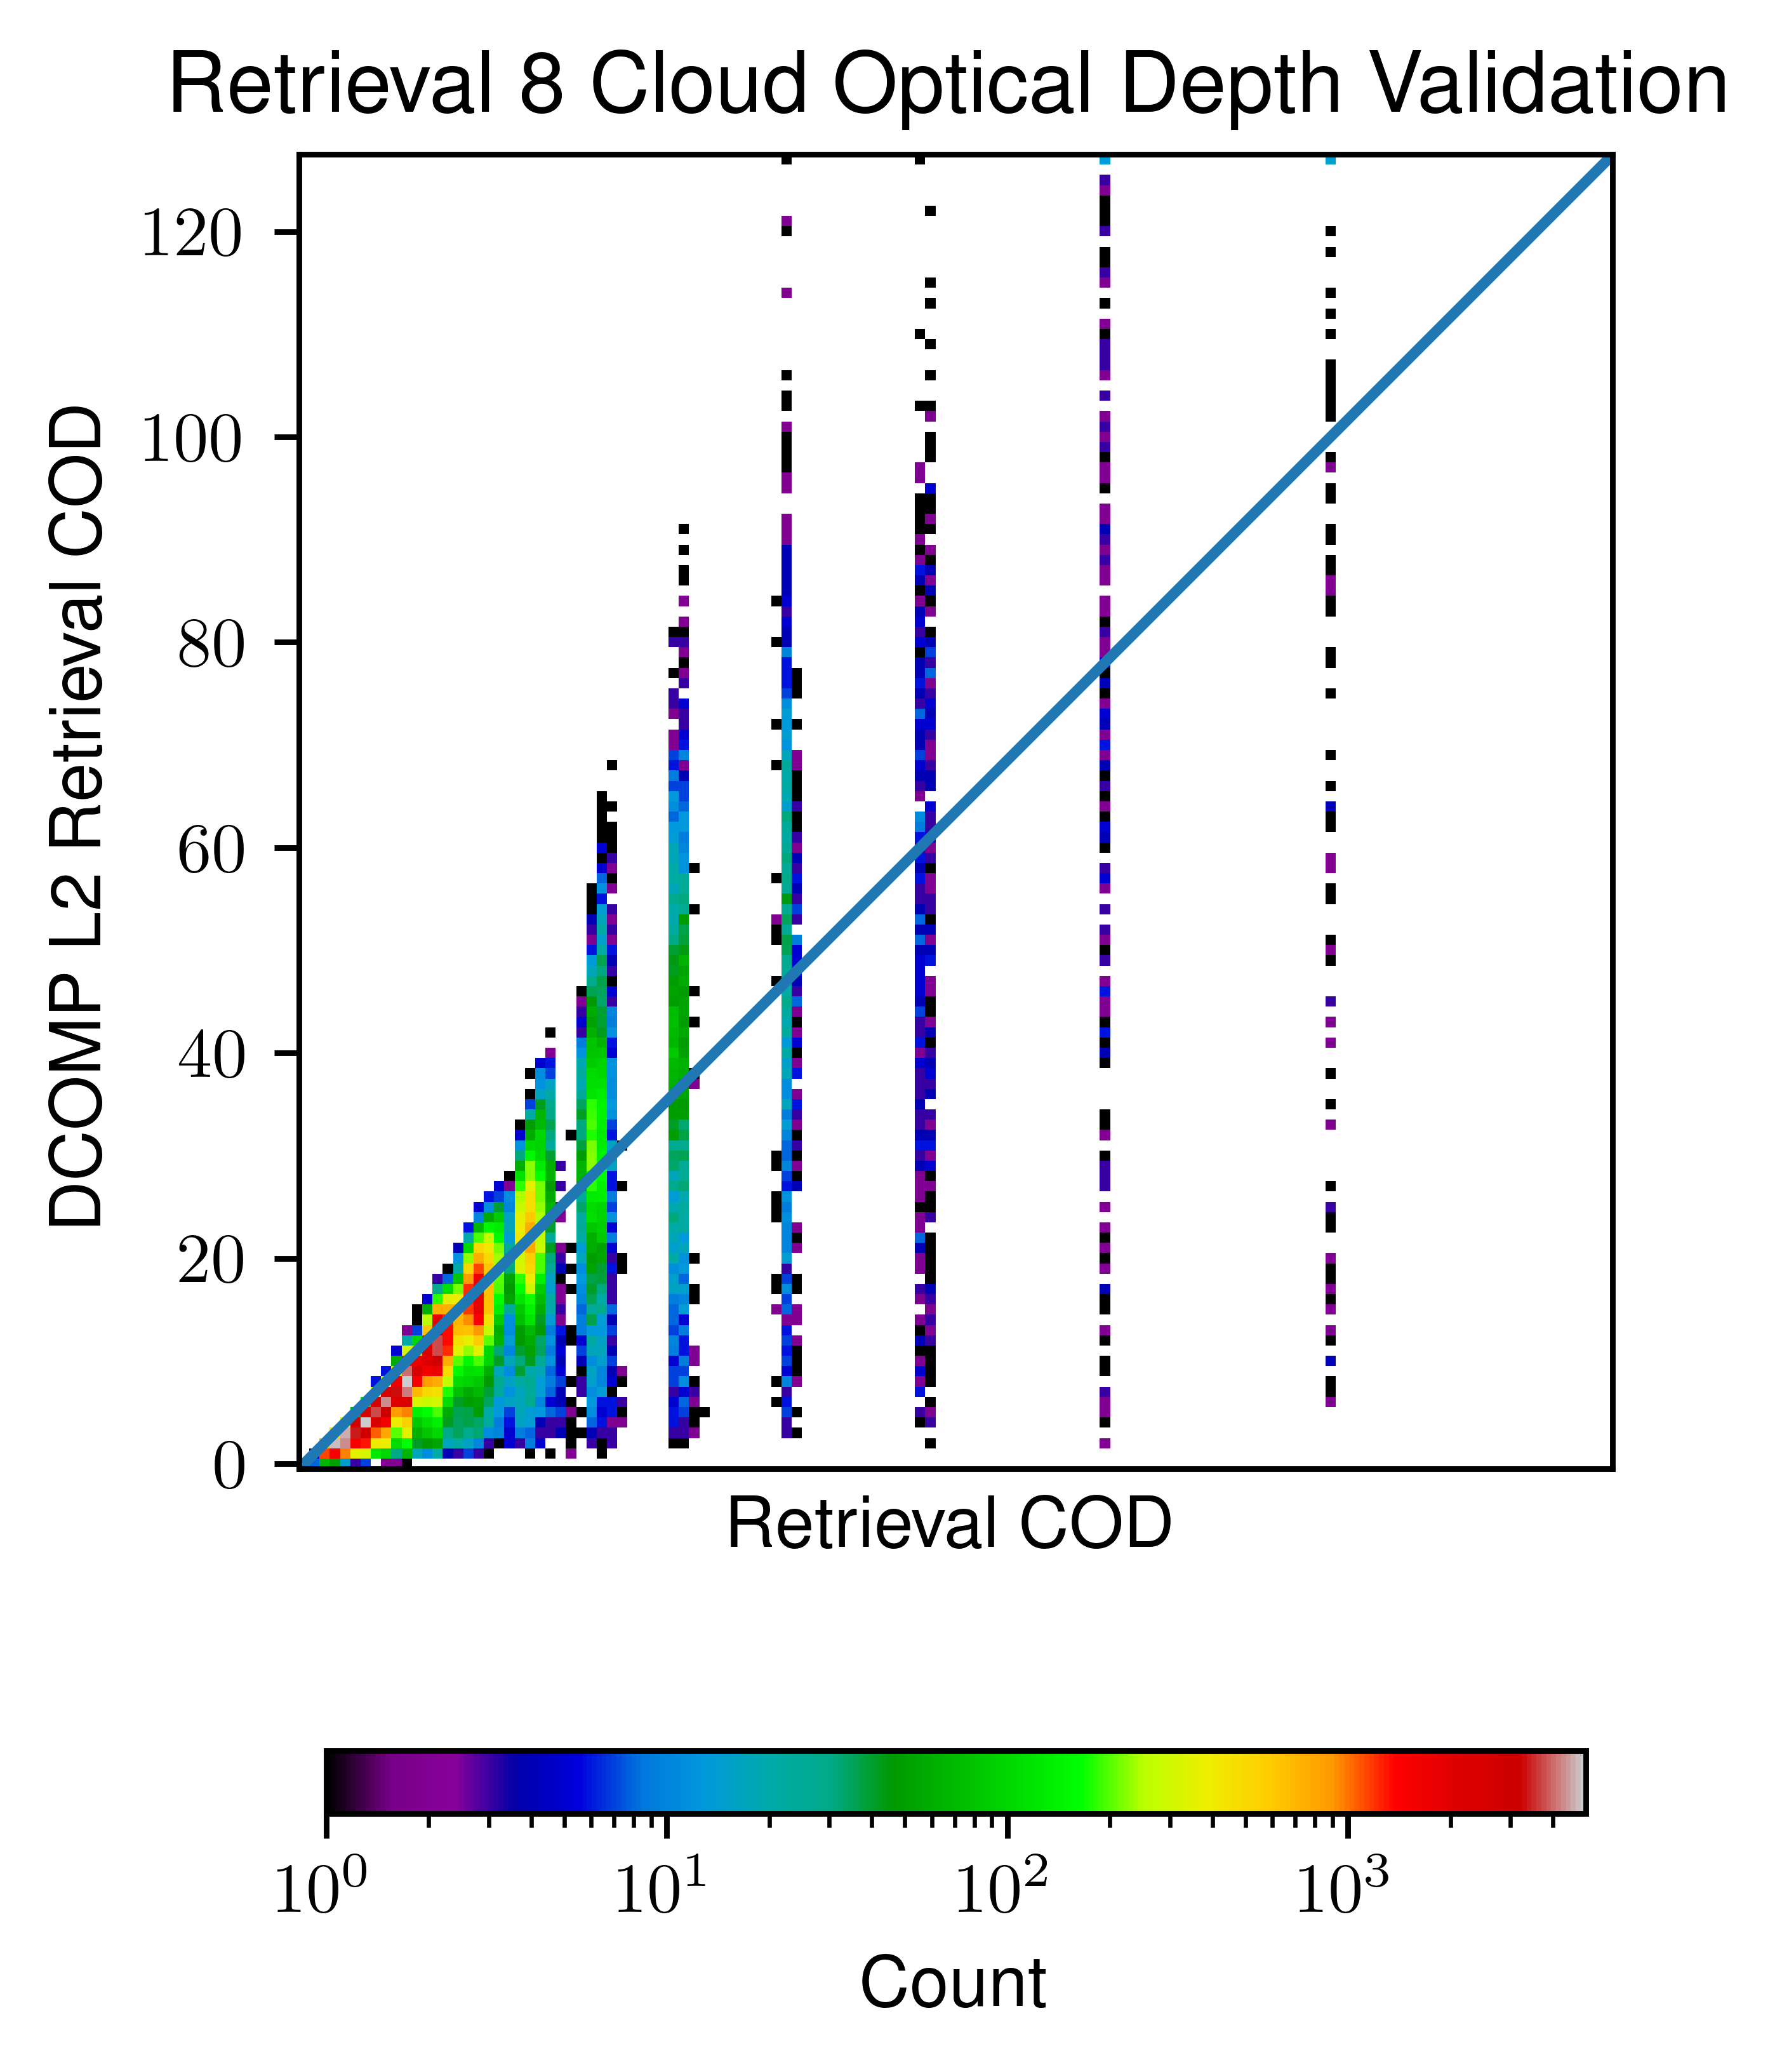
\includegraphics[width=.35\paperwidth]{figs/val_ret8_cod.png}
            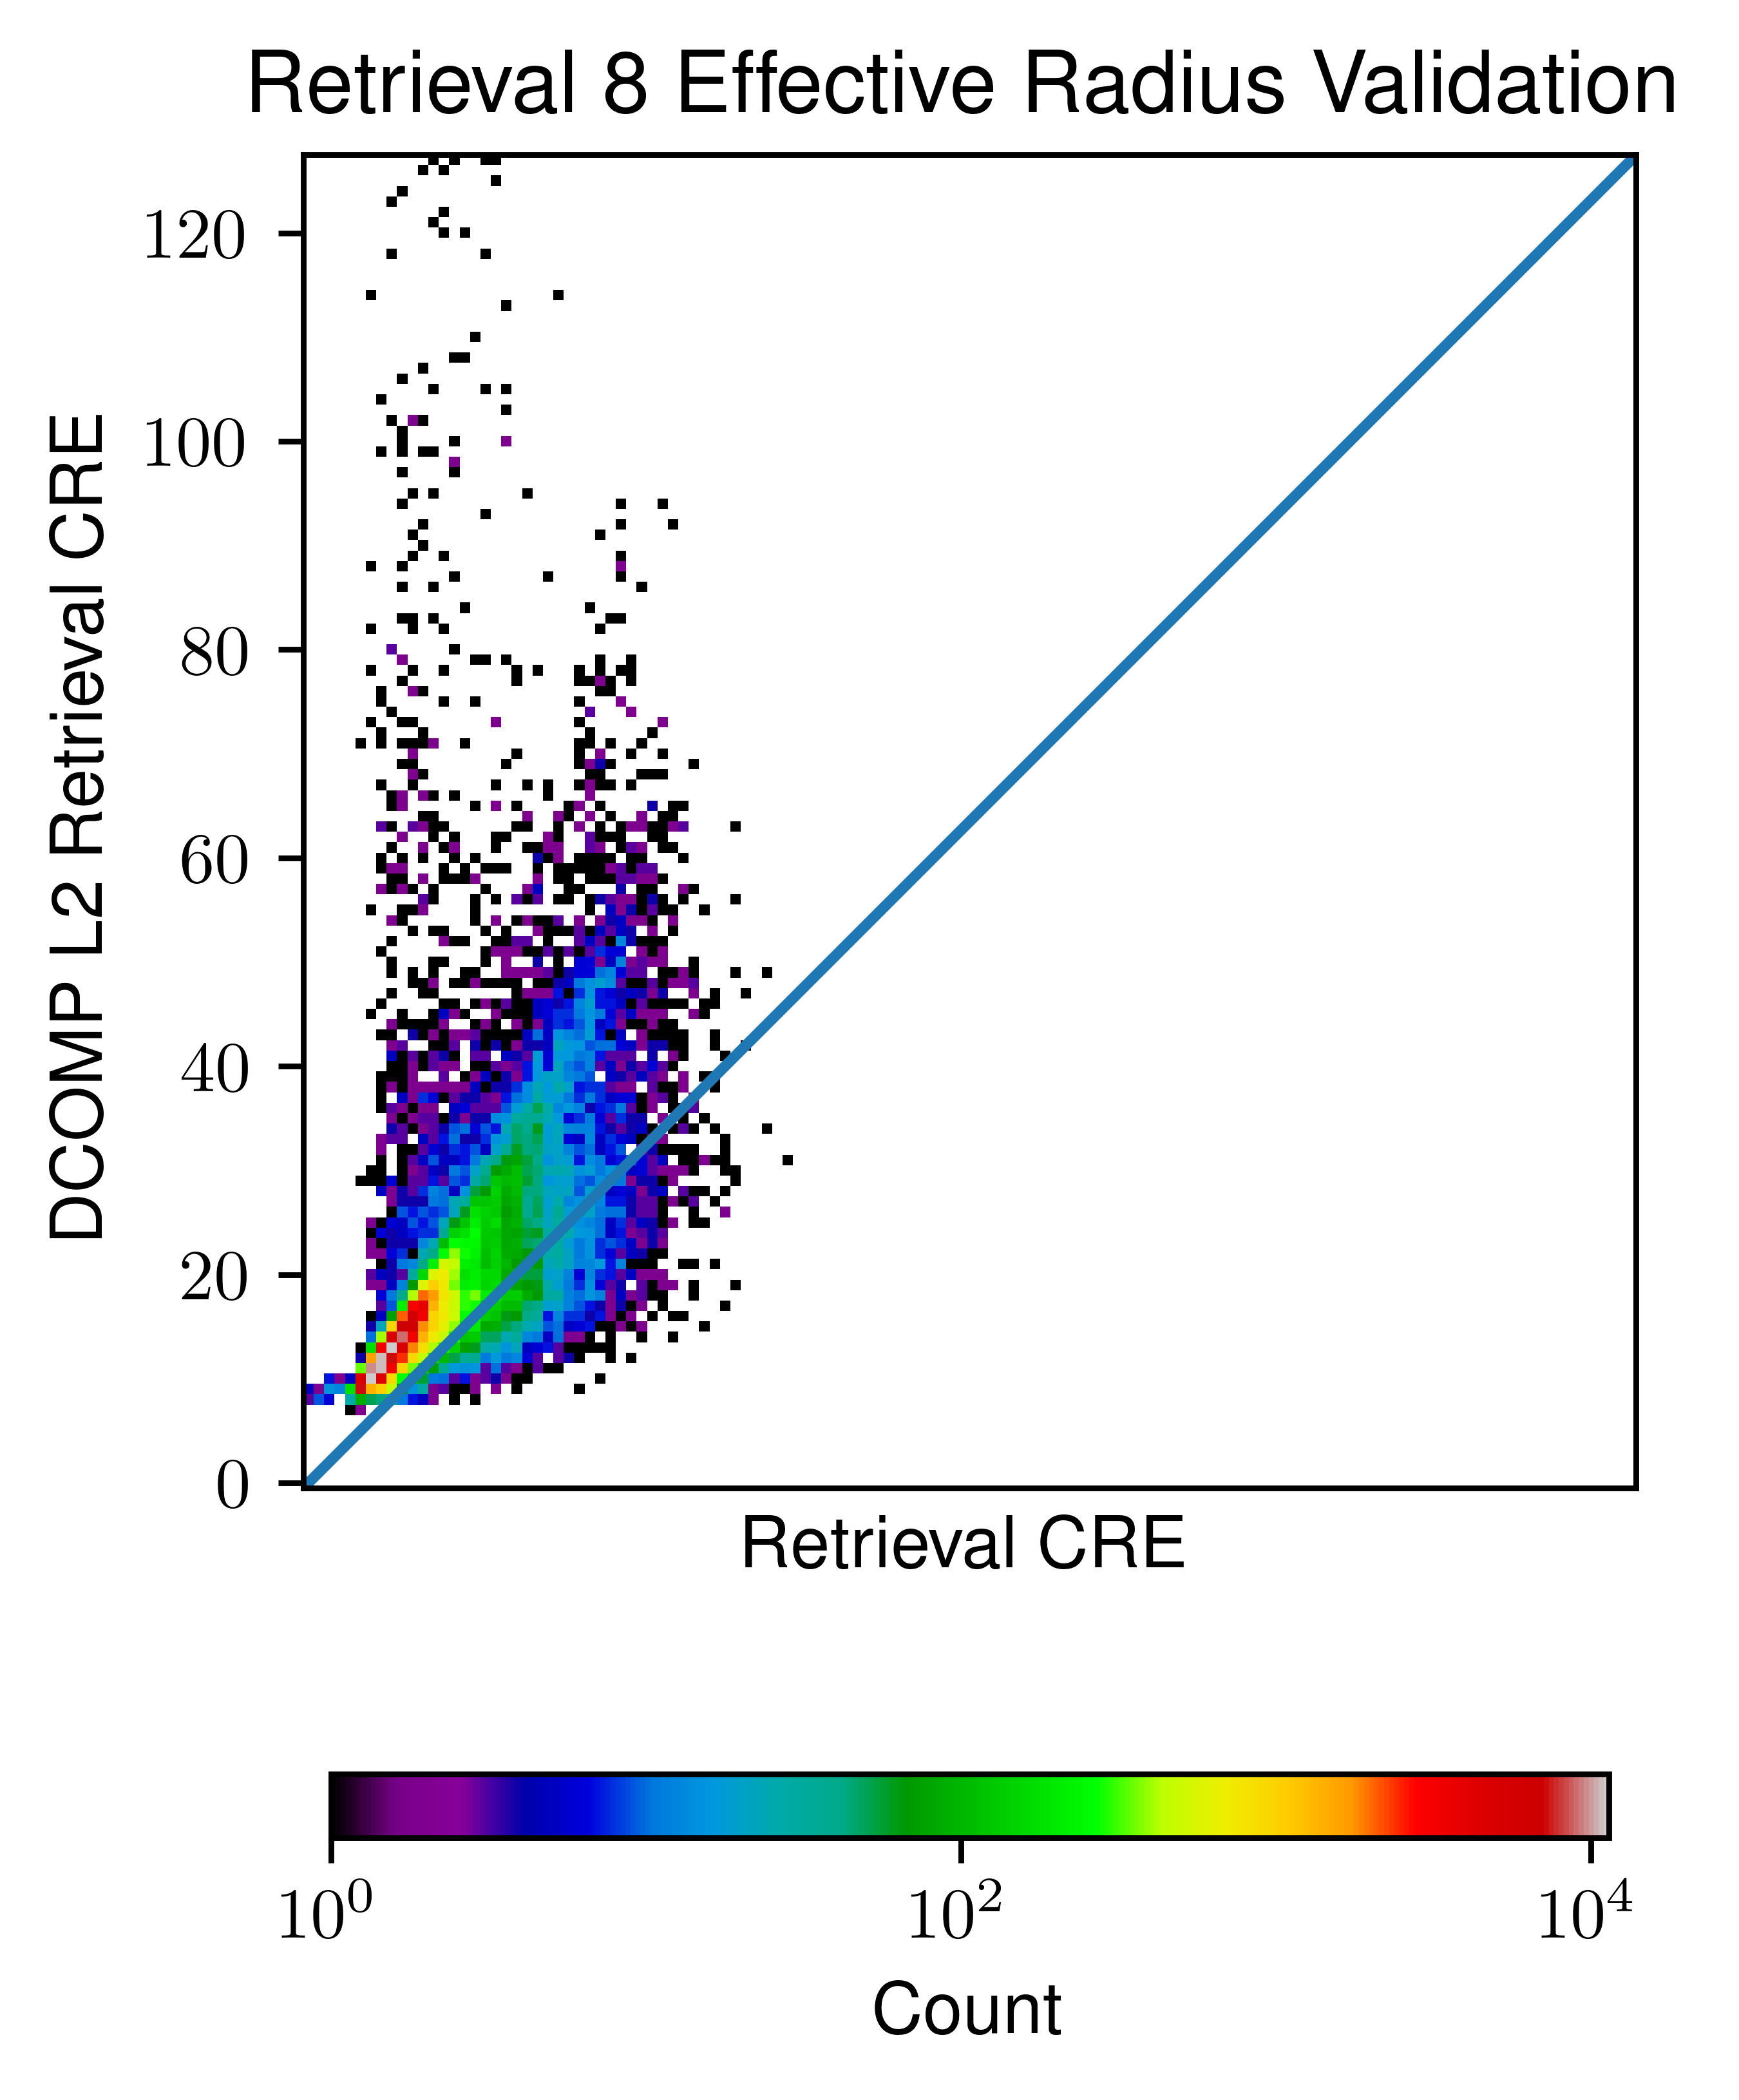
\includegraphics[width=.32\paperwidth]{figs/val_ret8_cre.png}
        }
    \end{center}
    \caption{Validation curves for the retrieval with very large $S_a$ values. Although COD values at the extremes of optical thickness are still too discrete, which suggests they haven't moved away from their initial values, the optical depths of clouds with typical values are well-characterized. Effective radius measurements are biased towards underestimate, but have finally started to move away from the $10\mu m$ baseline.}
    \label{big_sa_val}
\end{figure}

\begin{figure}[h!]
    \centering
    \begin{center}
        \makebox[\textwidth]{
            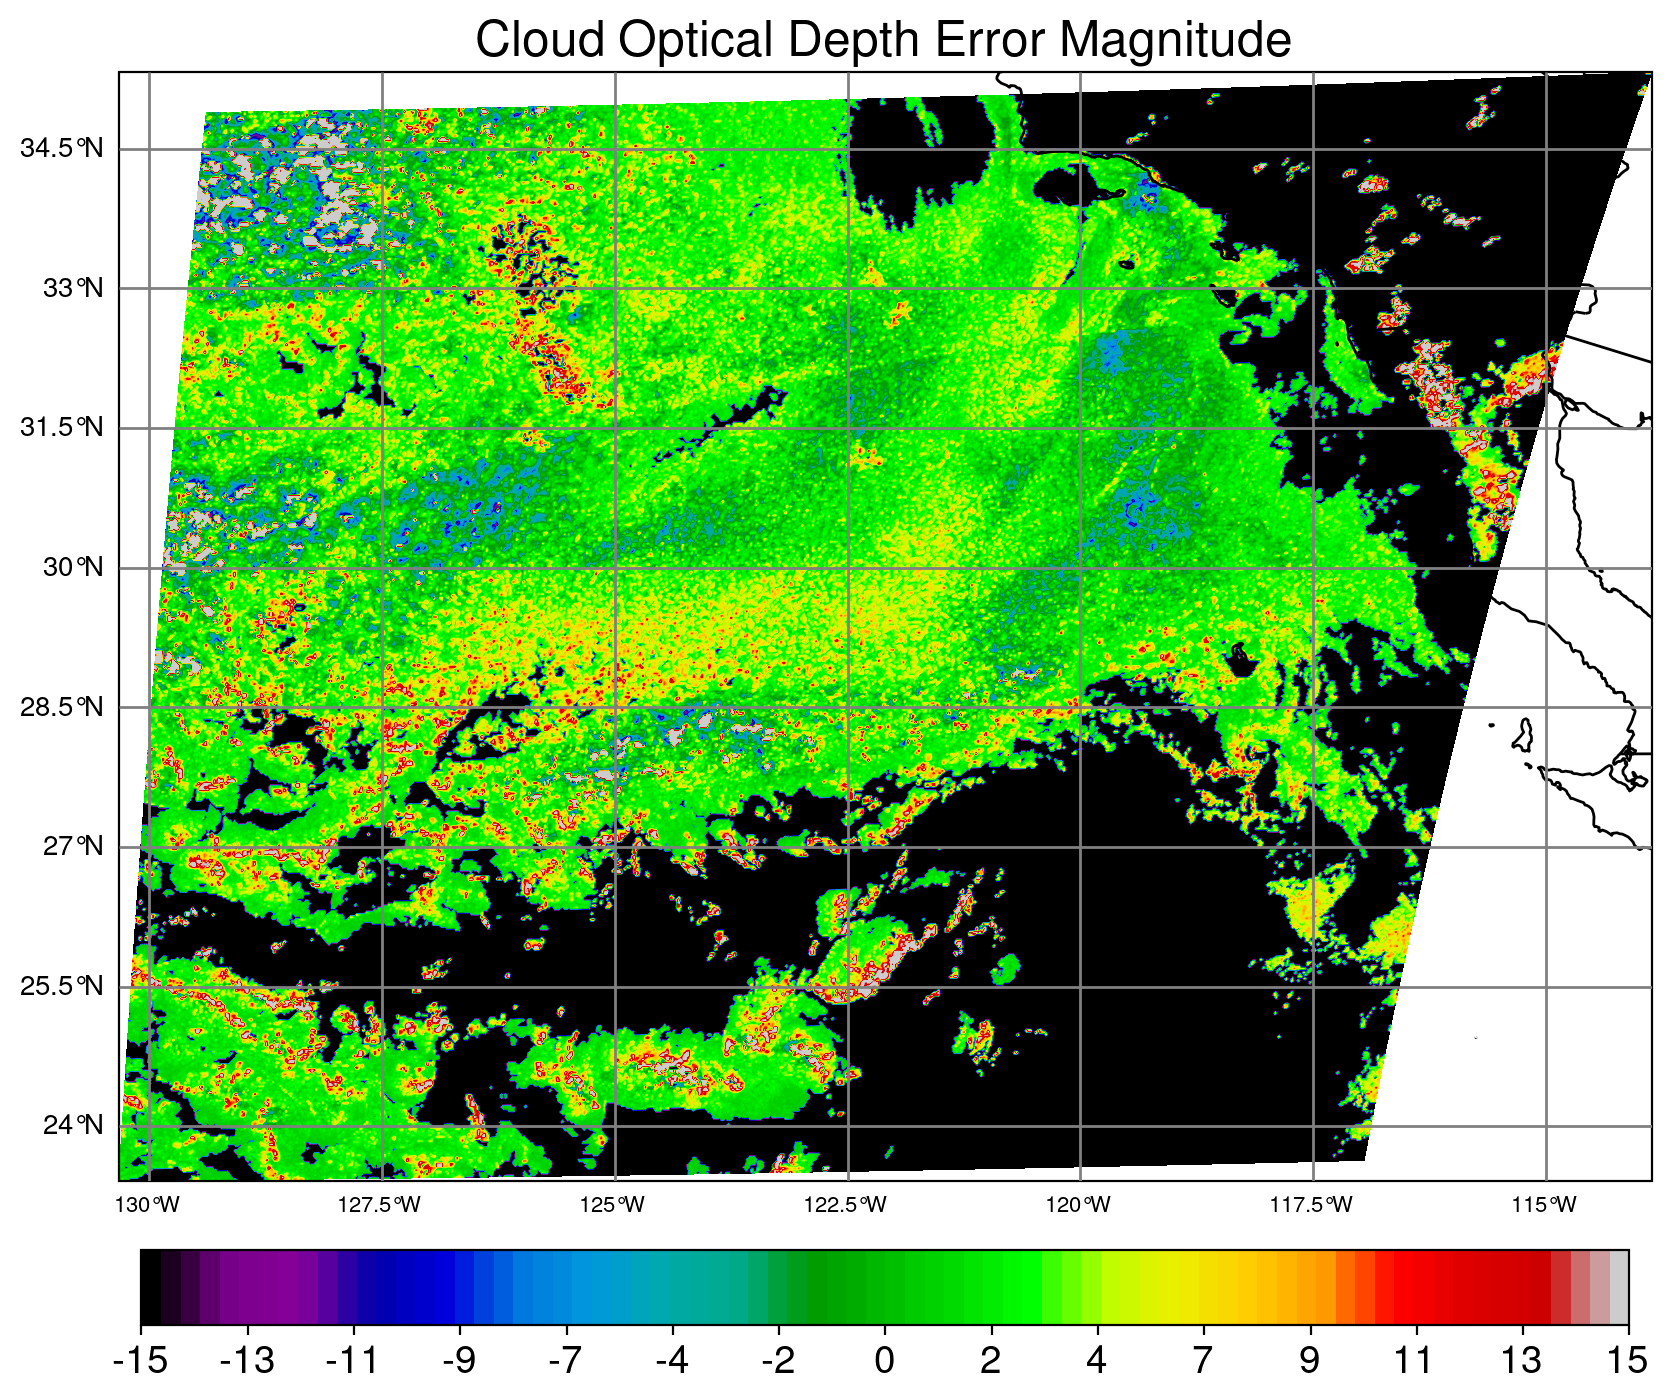
\includegraphics[width=.35\paperwidth]{figs/ret8_cod-err.png}
            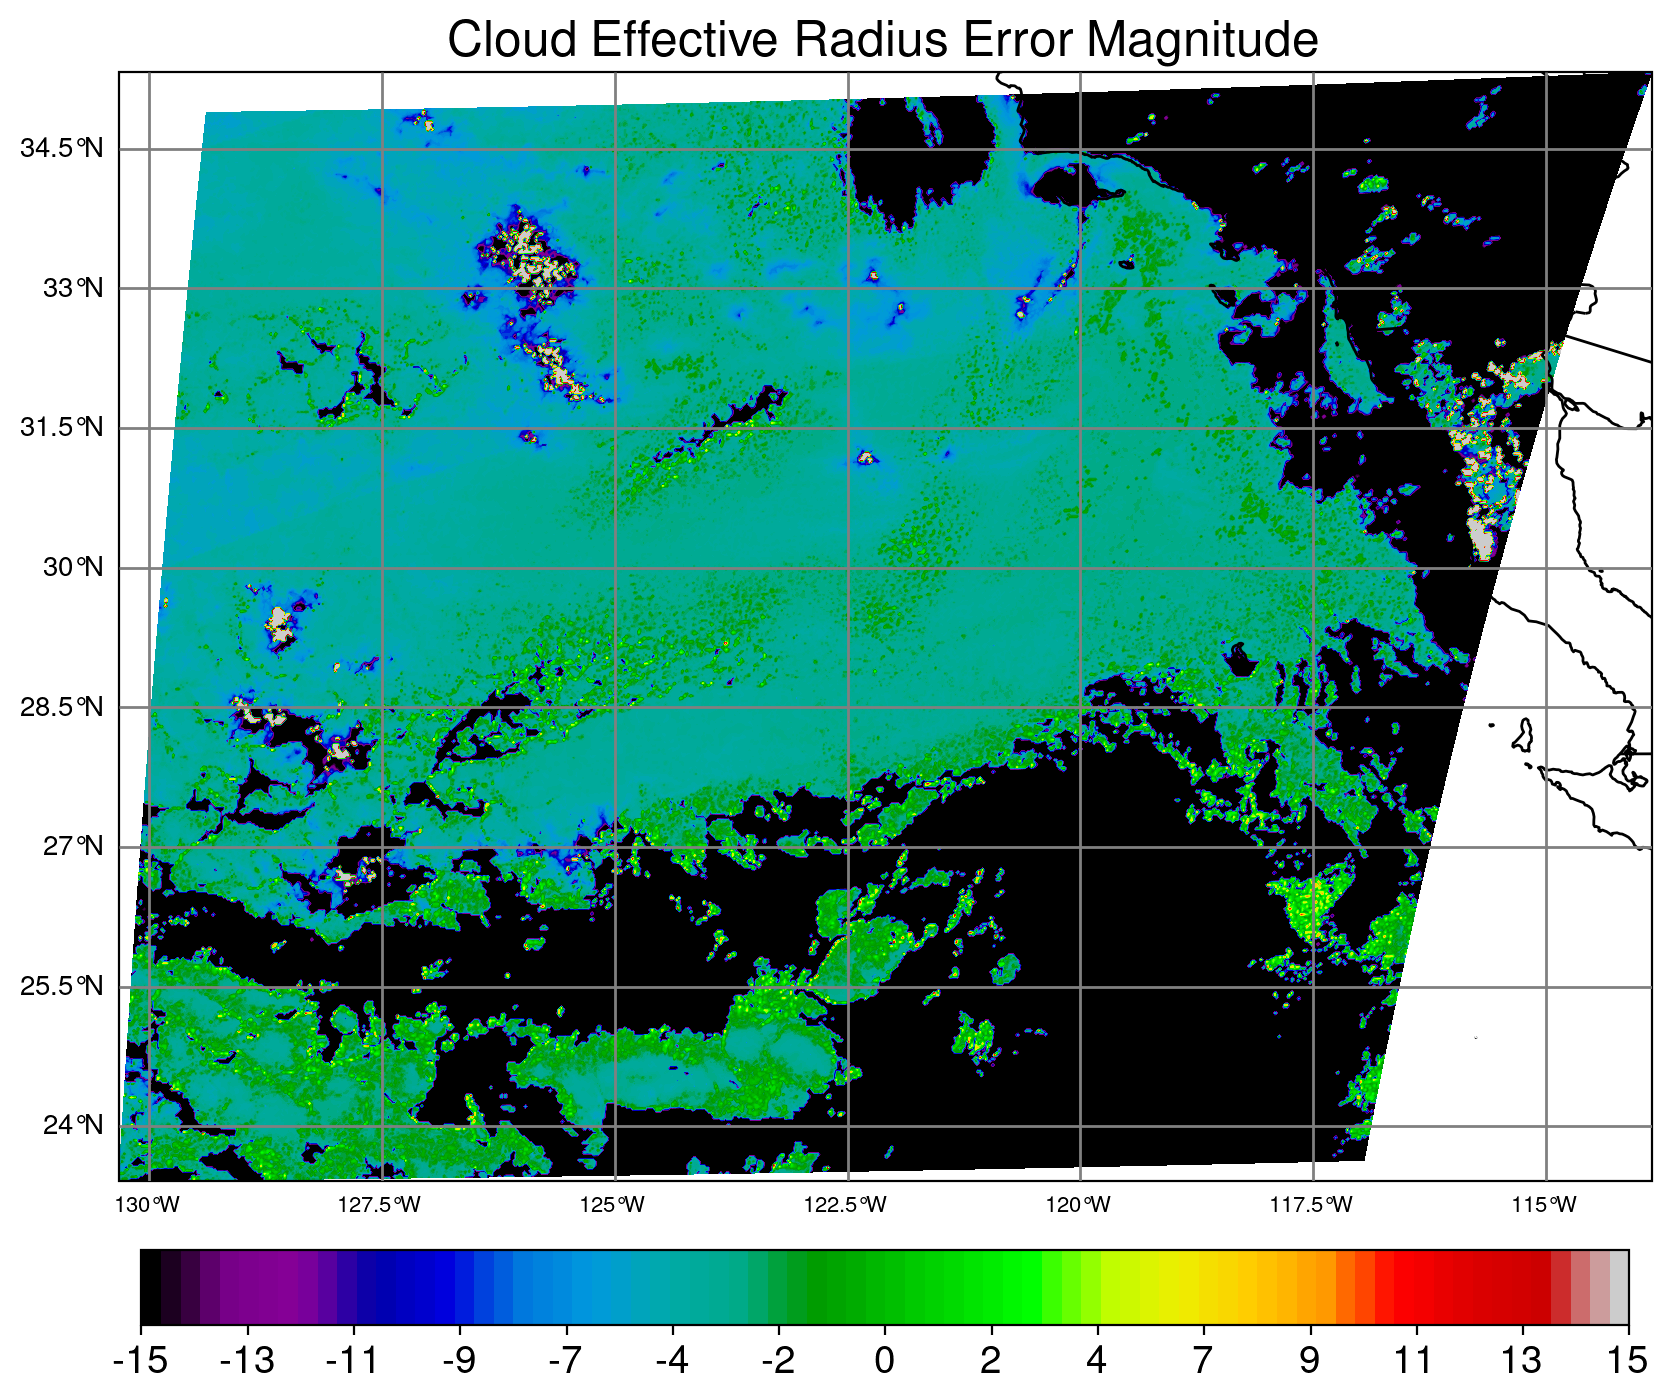
\includegraphics[width=.35\paperwidth]{figs/ret8_cre-err.png}
        }
    \end{center}
    \caption{Error magnitude for the retrieval with large $S_a$ values. Notice that much of the error is contributed by the low-lying fog over California. This is reasonable since the surface albedo is likely much higher.}
    \label{big_sa_err}
\end{figure}

\vspace{-2em}

\subsection{Alternative Retrieval Method}

As a sanity check, I adopted a ``brute-force'' method of determining the state of each pixel by implementing the following procedure instead of iterating over the state vector; these steps are a drop-in replacement for steps $4-4.8$ in the retrieval algorithm process from Section \ref{dcomp_algo}. I would actually argue that brute-force here is a misnomer since, unlike the method outlined in DCOMP, this procedure doesn't involve any guess-and-checking. Furthermore, unlike the DCOMP which can only be efficiently parallelized if lookup tables are stored in read-only shared memory, this retrieval process is conducive to per-pixel multithreading with vectorized numpy array operations. As such, it generally takes less than a minute to run, which is a couple of orders of magnitude faster than running DCOMP on a single thread.  For each pixel identified as a cloud...

\begin{enumerate}
    \setlength\itemsep{-.2em}
    \item Reduce the lookup table to the geometric values that are closest to the pixel's values.
    \item Calculate the euclidean distance of reflectance in both channels between the observation and lookup table grid.
    \item Of the 2 closest reflectance values on the LUT grid, select the one that with a euclidean distance in $[\tau_c, r_e]$ space which is closest to the a-priori value.
    \item Calculate the offset in the observed reflectance in both channels from the lower-bound surrounding grid point.
    \item Determine the partial change in $\tau_c$ with respect to the VIS reflectance and $r_e$ with respect to the NIR reflectance surrounding the selected point.
    \item Using the partial changes and offsets, return an estimate for the $[\tau_c, r_e]$ pixel state.
\end{enumerate}

To be fair, the advantage of this new method would be diminished if I had attempted to parallelize the original procedure, and the computational complexity of new method increases exponentially with each additional lookup table dimension. Additionally, the reliance on euclidean distance for choosing grid point candidates is a major weakness in the absence of data normalization since the charactaristic scales of reflectance are different between the VIS and NIR channels, and the scale of COD differs from that of CRE. A further shortcoming of the new method is that by only calculating partial derivatives of each property with respect to one channel, it relies more heavily on the assumption that $\tau_c$ and $r_e$ are independent of each other. If my cloud property lookup table points weren't very fine (compared to the DCOMP ATBD), this would probably be a significant source of error.

\begin{figure}[h!]
    \centering
    \begin{center}
        \makebox[\textwidth]{
            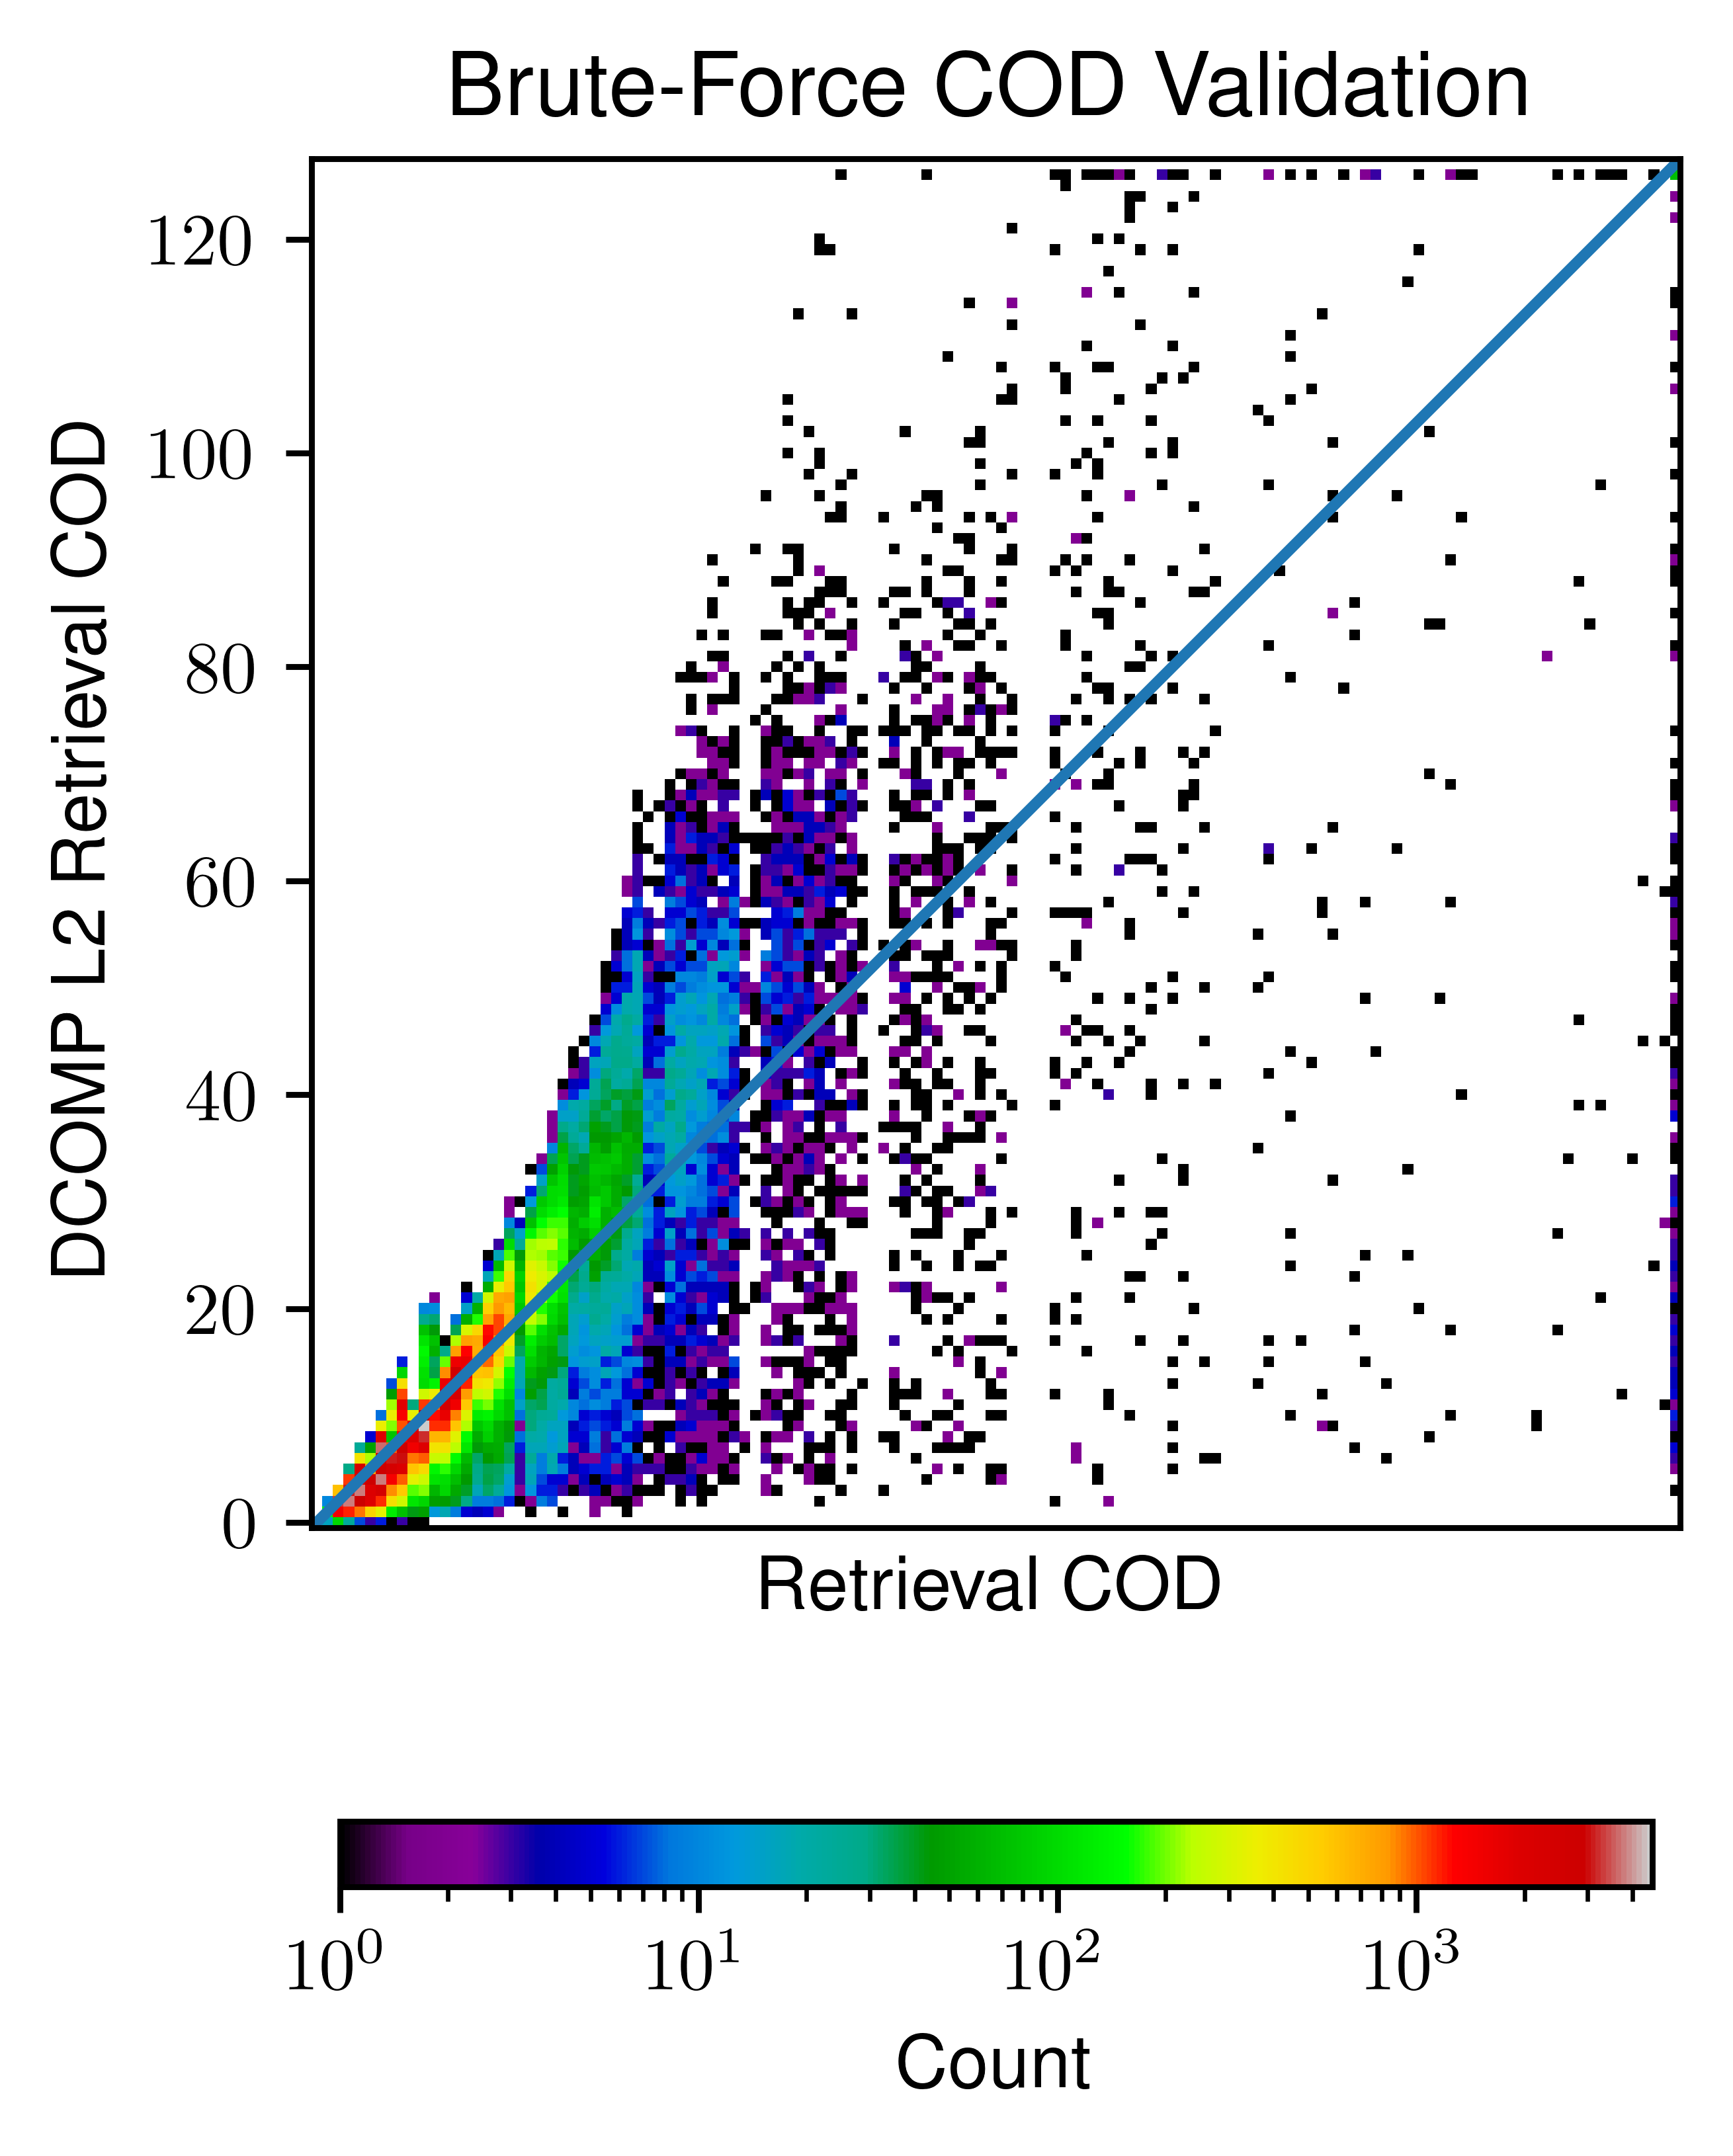
\includegraphics[width=.4\paperwidth]{figs/val_retB_cod.png}
            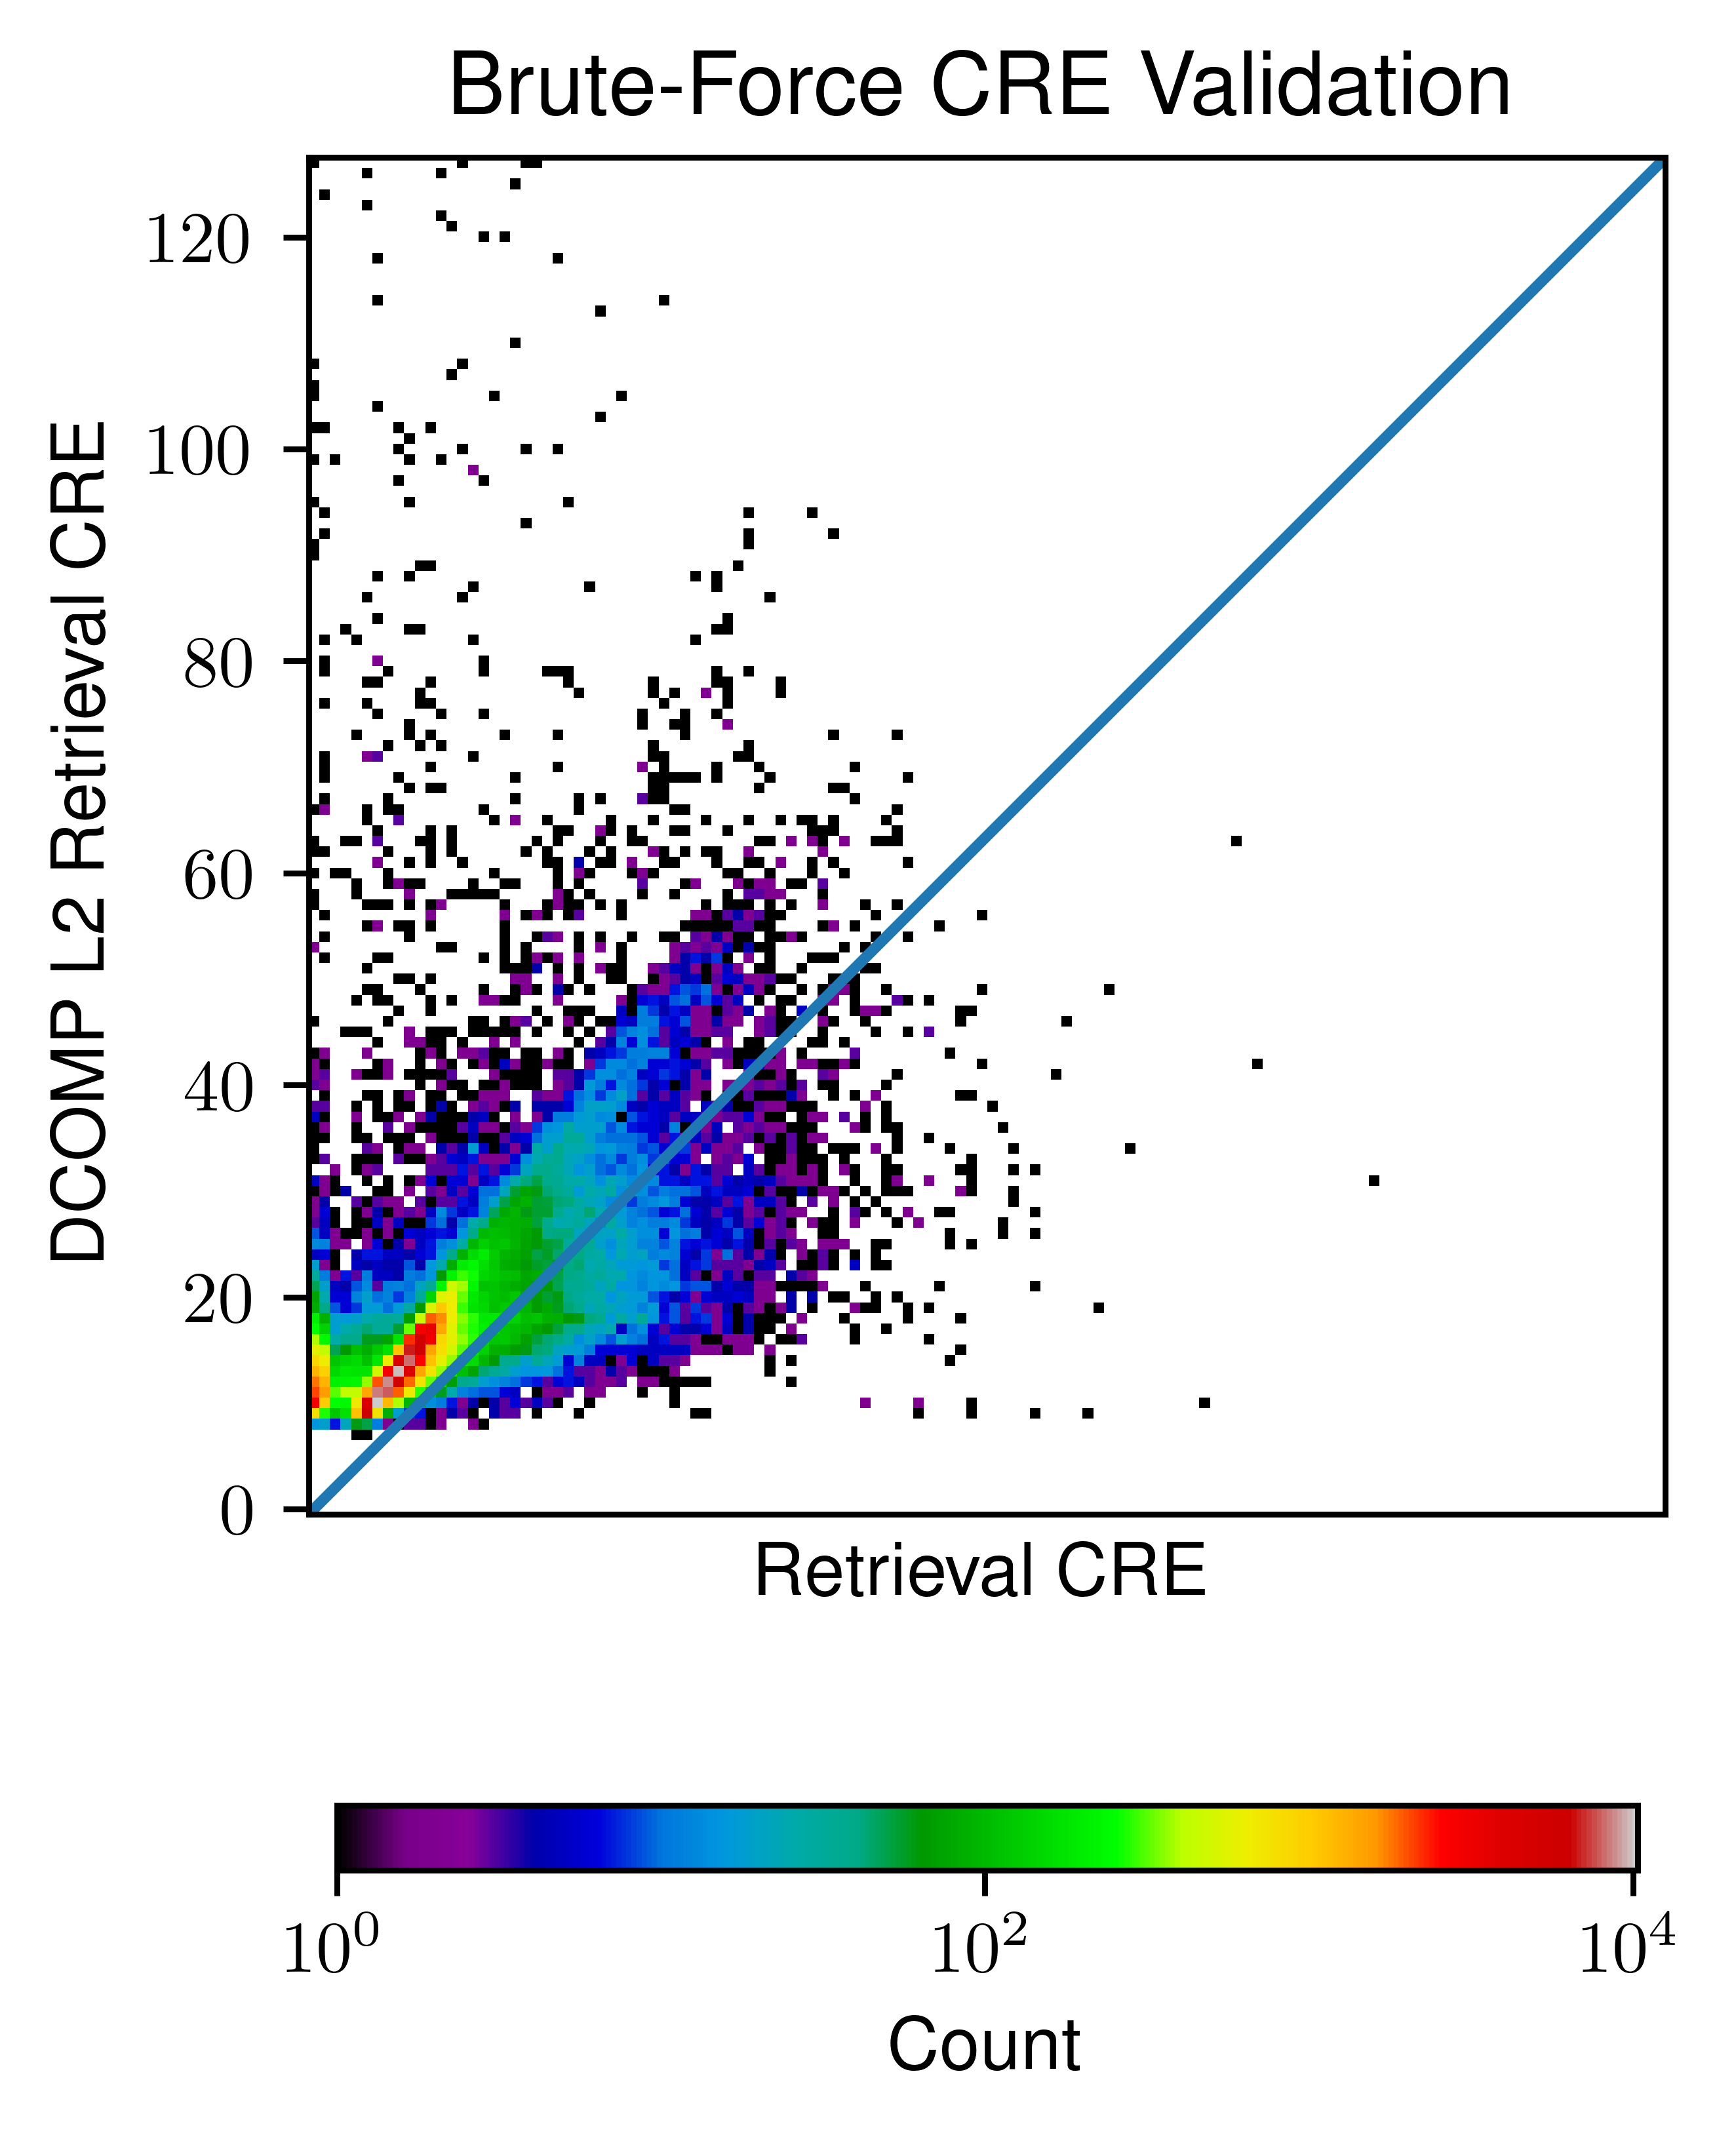
\includegraphics[width=.4\paperwidth]{figs/val_retB_cre.png}
        }
        \makebox[\textwidth]{
            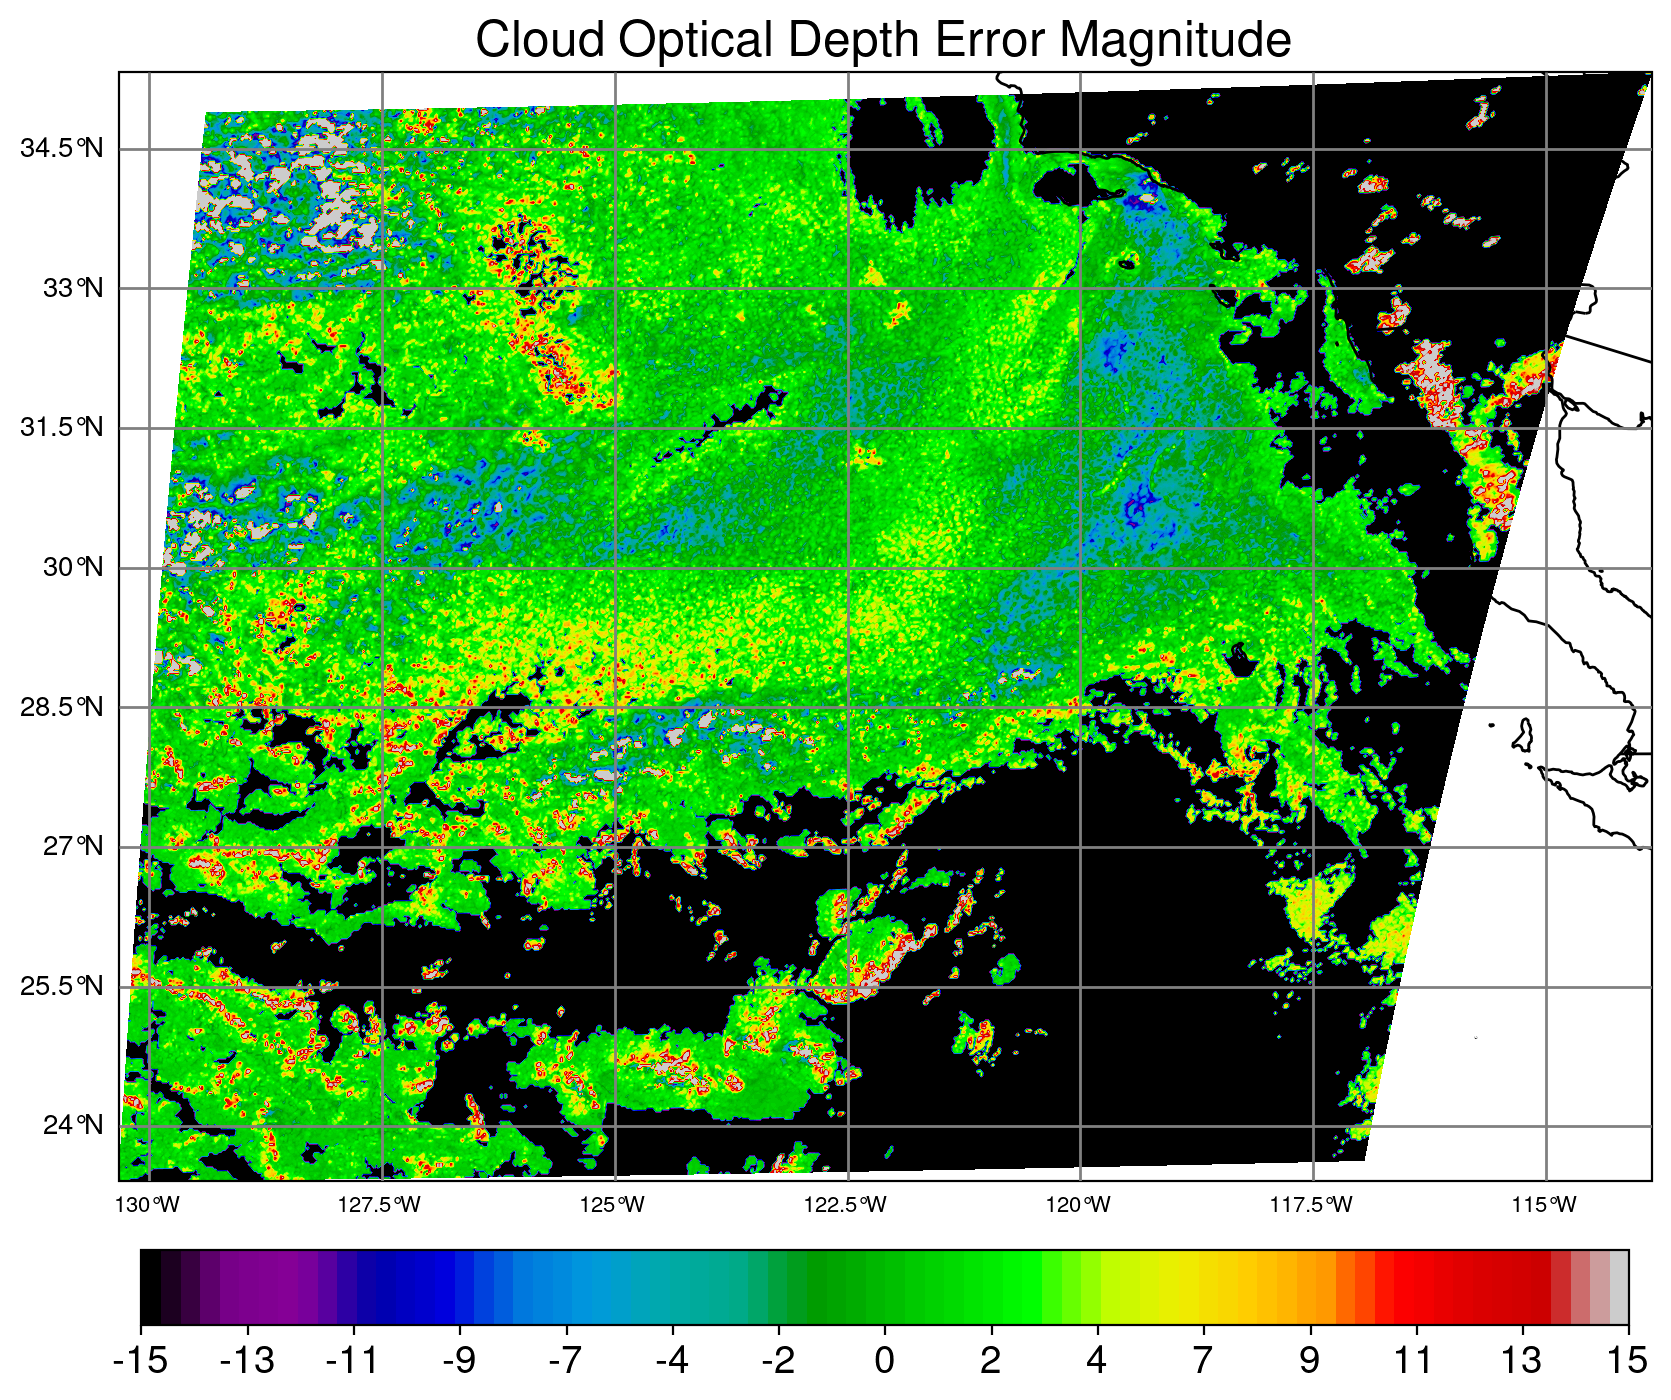
\includegraphics[width=.4\paperwidth]{figs/retB_cod-err.png}
            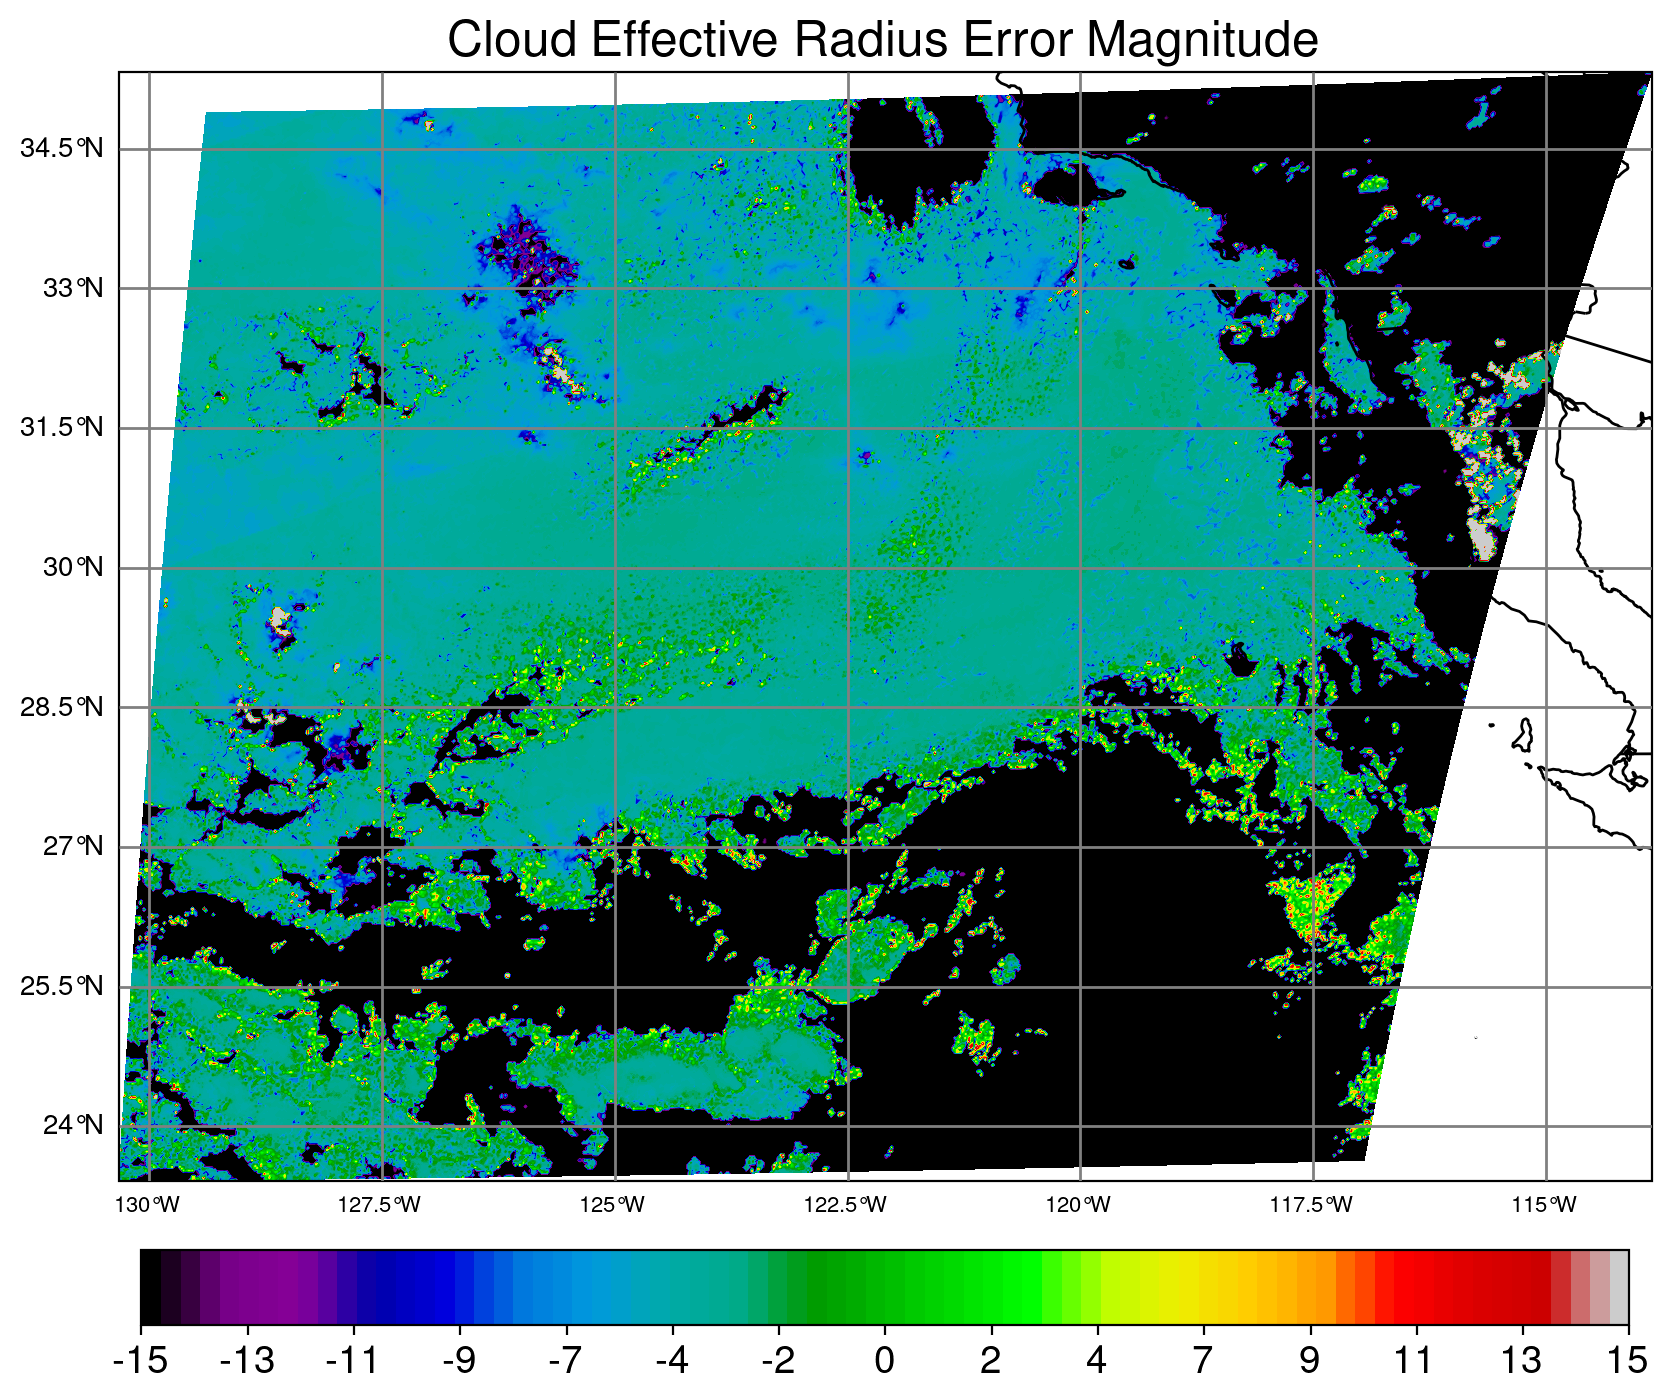
\includegraphics[width=.4\paperwidth]{figs/retB_cre-err.png}
        }
    \end{center}
    \caption{Validation and error characterization of my alternative retrieval method, compared to the official ABI L2 product based on DCOMP. Negative values correspond to an underestimate, and positive values to an overestimate with respect to the L2 product. The validation curve indicates that cloud optical depth product still shows some effects of the discretization of a-priori values, but is clearly more continuous than previous retrievals. Cloud optical depth is generally underestimated where cloud particle size is low, and overestimated where cloud particle size is high. CRE estimates are underestimated overall, especially over very optically-thin clouds regions. See Figure \ref{l2_scal} for L2 reference values.}
    \label{brute}
\end{figure}

\clearpage

\section{Conclusion}

In this project I used ABI L1b radiance data to retrieve the optical thickness and effective radius of liquid oceanic stratiform clouds by following a procedure theoretically outlined by (Nakajima and King, 1990), and practically similar to DCOMP \cite{nakajima_determination_1990}\cite{uw_algorithm_nodate}. This required me to generate lookup tables for top-of-atmosphere radiance using the SBDART radiative transfer numerical model, and to use an optimal estimate inversion technique to determine the best-fitting cloud properties for each observed radiance value. I encountered difficulty when the iterative cost-minimization function scarcely departed from the a-priori values, but developed a separate custom method to perform the inversion, and eventually realized that the setting a-priori error covariance matrix to large values improved the retrievals' performance. Future work for this project may include further investigation of the root causes of initial-value issues, implementation of a forward model capable of handling the emissive $3.9\mu m$ channel, and exploration of alternative cost functions and lookup table architectures.

\section{Appendix}

\vspace{-2em}

\begin{figure}[h!]
    \centering
    \begin{center}
        \makebox[\textwidth]{
            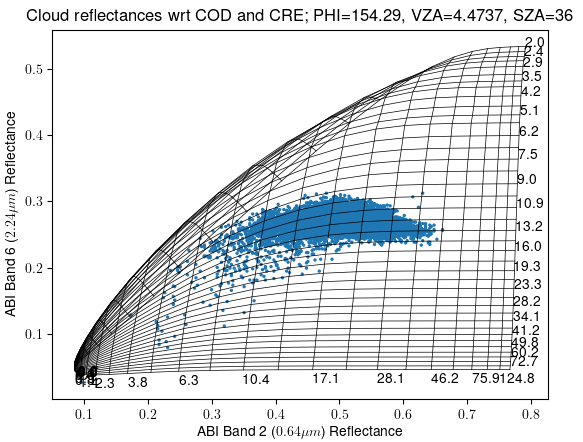
\includegraphics[width=.36\paperwidth]{figs/bispec_deepcloud.png}
            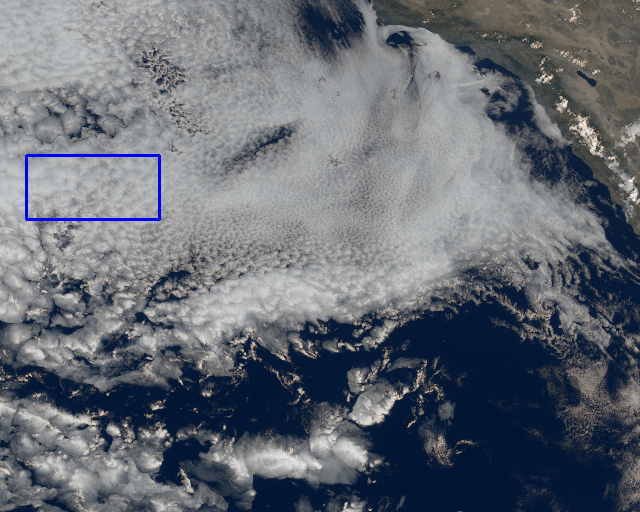
\includegraphics[width=.32\paperwidth]{figs/bispec_deepcloud_domain.png}
        }
        \makebox[\textwidth]{
            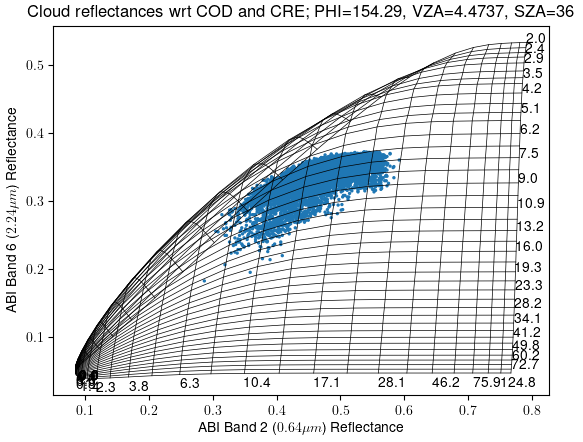
\includegraphics[width=.36\paperwidth]{figs/bispec_seabreeze.png}
            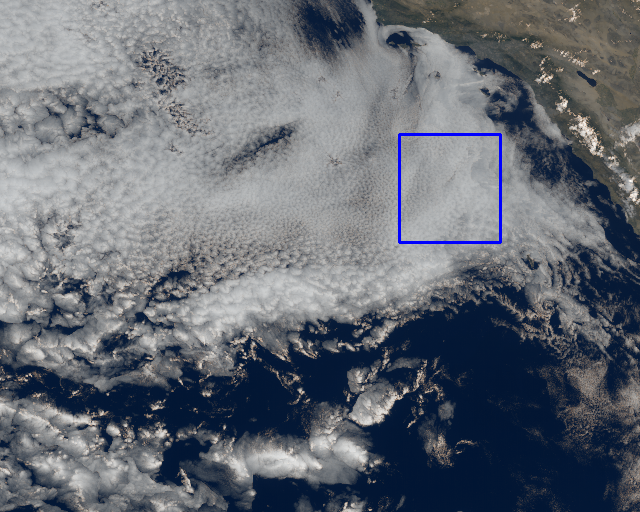
\includegraphics[width=.32\paperwidth]{figs/bispec_seabreeze_domain.png}
        }
    \end{center}
    \caption{Bispectral diagrams generated by sampling region a coarser effective radii and generally optically-thicker region, and a region with finer radii. A demo of the sampling process is available here: \href{https://www.youtube.com/watch?v=fN6za3atMfw}{https://www.youtube.com/watch?v=fN6za3atMfw}.}
    \label{bispec_samples}
\end{figure}

\begin{figure}[h!]
    \centering
    \begin{center}
        \makebox[\textwidth]{
            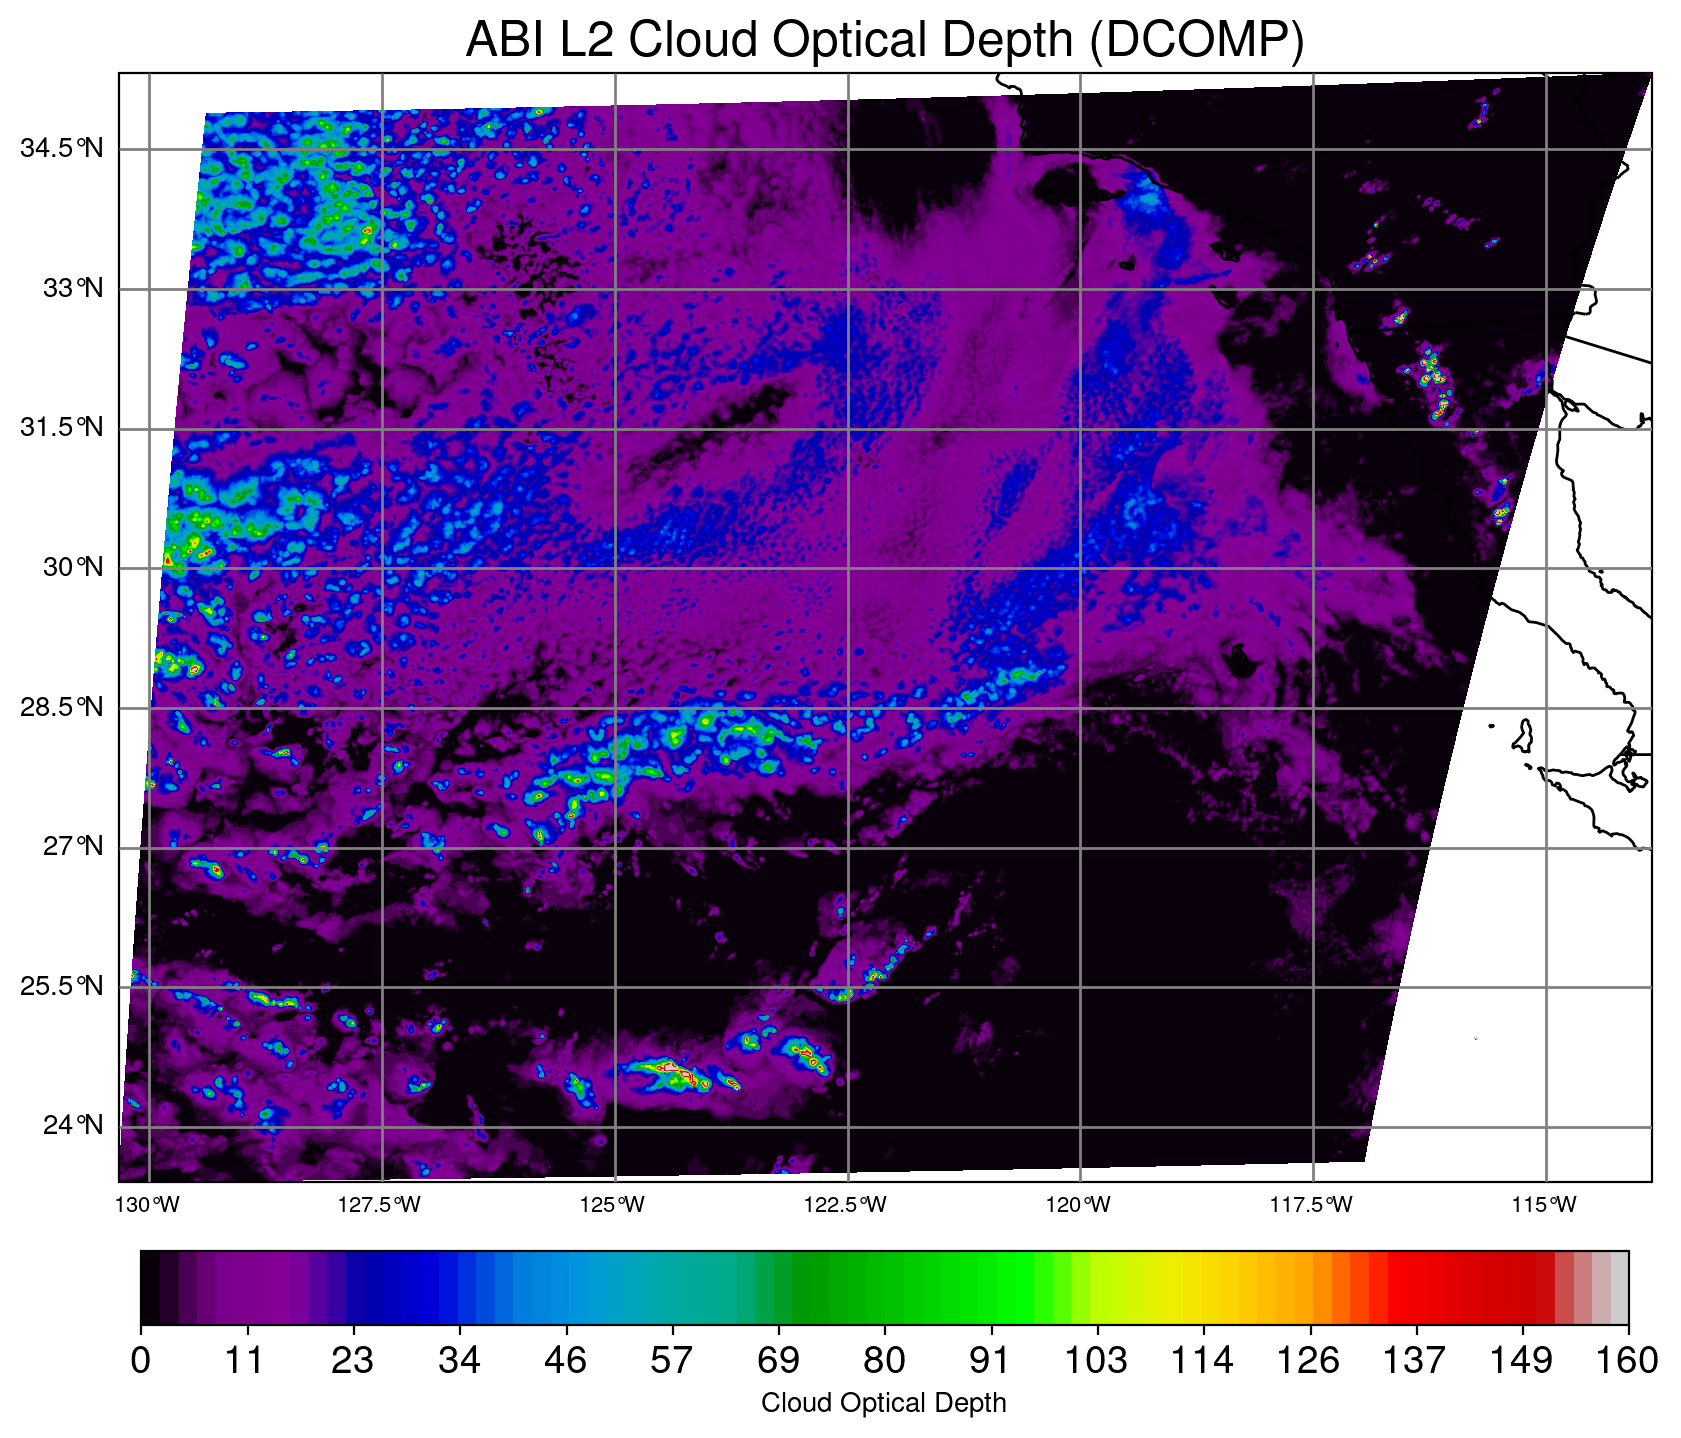
\includegraphics[width=.4\paperwidth]{figs/scal_l2-cod.png}
            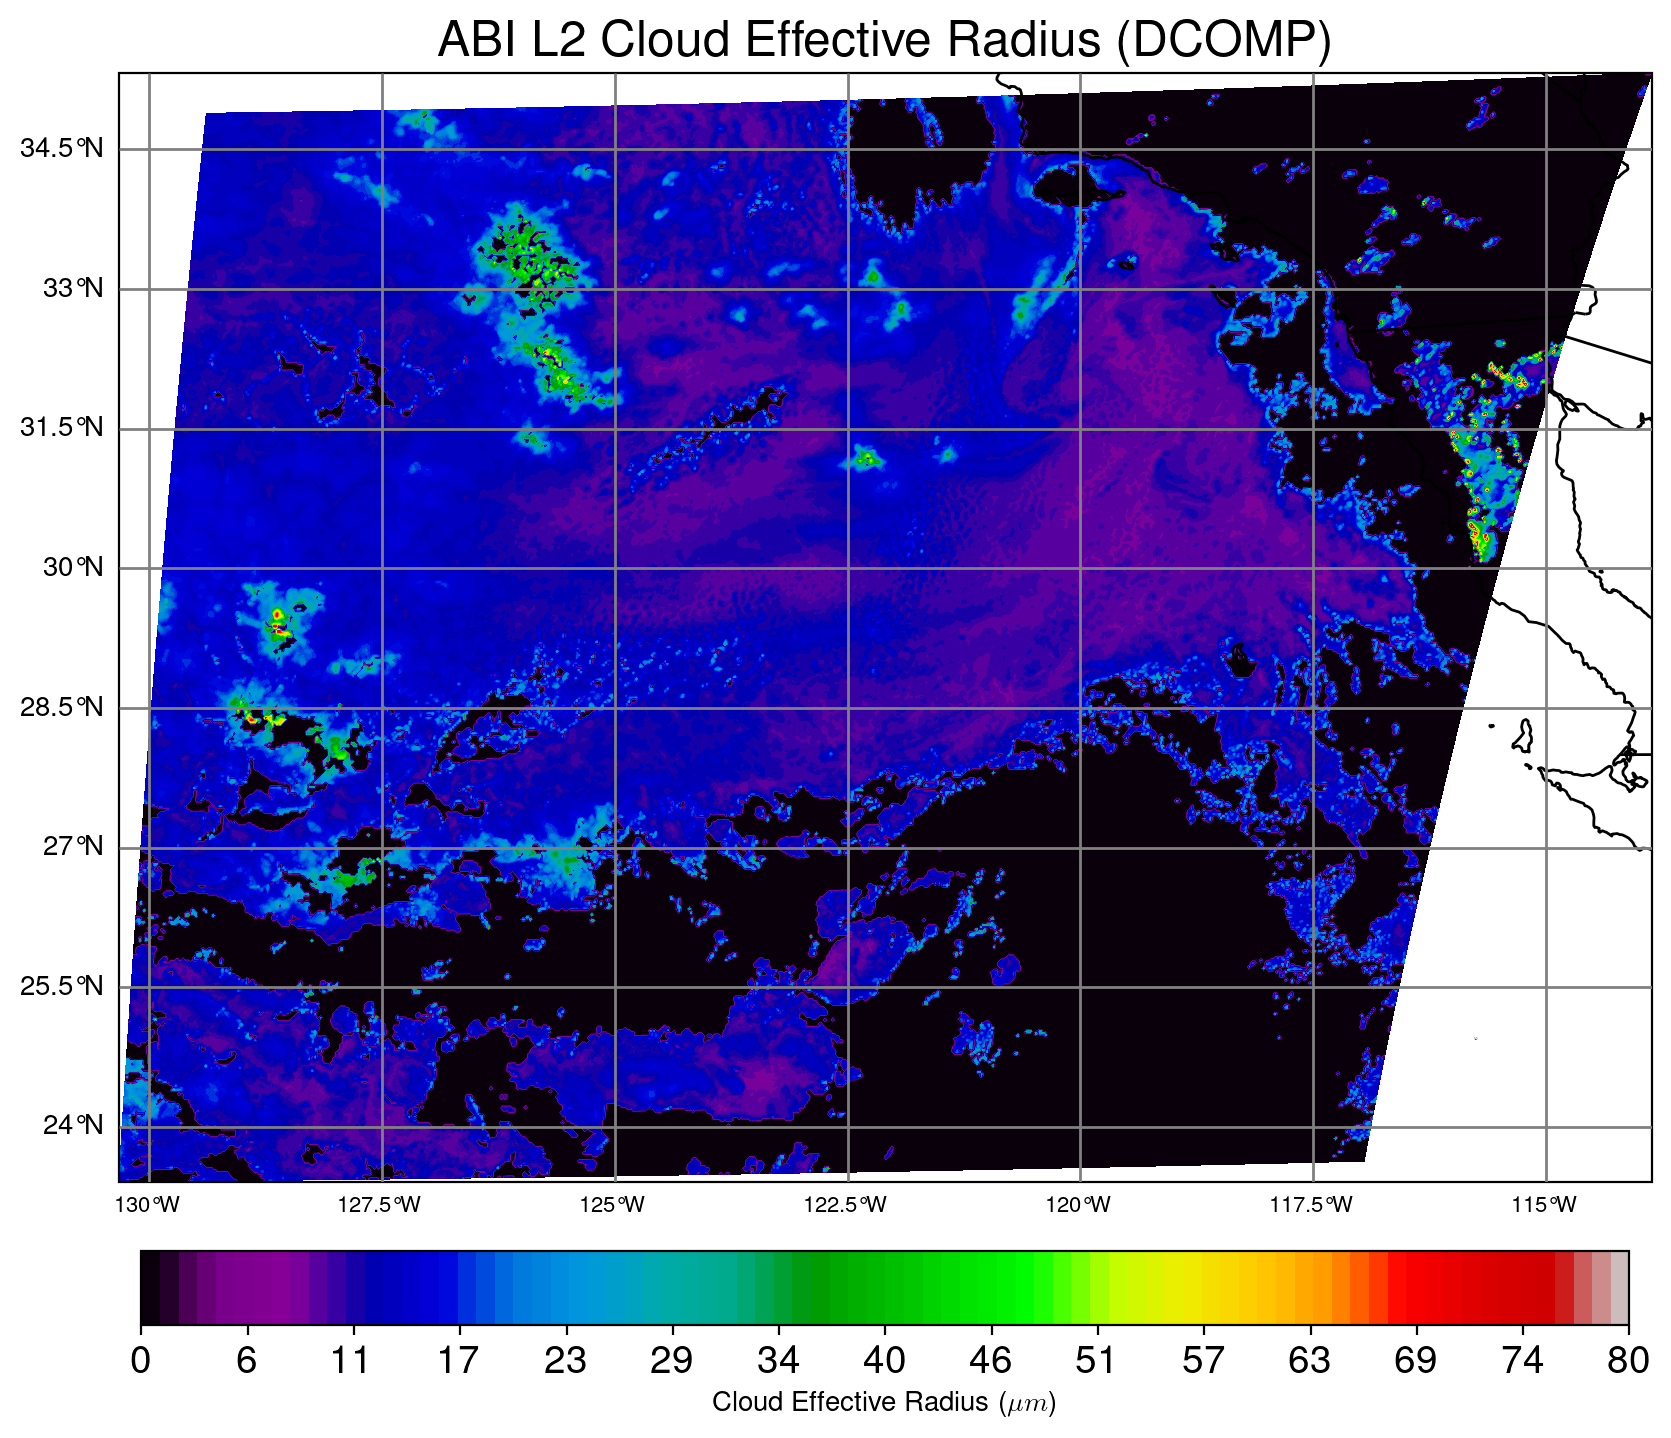
\includegraphics[width=.4\paperwidth]{figs/scal_l2-cre.png}
        }
    \end{center}
    \caption{COD and CRE retrievals from the production DCOMP L2 product.}
    \label{l2_scal}
\end{figure}


\bibliography{main}

\end{document}
